\documentclass[a4paper, openright, twoside]{report}
\usepackage[utf8]{inputenc}
\usepackage[american]{babel}
\usepackage{hyphenat}
\usepackage[activate={true,nocompatibility}, final, tracking=true, kerning=true, factor=1100, stretch=10, shrink=10]{microtype}
% Prevent hyphenization
\tolerance=1
\emergencystretch=\maxdimen
\hyphenpenalty=10000
\hbadness=10000

\usepackage[hmarginratio=1:1,textwidth=360pt,textheight=595.8pt]{geometry}
% Packages
\usepackage{import}

% Math
\newcommand\hmmax{0}
\newcommand\bmmax{0}
\usepackage{bm}
\usepackage{amsmath, amsfonts, amssymb, mathrsfs,extarrows}
\usepackage{commath}
\usepackage[retainorgcmds]{IEEEtrantools}
\usepackage{siunitx}
\usepackage{multirow}
\usepackage[widespace]{fourier}

% Tables
\usepackage{array}
\usepackage{caption}
\usepackage[figuresright]{rotating}
\usepackage{multirow}
\usepackage{makecell}
\usepackage{footnote}
\makesavenoteenv{tabular}

% Algorithm
\usepackage[chapter]{algorithm}
\usepackage{algpseudocode}

%% Citations
\usepackage[numbers]{natbib}
\bibliographystyle{humannat}
\citestyle{egu}
\usepackage[hyphens]{url}
% Bibliography showing in TOC
% \usepackage[nottoc,numbib]{tocbibind}
\usepackage[nottoc]{tocbibind}
\usepackage{scrlayer}
\DeclareNewLayer[
    foreground,
    %textarea,% use only the textarea
    contents={%
      \parbox[b][\layerheight][c]{\layerwidth}
        {\centering Page intentionally left blank.}%
    }
  ]{blankpage.fg}
\DeclarePageStyleByLayers{blank}{blankpage.fg}

% Control structures
\usepackage{ifthen}

% Listing
\usepackage{listings}
\usepackage{xcolor}
\usepackage{float}

% Review notes:
\usepackage{xargs}
\usepackage[textwidth=30mm,textsize=footnotesize]{todonotes} % to create comments (useful to your advisor!)
\newcommandx{\bpf}[2][1=]{\todo[linecolor=blue,backgroundcolor=blue!25,bordercolor=blue,#1]{#2}} % Bernardo notes

% Equation color background
\usepackage{mdframed}

\newmdenv[
    hidealllines=true,
    backgroundcolor=black!20,
    skipbelow=\baselineskip,
    skipabove=\baselineskip
]{highlight}

\newcounter{problem}[chapter]\setcounter{problem}{1}
\renewcommand{\theproblem}{\arabic{chapter}.\arabic{problem}}
\newenvironment{problem}[2][]{%
    \refstepcounter{problem}

    \mdfsetup{hidealllines=true,
    backgroundcolor=black!20,
    skipbelow=\baselineskip,
    skipabove=\baselineskip,
    frametitle={Problem~\theproblem~|~#1}}

\begin{mdframed}[]\relax}{%
\end{mdframed}}

% Enumeration
\usepackage{enumerate}


% Images
\usepackage[labelformat=simple]{subcaption}
\renewcommand\thesubfigure{(\alph{subfigure})}
\renewcommand\thesubtable{(\alph{subtable})}
\usepackage{graphicx}
\graphicspath{ {figures/} }
\usepackage{array}
\usepackage[section]{placeins}
\usepackage{color}
% \usepackage{subcaption}
% \usepackage{subfig}



% Images SVG
\usepackage{import}
\usepackage{xifthen}
\usepackage{pdfpages}
\usepackage{transparent}

\newcommand{\incfig}[1]{
    \def\svgwidth{0.3\columnwidth}
    \import{images/studies/minkowski/fundamental_forms_2D/}{#1.pdf_tex}}


% Floating environment for listings
\floatstyle{plain}
\newfloat{lstfloat}{htbp}{lop}[chapter]
\floatname{lstfloat}{Listing}
\def\lstfloatautorefname{Listing} % needed for hyperref/auroref

% Listing style
\definecolor{codegreen}{rgb}{0,0.6,0}
\definecolor{codegray}{rgb}{0.5,0.5,0.5}
\definecolor{codepurple}{rgb}{0.58,0,0.82}
\definecolor{backcolour}{rgb}{0.95,0.95,0.92}

\lstdefinestyle{mystyle}{
    backgroundcolor=\color{backcolour},
    commentstyle=\color{codegreen},
    keywordstyle=\color{blue},
    numberstyle=\tiny\color{codegray},
    stringstyle=\color{codepurple},
    basicstyle=\fontsize{7}{10}\selectfont,
    breakatwhitespace=false,
    breaklines=false,
    captionpos=b,
    keepspaces=true,
    numbers=left,
    numbersep=5pt,
    showspaces=false,
    showstringspaces=false,
    showtabs=false,
    tabsize=2
}

\lstset{style=mystyle}

\makeatletter
\newcommand*{\shifttext}[2]{%
  \settowidth{\@tempdima}{#2}%
  \makebox[\@tempdima]{\hspace*{#1}#2}%
}
\makeatother

\usepackage{pythonhighlight}

% Appendices
\usepackage[toc,page]{appendix}

% Headers and footers



\usepackage{fancyhdr}
% \renewcommand{\chaptermark}[1]{\markboth{\thechapter.\ #1}{}}
% \renewcommand{\sectionmark}[1]{\markright{\thesection.\ #1}}

% \fancypagestyle{plain}{
% \fancyhf{}
% \fancyhead{}% remove default header entries
% \fancyhead[RE]{a\textsc{\leftmark}}
% \fancyhead[LE]{\thepage}
% \fancyhead[LO]{\textsc{\rightmark}}
% \fancyhead[RO]{\thepage}
% \renewcommand{\headrulewidth}{0.1pt} }
% \pagestyle{plain}

\fancypagestyle{firststyle}
{
   \fancyhf{}
    \fancyhead{}% remove default header entries
   \fancyfoot[C]{Porto, September 2021}
   \renewcommand{\headrulewidth}{0pt}
\renewcommand{\footrulewidth}{0.1pt}
    \fancyfootoffset{-0.25\textwidth}
}

\pagestyle{fancy}
\fancyhf{}
\renewcommand{\chaptermark}[1]{\markboth{\thechapter.\ #1}{}}
\renewcommand{\sectionmark}[1]{\markright{\thesection.\ #1}}
\fancyhead{}% remove default header entries
\fancyhead[RE]{\nouppercase\leftmark}
\fancyhead[LE]{\thepage}
\fancyhead[LO]{\nouppercase\rightmark}
\fancyhead[RO]{\thepage}
\renewcommand{\headrulewidth}{0.1pt}

\newenvironment{dedication}
  {%\clearpage           % we want a new page          %% I commented this
   \thispagestyle{empty}% no header and footer
   \vspace*{\stretch{1}}% some space at the top
   \itshape             % the text is in italics
   \raggedleft          % flush to the right margin
  }
  {\par % end the paragraph
   \vspace{\stretch{3}} % space at bottom is three times that at the top
   \clearpage           % finish off the page
  }


%Custom FramedBox Environment
%%Loading 'float' package
\usepackage{float}
%%Customize 'boxed' float style (caption above the body)
\makeatletter
\newcommand\fs@boxedtop
 {\fs@boxed
  \def\@fs@mid{\vspace\abovecaptionskip\relax}%
  \let\@fs@iftopcapt\iftrue
 }
\makeatother
%%Defining float commands
\floatstyle{boxedtop}
\floatname{framedbox}{Box}
\newfloat{framedbox}{hbt}{lob}[chapter]

% Symbols
%% Differential Upright "d"
\newcommand{\ud}{\,\mathrm{d}}
%% Assemble operator
\DeclareMathOperator*{\assemble}{\text{\Large $ \mathsf{A} $}}
%% Matrices and vectors
\newcommand{\vect}[1]{\bm{#1}}
\newcommand{\mat}[1]{\bm{#1}}
\newcommand{\boldsf}[1]{\boldsymbol{\mathsf{#1}}}

\DeclareMathAlphabet{\pazocal}{OMS}{zplm}{m}{n}

\title{Numerical Methods}
\author{José Luís Passos Vila-Chã}
\date{May 2021}


\pagenumbering{roman}

%Hypertext marks
\usepackage[pdftitle={NLMFEA_assignment},
			pdfauthor={JoseVila-Cha},
			pdfdisplaydoctitle=true,
			colorlinks=true,
			% Eletronic Version
             linkcolor=orange,
             citecolor=teal,
            % Print Version
            % linkcolor=black,
            % citecolor=black,
            bookmarks=true,
            bookmarksopen=false,
            bookmarksnumbered=true]{hyperref}

\usepackage[intoc]{nomencl}
\usepackage{xstring}
\usepackage{xpatch}
\patchcmd{\thenomenclature}
  {\leftmargin\labelwidth}
  {\leftmargin\labelwidth\itemindent 1em }
  {}{}

% Nomenclature

\makenomenclature
\renewcommand{\nomname}{Notation}
%% This code creates the groups
% -----------------------------------------
\usepackage{etoolbox}
\newcommand{\nomenclheader}[1]{%
  \item[\hspace*{-\itemindent}\bfseries\LARGE#1\vphantom{$\Bigg \vert $}]}
\renewcommand\nomgroup[1]{%
  \IfStrEqCase{#1}{%
   {A}{\nomenclheader{General abbreviations}}%      A - Acronyms
   {N}{\nomenclheader{General notation}}% R - Roman
   {O}{\nomenclheader{Operators and symbols}}% G - Greek
   {D}{\nomenclheader{Sets, domains and boundaries}}% G - Greek
   {S}{\nomenclheader{Subscripts and superscripts}}%  S - Superscripts
   {C}{\nomenclheader{Accents}}%    U - Subscripts
   {V}{\nomenclheader{Variables}}% X - Other Symbols
  }%
  \vspace{20pt}
}
\setlength{\nomitemsep}{-1pt}
% -----------------------------------------



\begin{document}
\begin{titlepage}
\thispagestyle{firststyle}
\begin{center}
   \begin{minipage}[c][10cm][l]{0.9\textwidth}

        
\includegraphics[width=0.6\textwidth]{figures/university}

        \vspace{3.5cm}
        \huge
       \textbf{FFT-based Homogenization Methods}

       \vspace{1.5cm}
        \small
       \textit{Professor:}\\
       \normalsize
       Francisco Manuel Andrade Pires 	\\

       \vspace{0.5cm}


         \small
        \textit{Student:}\\
        \vspace{0.5cm}
       \normalsize
       \!José Luís Passos Vila-Chã
       \vspace{8cm}


        \centering
       \small
       Report presented under the scope of the\\ Doctoral Program in Mechanical Engineering

   \end{minipage}
   \end{center}
\end{titlepage}

\newpage\null\thispagestyle{blank}\newpage

\setcounter{tocdepth}{2}
\tableofcontents


\listoffigures

\newpage\null\thispagestyle{blank}\newpage

\listoftables

\newpage\null\thispagestyle{blank}\newpage

\pagenumbering{gobble}
\pagenumbering{arabic}
\pagestyle{fancy}
\chapter{Introduction}

\chapter{FFT-based methods for mechanical problems} \label{chapter:fft_based_homogenization}

In the following, an overview of the literature on FFT-based methods for the determination of the overall and local response of a composite material from actual images or morphological simulations of its microstructure is presented.

To establish some context, let the microstructure of the material be represented by a periodic cell \(\Omega_\mu\).
The material response at a point \(\bm Y \in \Omega_\mu\) is specified by the constitutive relation \(\bm{\sigma}_\mu(\bm{Y}\), \(\bm\varepsilon_\mu(\bm{Y}))\) assigning the stress response \(\bm\sigma_\mu\) to a given strain \(\bm\varepsilon_\mu\) locally at \(\bm Y\).
Furthermore, the total strain \(\bm\varepsilon_\mu\) is split into a homogeneous average strain tensor present at the macroscopic point \(\bm X\), \(\bm \varepsilon(\bm X)\), and an \(\Omega_\mu\)-periodic fluctuating strain field \(\tilde{\bm \varepsilon}_\mu(\bm Y)\), i.e.
\begin{equation}
\bm\varepsilon_\mu(\bm{Y})=\bm \varepsilon(\bm X)+\tilde{\bm \varepsilon}_\mu(\bm{Y}) \text { for } \bm Y \in \Omega_{\mu,0}, \quad \int_{\Omega_{\mu,0} } \tilde{\bm\varepsilon}_\mu(\bm{Y}) \mathrm{d} v=\bm{0}.
\end{equation}
The average strain \(\bm \varepsilon(\bm X)\) represents a given macro-scale excitation, while the fluctuating micro-scale strain field \(\tilde{\bm\varepsilon}_\mu\) is the primary unknown.

The fluctuating strain field \(\tilde{\bm\varepsilon}_\mu\) is determined by the stress equilibrium and strain compatibility conditions, which under quasi-static assumptions and in small strains read as,
\begin{gather}\label{eq:diff_equilibrium_equation}
\operatorname{div}\left[\bm{\sigma}_\mu\left(\bm Y, \bm \varepsilon(\bm X)+\tilde{\bm\varepsilon}_\mu(\bm Y)\right)\right]=0 \text { for } \bm Y \in \Omega_{\mu,0},\\
\label{eq:compatibility_equations}
\tilde{\bm\varepsilon}_\mu \in \pazocal{E}=\left\{\bm{\nabla}_0^{\mathrm{s}} \tilde{\bm{u}}_\mu\ |\ \text{\(\tilde{\bm{u}}_\mu\) is an \(\Omega_\mu\)-periodic displacement field}\right\},
\end{gather}
where \(\bm{\nabla}_0^{\mathrm{s}}\)\nomenclature[V]{\bm{\nabla}_0^{\mathrm{s}}}{Symmetrized gradient operator} stands for the symmetrized gradient operator.
For the numerical treatment, the local problem \eqref{eq:diff_equilibrium_equation} is recast into the weak form, which amounts to finding \(\tilde{\bm\varepsilon}_\mu \in \pazocal{E}\) such that
\begin{equation} \label{eq:weak_form_equilibrium_eq}
\int_{\Omega_{\mu,0}} \delta \tilde{\bm\varepsilon}_\mu(\bm{Y}): \bm{\sigma}_\mu\left(\bm Y, \bm \varepsilon(\bm X)+\tilde{\bm\varepsilon}_\mu(\bm Y)\right) \mathrm{d}v = 0,
\end{equation}
holds for all \(\delta \tilde{\bm\varepsilon}_\mu \in \pazocal{E}\) (where use has been made of the periodicity of the problem eliminate the boundary term).

The FFT based methods, first introduced by \cite{moulinec_fast_1994, moulinec_fft-based_1995}, enjoy wide usage across many domains.
They have been integrated into efficient and robust two-scale FE-FFT-based computatinal approaches \citep{kochmann_efficient_2018-1} and now even figure in comercial software such as DAMASK \citep{roters_damaskdusseldorf_2019} and FeelMath \citep{schwichow_geodict_2020, fraunhofer_itwm_feelmath_2020}.
Their application ranges from crystal plasticity (e.g. \cite{lebensohn_n-site_2001, shanthraj_numerically_2015, kochmann_efficient_2018, lebensohn_spectral_2020, wicht_efficient_2020}), hypoelasticity (e.g. \cite{ma_fft-based_2019}), failure and damage (e.g. \cite{ernesti_fast_2020, ernesti_fft-based_2021, geus_damage_2016, magri_fft_2021, wang_progressive_2018}) and multi-physics simulations (e.g. \cite{vinogradov_accelerated_2008,brenner_computational_2010,shanthraj_spectral_2019, gokuzum_multiscale_2019, zhou_accelerated_2020,wicht_computing_2020}).
They have also been used in the contex of reduced order models (e.g. \cite{kochmann_simple_2019, gierden_geometrically_2021}).

Comparisons between the FEM and the FFT-based methods can be found in \cite{michel_effective_1999} and \cite{vondrejc_energy-based_2020}.
The first focuses on the "basic scheme" and concludes that the FFT-based method is much faster than FEM when the contrast between phase properties is not too large.
This advantage decreases as the contrast increases, in favor of the FEM.
In the second contribution, Galerkin-based formulations are considered.
The advantage of FEM for the case of rough data with jumps in material coefficients regarding both memory usage and speed is reasserted.
The results for continuous material coefficients are inconclusive.


The main classification scheme adopted follows \cite{zeman_finite_2017} and is based on the discretization approach.
The first set of methods, which include the original contribution from \cite{moulinec_fast_1994}, are labeled as "Conventional FFT" and the second class as "Variational FFT".
In the last section, a few methods not fitting this classification scheme are also presented.


\section{Conventional FFT}

% Lippmann-Schwinger
Following \cite{zeman_finite_2017}, the "Conventional FFT" methods, based on the basic scheme by \cite{moulinec_fast_1994}, are derived from the following integral equation for the fluctuating strains \(\tilde{\bm\varepsilon}_\mu \in \pazocal{E}\),
\begin{equation} \label{eq:int_lippmann_schwinger}
\int_{\Omega_\mu} \bm \Gamma^{\mathrm{ref}}(\bm{Y}-\bm{Y}'): \bm{\sigma}_\mu\left(\bm{Y}', \bm{\varepsilon}(\bm X)+\tilde{\bm \varepsilon}_\mu(\bm{Y}')\right) \mathrm{d} v'=\mathbf{0}\quad \text { for all } \bm{Y} \in \Omega_\mu,
\end{equation}
where \(\bm \Gamma^{\text {ref }}\) is the Green function of the reference problem.
This reference problem is an auxiliary local problem with the homogeneous constitutive relation
\begin{equation}
\bm \sigma_\mu(\bm{Y}, \bm \varepsilon(\bm{Y}))=\boldsf D^{\mathrm{ref}}: \bm\varepsilon(\bm{Y}) \text { for } \bm{Y} \in \Omega_\mu,
\end{equation}
where \(\boldsf D^\mathrm{ref}\) is the elasticity tensor of the reference material.
% normal
In the seminal contribution by \cite{moulinec_fast_1994, moulinec_fft-based_1995}, Equation~\eqref{eq:int_lippmann_schwinger} is solved using a fixed-point iteration scheme after discretizing it through a point collocation method, the basis function being trigonometric polynomials \citep{zeman_finite_2017}.
It is originally formulated for linear elasticity and small strains.
In \cite{michel_computational_2000, michel_computational_2001}, the authors extend this scheme to materials with non-linear mechanical behavior laws.

It has become very popular as a method used for the determination of local fields and effective properties since it does not require meshing.
Thus, it allows the direct use of experimental images obtained by advanced imaging techniques such as micro-computed tomography.
Besides, from a computational standpoint, it is also a very fast and memory-efficient method.
It enjoys from current implementations of the Fast Fourier transform, which are extremely powerful.
Moreover, the scheme supports matrix-free solvers, even for strongly non-linear materials.
Lastly, the method is also simple to code and use.

Despite all these favorable characteristics, the method also has some drawbacks.
It is not suitable for composites with infinite contrast between the phases and near interfaces between phases where large differences in the material properties are found, spurious features have also been reported \citep{ma_numerical_2021}.
Furthermore, the convergence rate as a function of the material contrast is only linear.

% paragraph mesh
As already mentioned, this class of methods uses a regular mesh, where the basis functions are trigonometric polynomials.
Exceptions are \cite{bonnet_effective_2007}, \cite{monchiet_polarization-based_2012}, \cite{monchiet_combining_2015} and \cite{nguyen_derivation_2021}.
In the first three, the exact Fourier transforms of the elasticity tensor are used.
This can be achieved because the Fourier transforms of the characteristic functions of the inclusion phases are known, being limited to circles and ellipses.
The last work uses the approximate Fourier transform of the elasticity tensor, but the phases are not limited to circles and ellipses.
More complex phase domains are approximated through the union of polygons and polyhedra (e.g. flower-shaped inclusions in 2D and torus-shaped inclusion in 3D) for which the Fourier transforms of the characteristic functions are known.


A further sub-classification for the "Conventional FFT" methods can be introduced, according to \cite{schneider_barzilai-borwein_2019}.
For the first kind, each iterate satisfies the mechanical compatibility condition, whereas, for the second kind, compatibility is only ensured upon convergence.
The polarization schemes and solvers based on the Hashin-Shtrikman principle constitute the former kind.
The latter includes the conjugate gradient method, the Newton-scheme (coupled to different linear solvers), and the fast gradient methods.

% polarization
Regarding the contributions based on polarization, the original work is due to \cite{eyre_fast_1999}.
It is developed in the context of electrical conductivity, hence the use of the term "polarization" in connection with these schemes.
Accordingly, the procedure iterates on the polarization field, and not on the strain field, as per usual.
Combined with the rewriting of the expression for the original scheme, this leads to faster convergence rates, superlinear, when compared with the "basic scheme", as a function of the material contrast.
In \cite{michel_computational_2001} this approach is extended to linear elasticity, and a related approach based on an augmented Lagrangian is also introduced.
Convergence for infinite contrast is achieved for this last method.
Lastly, in \cite{monchiet_polarization-based_2012} a further extension is proposed, with the scheme suggested including both of the polarization-based works previously mentioned.
Convergence for infinite contrast is likewise achieved.
In \cite{schneider_polarization-based_2019} two flaws in these methods are pointed out in the non-linear context.
Firstly, the optimal choice of algorithmic parameters is only known for the linear elastic case.
Secondly, in its original version, each iteration of the polarization scheme requires solving a nonlinear system of equations for each voxel.
The authors cast these methods into a simpler form using the Douglas-Rachford splitting, thus, avoiding the solution of non-linear equations in each iteration.
In \cite{moulinec_comparison_2014}, \cite{moulinec_comparison_2014-1} and \cite{schneider_polarization-based_2019} comparisons between these methods and others can be found.
Finally, the linear solvers of \cite{brisard_fft-based_2010, brisard_combining_2012} also belong to the class of polarization schemes, although they operate on a different polarization \citep{schneider_lippmannschwinger_2020}.

Beyond the "basic scheme" of \cite{moulinec_fast_1994} further improvements within the same framework have been proposed.
% linear small strain
In the first place improvements still dealing with linear behavior at small strains are introduced.
In the original approach, a fixed point iteration/Richardson iteration/Neumann series-based scheme is used (see \cite{moulinec_convergence_2018} for an in-depth convergence analysis).
It is the most memory-efficient method available in its class and it is also robust but slow for highly contrasted problems.
Moreover, the only role of the (material-dependent) reference problem is to ensure the convergence of the Richardson iteration scheme used to solve the resulting system of linear equations.
As an alternative, \cite{zeman_accelerating_2010} propose a conjugate gradient-based approach.
It proceeds from the discretization of the governing integral equation by the trigonometric collocation method to give a linear system that can be efficiently solved by conjugate gradient methods.
The authors claim a significant increase of the convergence rate for problems with high-contrast coefficients at a low overhead per iteration.
The scheme is also independent of the reference problem.

%non-linear
According to \cite{kabel_efficient_2014}, regarding non-linear problems, be it concerning small or large strain, there are two solution strategies.
Firstly, a fixed point iteration can be employed to solve the nonlinear equation introduced in \cite{moulinec_numerical_1998} for small deformations and extended to large deformations in \cite{eisenlohr_spectral_2013}.
Also for small deformations, \cite{schneider_fft-based_2017} and \cite{schneider_dynamical_2020} present the use of the fast gradient methods (Nesterov's method, heavy-ball method, and Fletcher-Reeves CG), which also forego the linearization of the nonlinear equations.
The fast gradient methods combine fast convergence with a low memory footprint.
However, they suffer from a delicate parameter selection \citep{schneider_dynamical_2020}.

Alternatively, one can use the Newton or quasi-Newton methods to tackle the nonlinear problem by solving a sequence of linear problems.
% small strain
% newton
% conjugate gradient
In the context of small strains, \cite{gelebart_non-linear_2013} solve the linearized equations found through the Newton method using the conjugate gradient scheme.
Low sensitivity to the reference material and improved efficiency, for a soft or a stiff inclusion, when compared to the "basic scheme" is reported.
In addition to prescribed macroscopic strain, the proposed method is extended to mixed loadings.

% large strain
% newton
% fixed-point
Concerning large strains, using Newton methods to linearize the nonlinear equations, \cite{lahellec_analysis_2003} present a scheme where a fixed-point approach is used to solve the linearized equations.
% newton-krylov
In \cite{kabel_efficient_2014}, fixed-point schemes are also considered, in addition to Newton-Raphson and Netwon-Krylov/conjugate gradient methods.
In connection to the last method, a memory-efficient version is also presented.

% quasi-newton
Quasi-Newton methods are available in the literature, as well.
% lbfgs
In \cite{wicht_quasinewton_2019} two algorithms based on the Broyden-Fletcher-Goldfarb-Shanno (BFGS) method, one of the most powerful Quasi-Newton schemes, are introduced.
More specifically, the BFGS update formula is utilized to approximate the global Hessian or the local material tangent stiffness.
Both for Newton and Quasi-Newton methods, a globalization technique is necessary to ensure global convergence.
Specific to the FFT-based context, a Dong-type line search is promoted, avoiding function evaluations altogether.
% Anderson acceleration
Another Quasi-Newton method, mentioned in \cite{wicht_quasinewton_2019} and extended to polarization methods in \cite{wicht_anderson-accelerated_2021}, is the Anderson acceleration method.
It is a method for improving the convergence behavior of fixed-point iterations, where derivatives of the fixed-point mapping are not available.
Based on a limited number (the so-called depth) of previous iterates, Anderson acceleration generates the next iterate based on a mixture of previous iterates, where the mixing coefficients
solve an associated low-dimensional optimization problem.
% Barzilai-Borwein
In \cite{schneider_barzilai-borwein_2019} the Barzilai-Borwein is applied to the problem at hand.
It may be interpreted as the basic scheme with adaptive time-stepping (or, equivalently, adaptive reference material).
Thus, it has a low memory footprint but is competitive in terms of convergence speed when compared to the solvers mentioned above.
However, it is an intrinsically non-monotone method, ie, the residual is not monotonically decreasing from one iteration to the next.
This behavior is unfamiliar and may limit its applicability for industrial applications.

Table~\ref{tab:methods} reproduces a Table found in \cite{wicht_quasinewton_2019} detailing the memory footprint and other characteristics regarding the different solvers available.


\begin{table}
\caption{Summary of the performance comparison between the investigated solution schemes \citep{wicht_quasinewton_2019}}
\label{tab:methods}
 \begin{tabular}{l l l}
 \hline
 Solution scheme & \makecell{Memory footprint\\ (strain-like fields)} & Summary and remarks\\
 \hline\hline
 Basic scheme & 1 & \makecell[l]{\textbullet\ Gradient descent method\\ \textbullet\ Lowest memory requirements \\ \textbullet\ Slowest among the studied solvers}\\
 \hline
 Anderson acceleration & \(2m+2\) & \makecell[l]{\textbullet\ Limited-memory Quasi-Newton\\ method\\ \textbullet\ Optimal depth \(m\) between 2 and 5 \\ \textbullet\ Accelerates the basic scheme but\\ slower than the remaining\\ algorithms}\\
 \hline
 L-BFGS & \(2m+4\) & \makecell[l]{\textbullet\ Limited-memory Quasi-Newton\\ method\\ \textbullet\ Optimal depth \(m\) between 2 and 5 \\ \textbullet\ Outperformed by the more memory-\\-efficient Barzilai-Borwein method}\\
 \hline
 Barzilai-Borwein & \(2\) & \makecell[l]{\textbullet\ Gradient descent with step size\\ based on Quasi-Newton methods\\ \textbullet\ Nonmonotonic convergence\\ behavior \\ \textbullet\ Fastest choice for inexpensive\\ material laws}\\
 \hline
 Newton-CG & \(8.5\) & \makecell[l]{\textbullet\ Inexact Newton method\\ \textbullet\ Highest efficiency in combination\\ with Eisenstat and Walker's\\ forcing-term choice 2\\ \textbullet\ Requires computing the\\ material tangent\\ \textbullet\ Fastest choice for expensive\\ material laws}\\
 \hline
 BFGS-CG & \(10.5\) & \makecell[l]{\textbullet\ Inexact Quasi-Newton method\\ \textbullet\ Uses the BFGS update to approximate\\ the material tangent\\ \textbullet\ Matches performance of\\ Newton-CG for small load steps,\\ slightly slower otherwise}\\
 \hline\hline
\end{tabular}
\footnotesize{\(\vphantom{\Big \vert}\)Abbreviations: BFGS, Broyden-Fletcher-Goldfarb-Shanno; CG, conjugate gradient.}
\end{table}

\section{Variational FFT}

According to \cite{zeman_finite_2017} the so-called "Variational FFT" schemes, are based on the weak form of the equilibrium equation
\begin{equation} \label{eq:weak_equilibrium_equations}
\int_{\Omega_\mu} \delta \tilde{\bm\varepsilon}_\mu(\bm{Y}): \bm{\sigma}_\mu\left(\bm{Y}, \bm{\varepsilon}(\bm X)+\tilde{\bm\varepsilon}(\bm{Y})\right) \mathrm{d} v=0,
\end{equation}
with the compatibility constraint enforced by
\begin{equation}
\delta \tilde{\bm\varepsilon}(\bm Y)=[\boldsf G * \bm\zeta](\bm Y)=\int_{\Omega_\mu} \boldsf G(\bm Y-\bm Y'): \bm\zeta(\bm Y') \mathrm{d} v' \quad\text { for } \bm Y \in \Omega_\mu,
\end{equation}
where \(\boldsf G\) is a projection operator, \(\bm \zeta\) is a test function and \(*\) stands for the convolution.

Vondřejc and co-workers first established the connection between FFT-based schemes and Finite Elements in the framework of conventional Galerkin methods with a specific choice of basis functions and numerical quadrature \citep{vondrejc_fft-based_2014}  or exact integration \citep{vondrejc_guaranteed_2015} for small strains.
The main advantage of this approach is the fact that it does not rely on the notion of a reference problem.
Such a feature is particularly attractive for non-linear problems, for which the concept of the Green functions cannot be used.
From a conceptual standpoint, this framework has the benefit that discretization, quadrature, constitutive linearization, and the
solution of a linear system can be properly distinguished and optimized individually (see e.g. \cite{mishra_block_2015}, \cite{mishra_comparative_2016} and \cite{vondrejc_energy-based_2020}).

\cite{zeman_finite_2017} offers a very clear presentation of this approach and supplies numerical examples regarding robust convergence for several types of non-linear constitutive behavior in small strains.
In \cite{de_geus_finite_2017} the extension to finite strain is achieved, and the corresponding Python code of only 59 lines (without comments) is also supplied for a linear hyperelastic material.
A further extension is advanced in \cite{lucarini_algorithm_2019}, where stress and mixed control of the macroscopic load history is achieved using a direct method based on a modified projection operator and preserving the computational performance of the original method.

Having arrived at the set of non-linear equations found from the discretization of Equation~\eqref{eq:weak_equilibrium_equations}, the methods used to solve them can, in principle, be the ones detailed above for the "Conventional FFT".

Table~\ref{tab:comparison_fem_fft} compares both classes of FFT methods with FEM with regards to the most important algorithmic steps.

\begin{table}
  \caption{Comparison of FFT-based and Finite Element methods \citep{zeman_finite_2017}.}
\label{tab:comparison_fem_fft}
  \begin{tabular}{lccc}
  \hline & \vphantom{\Big |}Finite elements & Conventional FFT & Variational FFT \\
  \hline\hline \makecell[l]{Discretization\\approach} & \vphantom{\Big |}Galerkin & collocation & Galerkin \\
  Computational grid & general & regular & regular \\
  Basis functions & \vphantom{\Big |}Lagrange & trigonometric & trigonometric \\
  Unknown & \vphantom{\Big |}displacement & strain & strain \\
  \makecell[l]{Compatibility\\of solution} & automatic & linear solver & linear solver \\
  \makecell[l]{Compatibility\\of test fields} & automatic & \(\times\) & projection matrix \(\bm{G}\) \\
  Equilibrium & \vphantom{\Big |}static matrix \(\bm{B}^{\mathrm{T}}\) & Green matrix \(\bm{\Gamma}^{\text {ref}}\) & projection matrix \(\bm{G}\) \\
  Reference problem & \(\times\) & yes & \\
  Quadrature & Gauss & \(\times\) & trapezoidal \\
  Linear system & \makecell[c]{regular\\symmetric,\\sparse} & \makecell[c]{singular\\non-symmetric,\\structurally\\sparse} & \makecell[c]{singular\\non-symmetric,\\structurally\\sparse} \\
  Linear system solver & direct/iterative & iterative & iterative \\
  \hline\hline
  \end{tabular}
\end{table}


\section{Other methods}

This section collects together all the contributions that do not fit into the above categories of "Conventional FFT" and "Variational FFT".

% discretization of the Green operator

% finite differences
Following Willot and co-workers \citep{willot_fast_2008, willot_fourier-based_2014, willot_fourier-based_2015} the equilibrium equations are discretized using finite differences, and these discretized equations are solved using the "basic scheme".
The only difference is found in the Green operator, nevertheless, it leads to much more accurate local fields, particularly in the very stiff or soft inclusions and in the vicinity of interfaces.
The convergence rate is also found to be much faster compared with the different methods employing the original operator, in particular for highly-contrasted media.
Different finite difference and finite element discretizations have also been introduced \citep{schneider_computational_2016, schneider_fft-based_2017, djaka_field_2017, eloh_development_2019}.
\cite{brisard_fft-based_2010, brisard_combining_2012} introduced a discretization by voxel-wise constant finite elements based on the Hashin-Shtrikman variational principle \citep{hashin_variational_1962}.
Also based on the same principle, \cite{tu_implementation_2020} discretize the problem using splines instead.

In \cite{yvonnet_fast_2012}, unlike other algorithms presented so far that are based on the Fourier transform, the scheme put forth strictly operates in the real-space domain and removes the numerical Fourier and inverse Fourier transforms at each iteration. For this purpose, the linear operator related to the Lippmann–Schwinger equation is constructed numerically employing transformation tensors in the real-space domain.

Concerning the approximate discretization of microstructure features, more precisely of the voxels which include the interface between phases, \cite{mareau_different_2017} proposes the use of composite voxel methods.
These methods use simple homogenization rules to calculate the effective behavior of heterogeneous voxels, capturing more accurately, the fact they contain material that belongs to different phases.
Another example of similar techniques can be found in \cite{kabel_composite_2017}.

\cite{lucarini_dbfft_2019} present a method completely distinct from the ones presented so far in that the unknown field is not the strain field but the displacement field.
It is shown that the algorithm does not require the definition of a reference medium and that the linear systems which arise in the method are fully ranked and therefore admit the use of preconditioners.
Furthermore, in the iterative solution procedure, the convergence rate is higher than the FFT-based variational approach, and the memory usage is lower.
% displacement

In \cite{to_fft_2020} an FFT-based numerical scheme to compute the effective conductivity of porous materials is developed.
To avoid the convergence issues due to the nonuniqueness of the full field solution, the problem is reformulated using the temperature field in the skeleton as an unknown variable.
Thus, in the derived governing equation, the internal temperature field can be computed from the value on the pore boundary.

\newpage\null\thispagestyle{blank}\newpage

\chapter{Variational formulation} \label{chapter:variational_fft}

In following chapter a detailed overview of the variational FFT-based homogenization procedure proposed by \cite{vondrejc_fft-based_2014}, \cite{zeman_finite_2017} and \cite{de_geus_finite_2017} is presented.
It follows closely the descriptrions found in \cite{zeman_finite_2017} in what concerns small strains and \cite{de_geus_finite_2017} regarding large strains.
The small strain case is introduced first and then the necessary changes to extend it to large strains are described.


\section{Local problem and its weak form}

In what follows, the microstructure of the material is to be represented by a periodic cell \(\Omega_\mu\). In two dimensions, \(\Omega_\mu=\left(-l_{1} / 2, l_{1} / 2\right) \times\left(-l_{2} / 2, l_{2} / 2\right)\)\nomenclature[V]{$\Omega_\mu$}{RVE domain} with area \(v_{\mu,0}=l_{1} l_{2}\).
In three dimensions, \(\Omega_\mu=\left(-l_{1} / 2, l_{1} / 2\right) \times\left(-l_{2} / 2, l_{2} / 2\right)\times\left(-l_{3} / 2, l_{3} / 2\right)\) with volume \(v_{\mu,0}=l_{1} l_{2} l_{3}\).
The material response at a point \(\bm Y \in \Omega_{\mu,0}\) is specified by the constitutive relation \(\bm{\sigma}_\mu(\bm{Y}\), \(\bm\varepsilon_\mu(\bm{Y}))\) assigning the stress response \(\bm{\sigma}_\mu\) to a given strain \(\bm\varepsilon_\mu\) locally at \(\bm Y\).
Furthermore, the total strain \(\bm \varepsilon_\mu\) is split into a homogeneous average strain tensor present at the macroscopic point \(\bm X\), \(\bm \varepsilon(\bm X)\), and an \(\Omega_\mu\)-periodic fluctuating strain field \(\tilde{\bm \varepsilon}_\mu(\bm Y)\), i.e.
\begin{equation}
\bm\varepsilon_\mu(\bm{Y})=\bm \varepsilon(\bm X)+\tilde{\bm \varepsilon}_\mu(\bm{Y}) \text { for } \bm Y \in \Omega_{\mu,0}, \quad \int_{\Omega_{\mu,0} } \tilde{\bm\varepsilon}_\mu(\bm{Y}) \mathrm{d} v=\bm{0}.
\end{equation}
The average strain \(\bm \varepsilon(\bm X)\) represents a given macro-scale excitation, while the fluctuating micro-scale strain field \(\tilde{\bm\varepsilon}_\mu\) is the primary unknown.

The fluctuating strain field \(\tilde{\bm\varepsilon}_\mu\) is determined by the stress equilibrium and strain compatibility conditions, which under quasi-static assumptions and in small strains read as,
\begin{gather}\label{eq:diff_equilibrium_equation}
\operatorname{div}\left[\bm{\sigma}_\mu\left(\bm Y, \bm \varepsilon(\bm X)+\tilde{\bm\varepsilon}_\mu(\bm Y)\right)\right]=0 \text { for } \bm Y \in \Omega_{\mu,0},\\
\label{eq:compatibility_equations}
\tilde{\bm\varepsilon}_\mu \in \pazocal{E}=\left\{\bm{\nabla}_0^{\mathrm{s}} \tilde{\bm{u}}_\mu\ |\ \text{\(\tilde{\bm{u}}_\mu\) is an \(\Omega_\mu\)-periodic displacement field}\right\},
\end{gather}
where \(\bm{\nabla}_0^{\mathrm{s}}\)\nomenclature[V]{\bm{\nabla}_0^{\mathrm{s}}}{Symmetrized gradient operator} stands for the symmetrized gradient operator.
For the numerical treatment, the local problem \eqref{eq:diff_equilibrium_equation} is recast into the weak form, which amounts to finding \(\tilde{\bm\varepsilon}_\mu \in \pazocal{E}\) such that
\begin{equation} \label{eq:weak_form_equilibrium_eq}
\int_{\Omega_{\mu,0}} \delta \tilde{\bm\varepsilon}_\mu(\bm{Y}): \bm{\sigma}_\mu\left(\bm Y, \bm \varepsilon(\bm X)+\tilde{\bm\varepsilon}_\mu(\bm Y)\right) \mathrm{d}v = 0,
\end{equation}
holds for all \(\delta \tilde{\bm\varepsilon}_\mu \in \pazocal{E}\) (where use has been made of the periodicity of the problem eliminate the boundary term).

\section{Compatibility} \label{sec:compatibility}

The main difference with respect to the conventional FE method is in the way the compatibility constraint, Equation~\eqref{eq:compatibility_equations}, is imposed for both the solution \(\tilde{\bm\varepsilon}_\mu\) and the test fields \(\delta \tilde{\bm\varepsilon}_\mu\).
Commonly, these quantities are expressed with the help of \(\Omega_\mu\)-periodic displacement fields \(\tilde{\bm{u}}_\mu\) and \(\delta \tilde{\bm{u}}_\mu\).
Since \(\tilde{\bm\varepsilon}_\mu=\bm{\nabla}_0^{\mathrm{s}} \tilde{\bm u}_\mu\) and \(\delta\tilde{\bm\varepsilon}_\mu=\bm{\nabla}_0^{\mathrm{s}} \delta\tilde{\bm u}_\mu\), their compatibility follows directly from their definition (Equation \eqref{eq:compatibility_equations}).
Fourier-based methods, on the other hand, work directly with the strains and impose the compatibility of the solution and test fields by different means.
For the test strains \(\delta \tilde{\bm \varepsilon}_\mu\) the compatibility is imposed via a projection operator \(\boldsf{G}\),
\begin{equation} \label{eq:compatibility_of_test_functions}
\delta \tilde{\bm\varepsilon}_\mu(\bm{Y})=[\boldsf{G} * \bm{\xi}](\bm{Y})=\int_{\Omega_{\mu,0}} \boldsf{G}(\bm{Y}-\bm{Y}'): \bm{\xi}(\bm{Y}') \mathrm{d} v' \quad\text { for } \bm{Y} \in \Omega_{\mu,0},
\end{equation}
where \(*\) stands for the convolution.
This operator maps an extended test function \(\bm\xi\), taken from the space all of square-integrable symmetric tensor fields \(\pazocal{H}\)\nomenclature[V]{\pazocal{H}}{Space of all square-integrable symmetric tensor fields}, to its compatible part, i.e. \(\boldsf G * \bm\xi \in \pazocal{E}\) for all \(\bm\xi \in \pazocal{H}\).
The compatibility of the solution, \(\tilde{\bm\varepsilon}_\mu \in \pazocal{E}\), will be enforced by different means later in Section~\ref{sec:linearization}.

The convolution format of Equation~\eqref{eq:compatibility_of_test_functions} suggests that it can be conveniently treated using the Fourier transform when the Fourier transform of the operator \(\boldsf G\) is known analytically.
Indeed, direct application of the convolution theorem\footnote{The convolutin theorem for Fourier Transforms reads: \(\mathcal F(f*g) = \mathcal F(f)\mathcal F(g)\), for appropriate \(f\) and \(g\).} reveals that
\begin{equation}\label{eq:convolution_projection_operator}
[\boldsf{G} * \bm{\xi}](\bm{Y})=\sum_{\bm{k} \in \mathbb{Z}^{d}} \breve{\boldsf{G} }(\bm{k}): \breve{\bm{\xi}}(\bm{k}) \varphi^{\bm{k} }(\bm{Y})\ \text { for } \bm{Y} \in \Omega_{\mu,0},
\end{equation}
where \(\bm k\) is the discrete frequency vector in the two-dimensional Fourier domain \(\mathbb{Z}^{d}\) with \(d\) equal to the dimension of the problem, and \(\varphi^{\bm k}\) is the complex-valued Fourier basis function.
These can be written as
\begin{equation} \label{eq:fourier_basis_functions}
\varphi^{\bm k}(\bm{Y})=\exp \left( \mathrm{i}\bm Y\cdot \bm \zeta(\bm k)\right) \text { for } \bm{Y} \in \Omega_{\mu,0},
\end{equation}
where the scaled frequencies \(\zeta_i\) account for the size of the unit cell through \(\zeta_i(\bm k) = 2 \pi k_i/l_i\),
and \(\breve{\bm \xi}(\bm{k})\) stands for the complex-valued Fourier transform of \(\bm{\xi}(\bm{Y})\),
\begin{equation}
\breve{\bm\xi}(\bm{k})=\frac{1}{v_{\mu,0}} \int_{\Omega_{\mu,0}} \bm{\xi}(\bm{Y}) \varphi^{-\bm{k}}(\bm{Y}) \mathrm{d} v\quad \text { for } \bm{k} \in \mathbb{Z}^{d}.
\end{equation}
The closed-form expression for the Fourier transform of the projection operator \(\breve{\boldsf G}\) can be found in Equation~\eqref{eq:projection_operator_small_strains}, from which it follows that \(\breve{\boldsf G}\) is a self-adjoint operator\footnote{A self-adjoint operator \(A\) satisfies \((Af_1,f_2)=(f_1, Af_2)\).}.
Notice that no approximation is made in \eqref{eq:convolution_projection_operator} because all quantities are \(\Omega_{\mu}\)-periodic and the sum is infinite.

Substituting \eqref{eq:convolution_projection_operator} into the weak formulation in Equation~\eqref{eq:weak_form_equilibrium_eq} and employing the self-adjointedness of \(\boldsf G\) provides an equivalent characterization of the unknown strain field \(\tilde{\bm \varepsilon}_\mu \in \pazocal{E}\)
\begin{multline} \label{eq:form_to_be_discretized}
\int_{\Omega_{\mu,0}}[\boldsf{G} * \bm{\xi}](\bm{Y}): \bm{\sigma}_\mu\left(\bm{Y}, \bm \varepsilon(\bm X)+\tilde{\bm\varepsilon}_\mu(\bm Y)\right) \mathrm{d} v=\\ \int_{\Omega_{\mu,0}}
\bm \xi(\bm Y): [\boldsf{G} * \bm{\sigma}_\mu]\left(\bm Y, \bm \varepsilon(\bm X)+\tilde{\bm\varepsilon}_\mu(\bm{Y})\right) \mathrm{d} v=0,
\end{multline}
for all \(\bm \xi \in \pazocal{H}\).
Because the extended test functions \(\bm \xi\) are no longer constrained to be compatible, this form is better suited for the discretization than the original one in Equation~\eqref{eq:form_to_be_discretized}.

\section{Basis functions}

The basis functions rely on an underlying regular grid of pixels \(\bm n_v = [n_{v,1}, n_{v,2}]\) for 2D and of voxels \(\bm n_v = [n_{v,1}, n_{v,2}, n_{v,3}]\) with \(n_v= n_{v,1} \cdot n_{v,2}\) and \(n_v=n_{v,1}\cdot n_{v,2}\cdot n_{v,3}\) nodes, respectively, along each coordinate, see Figure~\ref{fig:fft_discretization}.
\begin{equation}
\bm Y_{\bm n_v}^{\bm  k}=\sum_{i=1}^d \frac{ k_{i} l_{i}}{n_{v,i}} \bm e_{i}\quad \text{for \(\bm k \in \mathbb Z^{\bm k}_{\bm n_v}\), with \(d=2\) or 3 },
\end{equation}
on which the microstructure is sampled, where \(\bm e_i\), \(i=1,2,3\), are the unit basis vectors.

\begin{figure}[htbp]
  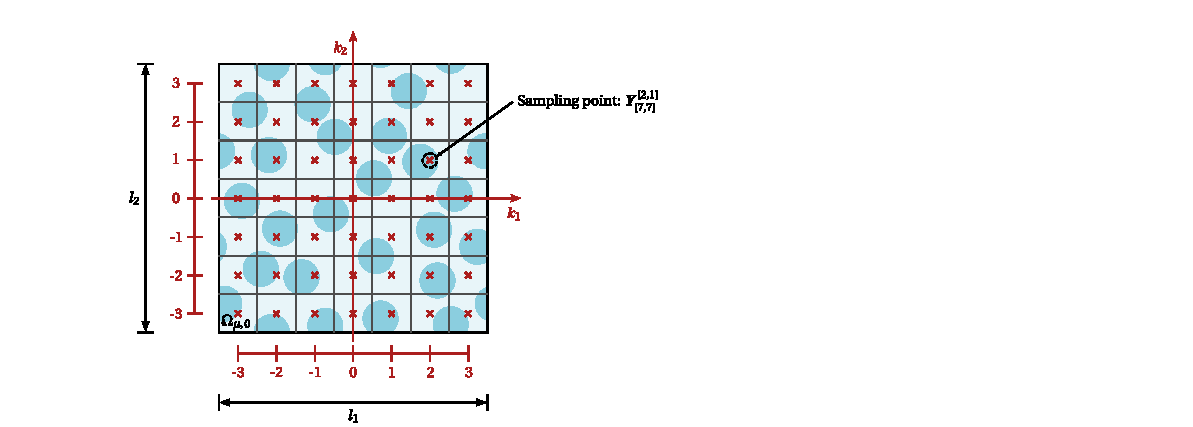
\includegraphics{figures/fft_discretization}
  \caption{Discretization of the periodic cell \(\Omega_{\mu,0}\) with \(\bm n_v = [7,7]\) to be used in the FFT-based homogenization procedure.}
\label{fig:fft_discretization}
\end{figure}

As explained below, only grids with an odd number of nodes will be considered.
For the extension to even grids see Appendix~\ref{app:fft}.
The individual nodes are indexed by a parameter \(\bm k\) from a reduced index set
\begin{equation}
\mathbb{Z}_{\bm n_v}^{d}=\left\{\bm{ k} \in \mathbb{Z}^{d}\ |\ \forall i \in [1,d]\cap \mathbb Z \left(-\frac{n_{v,i}}{2}< k_{i}<\frac{n_{v,i}}{2}\right) \right\}\quad \text{with \(d=2\) or 3},
\end{equation}
and it will become clear later that the indices \(\bm  k\) can be naturally identified with the discrete frequencies from \eqref{eq:compatibility_equations}.
Finally, the integration weight \(w=v_{\mu,0} /n_v\) is set equal to the pixel/voxel size, corresponding to each node.

It is convenient to use the {fundamental trigonometric polynomials} defined on the grid \(\mathbb{Z}_{\bm n_v}^{d}\),
\begin{equation}\label{eq:fundamental_trigonometric_polynomials}
\varphi_{\bm n_v}^{\bm k}(\bm{Y})=\frac{1}{n_v} \sum_{\bm{ m} \in \mathbb{Z}_{\bm n_v}^{d}} \omega_{\bm n_v}^{-\bm{ k  m}} \varphi^{\bm  m}(\bm{ Y})\quad \text { for } \bm{ k} \in \mathbb{Z}_{\bm n_v}^{d},
\end{equation}
as the basis functions to approximate the weak form in Equation~\eqref{eq:form_to_be_discretized}.
Here, \(\varphi^{\bm  m}\) stands for the Fourier basis function (Equation~\eqref{eq:fourier_basis_functions})) and \(\omega_{\bm n_v}^{\bm  k \bm m}\) are the complex-valued coefficients of the Discrete Fourier Transform (DFT),
\begin{equation} \label{eq:def_dft_coefficients}
\omega_{\bm n_v}^{\bm  k \bm  m}=\omega_{\bm n_v}^{\bm  m\bm  k}=\varphi^{\bm  k}\left(\bm Y_{\bm n_v}^{\bm  m}\right)=\exp \left(\mathrm{i}\bm Y_{\bm n_v}^{\bm  k}\cdot \bm \zeta (\bm m)\right) \text { for } \bm{ k}, \bm{ m} \in \mathbb{Z}_{\bm n_v}^{d}.
\end{equation}

The solution \(\tilde{\bm\varepsilon}_\mu\) and the test functions \(\bm \xi\) in Equation~\eqref{eq:convolution_projection_operator} will be approximated as a linear combination of the basis functions \(\varphi_{\bm n_v}^{\bm  k}\); the corresponding approximation space of the tensor-valued trigonometric polynomials will be referred to as \(\pazocal{T}_{\bm n_v}\).
These approximations are conforming, i.e., \(\pazocal{T}_{\bm n_v} \subset \pazocal{H}\), as long as the number of nodes \(n_v\) is odd.
This conformity is lost when \(n_v\) is even, resulting in a more elaborate treatment.

The computational convenience of trigonometric polynomials follows from the fact that they can be efficiently manipulated using the Fast Fourier Transform (FFT), because of (i) the involvement of the DFT coefficients \(\omega_{\bm n_v}^{\bm  k\bm  m}\) in Equation~\eqref{eq:fundamental_trigonometric_polynomials} and (ii) the ability to work with quantities defined in the Fourier space, because they incorporate the Fourier basis functions \(\varphi^{\bm m}\).

In what follows, the most important steps needed to discretize the weak form in Equation~\eqref{eq:weak_form_equilibrium_eq} are collected.

As can be seen from the example in Figure~\ref{fig:example_fundamental_polynomial}, in the real space the fundamental trigonometric polynomials are not locally supported, unlike the conventional Finite Element shape functions, however they are still interpolatory and form the partition-of-unity, because they satisfy
\begin{equation} \label{eq:delta_property}
\varphi_{\bm n_v}^{\bm  k}\left(\bm   Y_{\bm n_v}^{\bm  m}\right)=\delta^{\bm  k \bm  m} \text { for } \bm  k, \bm  m \in \mathbb{Z}_{\bm n_v}^{d}, \quad \sum_{\bm  k \in \mathbb{Z}_{\bm n_v}^{2}} \varphi_{\bm n_v}^{\bm  k}(\bm Y)=1 \text { for } \bm Y \in \Omega_{\mu,0},
\end{equation}
where \(\delta^{\bm  k \bm  m}\) is the Kronecker delta.
In the Fourier domain, they are locally supported on \(\mathbb{Z}_{\bm n_v}^{d}\),
\begin{equation} \label{eq:basis_functions_compact_suppport}
\breve{\varphi}_{\bm n_v}^{\bm  k}(\bm{ m})=0\ \text { for } \bm{ k} \in \mathbb{Z}_{\bm n_v}^{d}, \bm  m \in \mathbb{Z}^{d} \backslash \mathbb{Z}_{\bm n_v}^{d},
\end{equation}
because their definition (Equation~\eqref{eq:fundamental_trigonometric_polynomials}) contains only the Fourier basis functions \(\varphi^{\bm  m}\) associated with the frequencies from the grid \(\mathbb{Z}_{\bm n_v}^{d}\).

\begin{figure}
  \centering
  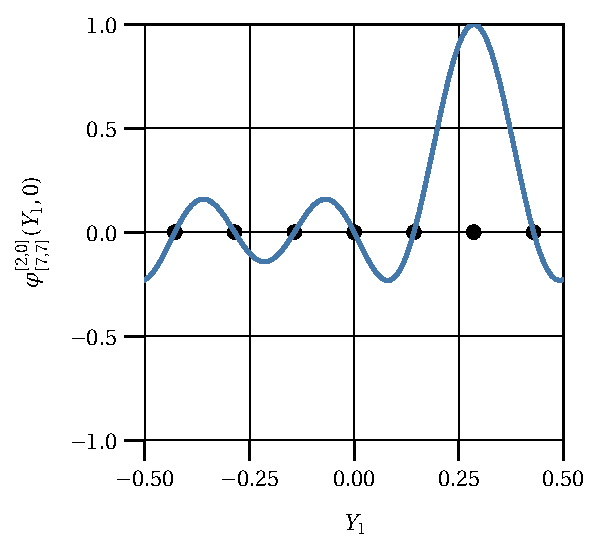
\includegraphics[width=0.55\textwidth]{figures/fundamental_trig_pol}
  \caption{Plot of the fundamental polynomial \(\varphi_{[7,7]}^{[2,0]}(\bm Y)\) for \(-0.5\leq Y_1\leq 0.5\) and \(Y_2=0\). The sampling points are shown as black markers.}
\label{fig:example_fundamental_polynomial}
\end{figure}

As a consequence, every trigonometric polynomial \(\bm\tau \in \pazocal{T}_{\bm n_v}\) admits two equivalent representations on the same grid \(\mathbb{Z}_{\bm n_v}^{d}\) that involve its nodal values \(\bm\tau\left(\bm{Y}_{\bm n_v}^{\bm{ k}}\right)\), and the Fourier coefficients \(\breve{\bm{\tau}}(\bm{ k})\).
Their mutual relation is established by the forward and inverse DFTs,
\begin{gather} \label{eq:forward_fft}
\breve{\bm\tau}(\bm{ k})=\mathcal{DFT}\big (\bm \tau\big )(\bm k)=\frac{1}{n_v} \sum_{\bm  m \in \mathbb{Z}_{\bm n_v}^{d}} \omega_{\bm n_v}^{-\bm  k \bm  m} \bm{\tau}\left(\bm{Y}_{\bm n_v}^{\bm  m}\right)\quad \text { for } \bm{ k} \in \mathbb{Z}_{\bm n_v}^{d},\\
\label{eq:backward_fft}
 \bm{\tau}\left(\bm{Y}_{\bm n_v}^{\bm{ k}}\right)=\mathcal{DFT}^{-1}\big (\breve{\bm \tau}\big )(\bm{Y}_{\bm n_v}^{\bm{ k}})=\sum_{\bm  m \in \mathbb{Z}_{\bm n_v}^{d}} \omega_{\bm n_v}^{\bm  k \bm  m} \breve{\bm{\tau}}(\bm{ m})\quad \text { for } \bm{ k} \in \mathbb{Z}_{\bm n_v}^{d}.
\end{gather}

\subsection{Numerical integration}

The scalar product of two trigonometric polynomials \(\bm\tau \in \pazocal{T}_{\bm n_v}\) and \(\bm{\theta} \in \pazocal{T}_{\bm n_v}\) can be evaluated exactly by the trapezoidal rule,
\begin{equation} \label{eq:trapezoidal_rule}
\int_{\Omega_{\mu,0}} \bm\tau(\bm Y): \bm\theta(\bm Y) \mathrm{d} v=w \sum_{\bm{ k} \in \mathbb{Z}_{\bm n_v}^{d}} \bm{\tau}\left(\bm{Y}_{\bm n_v}^{\bm k}\right): \bm{\theta}\left(\bm{Y}_{\bm n_v}^{\bm{ k}}\right),
\end{equation}
which assigns the same integration weight, equal to the pixel area \(w\), to each grid node.

\subsection{Convolution}

Convolution. of a trigonometric polynomial \(\bm\tau \in \pazocal{T}_{n_v}\) with the projection operator \(\boldsf G\) from \eqref{eq:compatibility_of_test_functions} can be evaluated efficiently at the grid nodes \(\bm Y_{\bm n_v}^{\bm  k}\) by DFT.
Accordingly, from Equation~\eqref{eq:convolution_projection_operator} one finds
\begin{equation}
[\boldsf{G} * \bm{\tau}]\left(\bm{Y}_{\bm n_v}^{\bm  k}\right) = \sum_{\bm  m \in \mathbb{Z}^{d}} \breve{\boldsf{G}}(\bm{ m}):\left[\breve{\bm{\tau}}(\bm{ m}) \varphi^{\bm  m}\left(\bm{Y}_{\bm n_v}^{\bm  k}\right)\right].
\end{equation}
Noting that in the frequency domain the basis functions have compact support (Equation~\eqref{eq:basis_functions_compact_suppport}) and applying the definition for the coefficients of the DFT (Equation~\eqref{eq:def_dft_coefficients}), yields
\begin{equation}
  \sum_{\bm  m \in \mathbb{Z}^{d}} \breve{\boldsf{G}}(\bm{ m}):\left[\breve{\bm{\tau}}(\bm{ m}) \varphi^{\bm  m}\left(\bm{Y}_{\bm n_v}^{\bm  k}\right)\right] = \sum_{\bm  m \in \mathbb{Z}_{\bm n_v}^{d}}  \breve{\boldsf{G}}(\bm{ m}):\left[\breve{\bm\tau}(\bm{ m}) \omega_{\bm n_v}^{\bm  k \bm  m}\right].
\end{equation}
Thus, from the definition of the Discrete Fourier Transform in Equation~\eqref{eq:forward_fft}, the desired result is achieved
\begin{equation}
[\boldsf{G} * \bm{\tau}]\left(\bm{Y}_{\bm n_v}^{\bm  k}\right) = \sum_{\bm  m \in \mathbb{Z}_{\bm n_v}^{d}} \omega_{\bm n_v}^{\bm  k \bm  m} \breve{\boldsf{G}}(\bm{ m}):\left[\frac{1}{n_v} \sum_{\bm  n \in \mathbb{Z}_{\bm n_v}^{d}}
\omega_{\bm n_v}^{-\bm  m \bm  n} \bm{\tau}\left(\bm{Y}_{\bm n_v}^{\bm  n}\right)\right],
\end{equation}
which can be written in a more compact form as
\begin{equation} \label{eq:main_computation_short}
[\boldsf{G} * \bm{\tau}]\left(\bm{Y}_{\bm n_v}^{\bm  k}\right)= \mathcal{DFT}^{-1}\left(\tilde{\boldsf G}:\mathcal{DFT}\left(\bm \tau\right)\right)\left(\bm{Y}_{\bm n_v}^{\bm  k}\right).
\end{equation}

For the non-zero frequency \(\bm k \in \mathbb{Z}_{\bm n_v}^{d} \backslash\{\bm 0\}\), the Fourier transform of the fourth-order projection operator \(\breve{\boldsf G}\) is provided by
\begin{equation} \label{eq:projection_operator_small_strains}
\begin{aligned}
\breve{\boldsf G}_{i j l m}(\boldsymbol{k})=& \frac{1}{2} \frac{\zeta_{i}(\boldsymbol{k}) \delta_{j l} \zeta_{m}(\boldsymbol{k})+\zeta_{i}(\boldsymbol{k}) \delta_{j m} \zeta_{l}(\boldsymbol{k})+\zeta_{j}(\boldsymbol{k}) \delta_{i l} \zeta_{m}(\boldsymbol{k})+\zeta_{j}(\boldsymbol{k}) \delta_{i m} \zeta_{l}(\boldsymbol{k})}{\|\boldsymbol{\zeta}(\boldsymbol{k})\|^{2}} \\
&-\frac{\zeta_{i}(\boldsymbol{k}) \zeta_{j}(\boldsymbol{k}) \zeta_{l}(\boldsymbol{k}) \zeta_{m}(\boldsymbol{k})}{\|\boldsymbol{\zeta}(\boldsymbol{k})\|^{4}},
\end{aligned}
\end{equation}
where \(\zeta_{i}\) are the scaled frequencies and \(\delta_{i j}\) stands for the Kronecker delta.
For \(\boldsymbol{k}=\mathbf{0}\), \(\breve{\boldsf G}_{i j l m}(\mathbf{0})=0\) because of the zero-mean property.

\section{Discretization}

One is now in a position to discretize the weak form of Equation~\eqref{eq:weak_form_equilibrium_eq} with trigonometric polynomials.
Following the standard Galerkin procedure, the unknown field \(\tilde{\bm \varepsilon}_\mu\) and the test field \(\bm \xi\) are approximated in the same way
\begin{align}
\tilde{\bm\varepsilon}_\mu(\bm{Y}) &\approx \sum_{\bm  m \in \mathbb{Z}_{\bm n_v}^{d}} \varphi_{\bm n_v}^{\bm  m}(\bm{Y}) \tilde{\bm \varepsilon}_\mu \left(\bm Y_{\bm n_v}^{\bm  m}\right), \\
\bm \xi(\bm{Y}) &\approx \sum_{\bm  m \in \mathbb{Z}_{\bm n_v}^{d}} \varphi_{\bm n_v}^{\bm m}(\bm{Y}) \bm \xi\left(\bm{Y}_{\bm n_v}^{\bm  m}\right).
\end{align}

The nodal strains, \(\tilde{\bm\varepsilon}_\mu\left(\bm Y_{\bm n_v}^{\bm  m}\right)\) for \(\bm m\in \mathbb Z^d_{\bm n_v}\), and the nodal values of test fields, \(\bm \xi\left(\bm Y_{\bm n_v}^{\bm  m}\right)\) for \(\bm m\in \mathbb Z^d_{\bm n_v}\), are respectively located in the corresponding finite-dimensional spaces \(\mathbb{E}_{\bm n_v} \subset \mathbb{T}_{\bm n_v}\).
The (constrained) space \(\mathbb{E}_{\bm n_v}\) thus collects the nodal values of compatible trigonometric polynomials from \(\pazocal{T}_{\bm n_v} \cap \pazocal{E}\), whereas (unconstrained) \(\mathbb{T}_{\bm n_v}\) collects nodal values of all trigonometric polynomials from \(\pazocal{T}_{\bm n_v}\).

Introducing these expansions into Equation~\eqref{eq:form_to_be_discretized} yields
\begin{equation}
\int_{\Omega_{\mu,0}}\Big(\sum_{\bm  m \in \mathbb{Z}_{\bm n_v}^{d}} \varphi_{\bm n_v}^{\bm  m}(\bm{Y}) \bm\xi\left(\bm{Y}_{\bm n_v}^{\bm  m}\right)  \Big ):[\boldsf{G} * \bm{\sigma}_\mu]\Big(\bm{Y}, \bm{\varepsilon}(\bm X)+\sum_{\bm  m \in \mathbb{Z}_{\bm n_v}^{d}} \varphi_{\bm n_v}^{\bm  m}(\bm{Y}) \tilde{\bm \varepsilon}_\mu \left(\bm Y_{\bm n_v}^{\bm  m}\right) \Big) \mathrm{d} v=0,
\end{equation}
to be satisfied for arbitrary \(\bm\xi\left(\bm{Y}_{\bm n_v}^{\bm  m}\right)\) from \(\mathbb T_{n_v}\), \(\bm m \in \mathbb Z^d_{\bm n_v}\).
Application of the trapezoidal quadrature rule (Equation~\eqref{eq:trapezoidal_rule}) provides
\begin{equation}
w \sum_{\bm  k \in \mathbb{Z}_{\bm n_v}^{d}}\Big(\sum_{\bm  m \in \mathbb{Z}_{\bm n_v}^{d}} \varphi_{\bm n_v}^{\bm  m}(\bm Y_{\bm n_v}^{\bm  k}) \bm\xi\left(\bm{Y}_{\bm n_v}^{\bm  m}\right)\Big):[\boldsf G * \bm{\sigma}_\mu]\Big(\bm Y_{\bm n_v}^{\bm  k}, \bm \varepsilon(\bm X)+\sum_{\bm  m \in \mathbb{Z}_{\bm n_v}^{d}} \varphi_{\bm n_v}^{\bm  m}\left(\bm Y_{\bm n_v}^{\bm  k}\right) \tilde{\bm \varepsilon}_\mu \left(\bm Y_{\bm n_v}^{\bm  m}\right)\Big) \approx 0,
\end{equation}
note that this step introduces an approximation error because the constitutive relation \(\bm{\sigma}_\mu\) does not necessarily map trigonometric polynomials to trigonometric polynomials.
By exploring the Kronecker delta property of the basis functions (Equation~\eqref{eq:delta_property}), the previous relation further simplifies to
\begin{equation} \label{eq:final_variational_form}
\sum_{\bm  k \in \mathbb{Z}_{\bm n_v}^{d}} \bm\xi\left(\bm{Y}_{\bm n_v}^{\bm  k}\right):[\boldsf G * \bm\sigma_\mu]\Big(\bm Y_{\bm n_v}^{\bm k}, \bm \varepsilon(\bm X)+\tilde{\bm \varepsilon}_\mu \left(\bm Y_{\bm n_v}^{\bm  k}\right)\Big)=0.
\end{equation}

Because the test strains \(\bm \xi(\bm Y_{\bm n_v}^{\bm k})\), for \(\bm k\in \mathbb Z^{d}_{\bm n_v}\), are arbitrary, one finally obtains from \eqref{eq:final_variational_form} that the nodal strain values, \(\tilde{\bm\varepsilon}_\mu(\bm Y_{\bm n_v}^{\bm k}) \in \mathbb{E}_{\bm n_v}\), for \(\bm k\in \mathbb Z^{d}_{\bm n_v}\), follow from the system of non-linear nodal equilibrium conditions,
\begin{equation} \label{eq:final_form_sum}
[\boldsf G * \bm\sigma_\mu]\Big(\bm Y_{\bm n_v}^{\bm k}, \bm \varepsilon(\bm X)+\tilde{\bm \varepsilon}_\mu \left(\bm Y_{\bm n_v}^{\bm  k}\right)\Big)=\bm 0\quad \text{for \( \bm k \in \mathbb Z^d_{\bm n_v}\)},
\end{equation}
which can be also be written as
\begin{equation} \label{eq:non_linear_equilibrium_equations}
\mathcal{DFT}^{-1}\left(\tilde{\boldsf G}:\mathcal{DFT}\left(\bm \sigma_\mu\right)\right)\left(\bm{Y}_{\bm n_v}^{\bm  k}, \bm \varepsilon(\bm X)+\tilde{\bm \varepsilon}_\mu \left(\bm Y_{\bm n_v}^{\bm  k}\right)\right)= \bm 0\quad \text{for \(\bm k \in \mathbb Z^d_{\bm n_v}\)}.
\end{equation}
where the non-linearity originates solely from the constitutive relation, because the projection operator \(\boldsf G\) is independent of \(\tilde{\bm\varepsilon}_\mu\).

Therefore, apart from enforcing the strain compatibility, the symmetric matrix \(\boldsf G\) also enforces the nodal equilibrium conditions.
Also notice that, in analogy to Section~\ref{sec:compatibility}, the constraint \(\tilde{\bm\varepsilon}_\mu(\bm Y_{\bm n_v}^{\bm k}) \in \mathbb{E}_{\bm n_v}\), for \(\bm k\in \mathbb Z^{d}_{\bm n_v}\), still needs to be accounted for.

\section{Linearization} \label{sec:linearization}

The conventional Newton scheme is used to find the solution to the system \eqref{eq:non_linear_equilibrium_equations} iteratively. For this purpose, we express the nodal unknowns in the \((i+1)\)-th iteration as
\begin{equation}
\tilde{\bm\varepsilon}_{\mu}^{(i+1)}\left(\bm{Y}_{\bm n_v}^{\bm  k}\right) =\tilde{\bm\varepsilon}_{\mu}^{(i)}\left(\bm{Y}_{\bm n_v}^{\bm  k}\right)+\delta \tilde{\bm\varepsilon}_{\mu}\left(\bm{Y}_{\bm n_v}^{\bm  k}\right)\quad \text{for \(\bm k \in \mathbb Z^d_{\bm n_v}\)}.
\end{equation}
Equation~\eqref{eq:non_linear_equilibrium_equations} is then linearized around \(\tilde{\bm\varepsilon}_\mu^{(i)}\), with \(\tilde{\bm\varepsilon}_\mu^{(0)}\left(\bm{Y}_{\bm n_v}^{\bm  k}\right) \in \mathbb{E}_{\bm n_v}\), for \(\bm k\in \mathbb Z^{d}_{\bm n_v}\).
As a result, one obtains the linear system for the nodal strain increment \(\delta \tilde{\bm\varepsilon}_\mu\left(\bm{Y}_{\bm n_v}^{\bm  k}\right) \in \mathbb{E}_{\bm n_v}\), for \(\bm k\in \mathbb Z^{d}_{\bm n_v}\),
\begin{multline} \label{eq:linearized_equilibrium_equations}
[\boldsf G * \boldsf D^{(i)}]\left(\bm{Y}_{\bm n_v}^{\bm  k}, \bm \varepsilon(\bm X)+\tilde{\bm \varepsilon}_\mu \left(\bm Y_{\bm n_v}^{\bm  k}\right)\right)\delta \tilde{\bm\varepsilon}_{\mu}^{(i+1)}\left(\bm{Y}_{\bm n_v}^{\bm  k}\right)\\ = -[\boldsf G * \bm\sigma_\mu]\left(\bm{Y}_{\bm n_v}^{\bm  k}, \bm \varepsilon(\bm X)+\tilde{\bm \varepsilon}_\mu \left(\bm Y_{\bm n_v}^{\bm  k}\right)\right)\quad \text{for \(\bm k \in \mathbb Z^d_{\bm n_v}\)},
\end{multline}
where the local tangent matrix \(\boldsf D^{(i)}\) is given by
\begin{equation}
\boldsf D^{(i)}\left(\bm{Y}_{\bm n_v}^{\bm  k}, \bm \varepsilon(\bm X)+\tilde{\bm \varepsilon}_\mu \left(\bm Y_{\bm n_v}^{\bm  k}\right)\right)=\frac{\partial \bm{\sigma}_\mu}{\partial \bm \varepsilon_\mu}\left(\bm{Y}_{\bm n_v}^{\bm  k}, \bm \varepsilon(\bm X)+\tilde{\bm \varepsilon}_\mu \left(\bm Y_{\bm n_v}^{\bm  k}\right)\right) \text { for } \bm  k \in \mathbb{Z}_{\bm n_v}^{d}.
\end{equation}

Three considerations must be taken into account when solving the linearized system (Equation~\eqref{eq:linearized_equilibrium_equations}):
\begin{enumerate}[(i)]
  \item the corresponding system matrix is dense, singular, and very costly to assemble for large grids;
  \item the multiplication with the system matrix is cheap and does not require the matrix assembly, because it involves the multiplication with structurally sparse matrices (recall that the convolution with \(\boldsf G\) can be performed efficiently by FFT (Equation~\eqref{eq:main_computation_short}); and
  \item the solver must enforce the compatibility constraint \(\tilde{\bm \varepsilon}_\mu^{(i+1)}\left(\bm{Y}_{\bm n_v}^{\bm  k}\right) \in \mathbb{E}_{\bm n_v}\), for \(\bm k\in \mathbb Z^{d}_{\bm n_v}\).
\end{enumerate}

All these aspects invite the application of (projected) iterative solvers involving only matrix-vector products, such as specific-purpose solvers \citep{moulinec_comparison_2014}, or selected general-purpose iterative algorithms for symmetric positive systems \citep{mishra_comparative_2016}, because the operator \(\boldsf G\) enforces the compatibility and equilibrium conditions simultaneously.
Specifically, we will use the conventional Conjugate Gradient algorithm \citep{hestenes_methods_1952}, which enforces the compatibility constraint at every iteration and outperforms alternative solvers in terms of convergence rate, as demonstrated in \cite{mishra_comparative_2016}.

\section{Algorithm}

To summarize, the incremental-iterative Newton-Conjugate Gradient solver is outlined as a pseudo-algorithm in Box~\ref{box:alg_newton_cg}.
For later reference, it is emphasized that the algorithm implements two termination criteria for the Newton and the Conjugate Gradient solvers that involve the two tolerances \(\eta^{\mathrm{NW}}\) and \(\eta^{\mathrm{CG}}\), respectively.
Finally, note that the same procedure applies to history- and rate-dependent material laws, once the time-incremental stress-strain laws and consistent constitutive tangents are adopted, replacing \(\bm\sigma_\mu^{(i)}\) and \(\boldsf D^{(i)}\) in Equation~\eqref{eq:linearized_equilibrium_equations}.

\begin{framedbox}[htb]
\caption{Pseudo-code for the Newton-CG algorithm solving the equilibrium problem for non-linear behavior.}
\label{box:alg_newton_cg}
\begin{center}
\begin{minipage}{0.9\textwidth}
\begin{enumerate}[(i)]
\item Set the initial conditions: \(t=t_0\)
\item Set strain fluctuations to zero: \(\tilde{\bm \varepsilon}_\mu^{(0)}(\bm Y^{\bm k}_{\bm n_v})=\bm{0}\) for \(\bm  k \in \mathbb{Z}_{\bm n_v}^{d}\)
\item Initialize other history variables (material dependent)
\item Enter increment loop
\begin{enumerate}[(1)]
  \item Set Newton counter to zero: \(i=0\)
  \item Initialize, indicating no convergence yet: \(\delta \tilde{\bm\varepsilon}_\mu(\bm Y^{\bm k}_{\bm n_v})={\bm \infty}\) for \(\bm  k \in \mathbb{Z}_{\bm n_v}^{d}\)
  \item Enter Newton loop
  \begin{enumerate}[(a)]
    \item Compute the constitutive response (material dependent): \[\bm{\sigma}_\mu^{(i)}(\bm Y^{\bm k}_{\bm n_v})={\bm{\sigma}_\mu}\left(\bm{Y}_{\bm n_v}^{\bm  k}, \bm \varepsilon(\bm X)+\tilde{\bm \varepsilon}_\mu \left(\bm Y_{\bm n_v}^{\bm  k}\right)\right)\quad\text{for \(\bm  k \in \mathbb{Z}_{\bm n_v}^{d}\)}\]
    \item Compute the consistent tangent (material dependent):
    \[{\boldsf D}^{(i)}(\bm Y^{\bm k}_{\bm n_v})=\frac{\partial \bm{\sigma}_\mu}{\partial \bm\varepsilon_\mu}\left(\bm{Y}_{\bm n_v}^{\bm  k}, \bm \varepsilon(\bm X)+\tilde{\bm \varepsilon}_\mu \left(\bm Y_{\bm n_v}^{\bm  k}\right)\right)\quad\text{for \(\bm  k \in \mathbb{Z}_{\bm n_v}^{d}\)}\]
    \item Use the standard Conjugate Gradient method to solve
    \[
[\boldsf G * \boldsf D^{(i)}]\left(\bm{Y}_{\bm n_v}^{\bm  k}\right)\delta \tilde{\bm\varepsilon}_{\mu}\left(\bm{Y}_{\bm n_v}^{\bm  k}\right) = -[\boldsf G * \bm\sigma_\mu^{(i)}]\left(\bm{Y}_{\bm n_v}^{\bm  k}\right)\quad \text{for \(\bm k \in \mathbb Z^d_{\bm n_v}\)}
\]
until the desired accuracy \(\eta^{CG}\) is reached.
  \item Update the strain: \({\tilde{\bm\varepsilon}_\mu}^{(i+1)}\left(\bm{Y}_{\bm n_v}^{\bm  k}\right)={\tilde{\bm\varepsilon}_\mu}^{(i)}\left(\bm{Y}_{\bm n_v}^{\bm  k}\right)+\delta {\tilde{\bm\varepsilon}_\mu}\left(\bm{Y}_{\bm n_v}^{\bm  k}\right)\)
  \item If the desired accuracy \(\eta^{\mathrm{NW}}\) has not been reached, update \(i=i+1\) and go to step (a).
  \end{enumerate}
\item Set the "intial guess" for the next increment: \({\tilde{\bm\varepsilon}_\mu}^{(t+\Delta t)}\left(\bm{Y}_{\bm n_v}^{\bm  k}\right)={\tilde{\bm\varepsilon}_\mu}^{(i)}\left(\bm{Y}_{\bm n_v}^{\bm  k}\right)\)
\item Update other history variables (material dependent)
\item If \(t\leq T_0\), proceed to next increment \(t=t+\Delta t\) and go to step (1).
\end{enumerate}
\end{enumerate}
\end{minipage}
\end{center}
\end{framedbox}


\section{Extension to finite strain}

This section presents the adaptations needed to extend the scheme introduced above to finite strains.

\subsection{Problem statement}

The goal is again to solve for the static mechanical equilibrium in the periodic cell for a given applied overall deformation.
The balance of linear momentum, pulled-back to the (undeformed) reference configuration, reads
\begin{equation} \label{eq:equilibrium_equation_finite_strain}
\operatorname{div}_0 \bm{P}_\mu=\bm{0}
\end{equation}
involving the divergence with respect to the reference configuration of the transposed first Piola-Kirchhoff stress tensor \(\bm{P}_\mu\).
The stress \(\bm{P}_\mu\) depends non-linearly on the deformation gradient \(\bm{F}_\mu\)
\begin{equation} \label{eq:constitutive_law_finite_strains}
\bm{P}_\mu=\bm{P}_\mu(\bm{F}_\mu).
\end{equation}

\subsection{Weak form}

The integral form is obtained by multiplying \eqref{eq:equilibrium_equation_finite_strain} with test functions \(\delta \bm Y\) and integrating over the reference domain \(\Omega_{\mu,0}\)
\begin{equation}
\int_{\Omega_{\mu,0}} \delta \bm Y \cdot\left(\operatorname{div}_0 \bm{P}_\mu\right) \mathrm{d} v=0,
\end{equation}
which must hold for all periodic \(\delta \bm Y\).
Subsequently, integration by parts is applied in conjunction with Gauss' divergence theorem.
The boundary term that arises vanishes because of periodicity.
The result reads
\begin{equation} \label{eq:weak_form_displacements}
\int_{\Omega_{\mu,0}}\bm{P}_\mu:\left(\operatorname{div}_0 \left(\delta \bm Y\right)\right) \mathrm{d} v=0,
\end{equation}
where \(:\) denotes a double tensor contraction.
To make use of the FFT-based methods, the weak form of Equation~\eqref{eq:weak_form_displacements} is accordingly reformulated using the deformation gradient \(\bm F_\mu\) as
\begin{equation} \label{eq:weak_form_finite_strain}
\int_{\Omega_{\mu,0}}  \bm{P}_\mu:\delta\bm{F}_\mu \mathrm{~d} v=0,
\end{equation}
in which the test functions \(\delta \bm{F}_\mu\) are periodic and compatible.
Note that compatibility is guaranteed when \(\delta \bm{F}_\mu\) is the gradient of a virtual position vector, as in Finite Elements, but now must be enforced as a constraint in conjunction with Equation~\eqref{eq:weak_form_finite_strain}.

\subsection{Projection to a compatible solution space}

As in the case of small strains, the compatibility of the test functions \(\delta \bm{F}_\mu\) is imposed employing a projection operator \(\boldsf{G}\) (different from the previous one).
It maps an arbitrary field \(\bar{\bm A}\) to its compatible part \(\bm A\) through
\begin{equation} \label{eq:projection_finite_strains}
\boldsf{G} * \overline{\bm{A}}=\bm{A},
\end{equation}
wherein \(*\) is the convolution operator.
The convolution can be evaluated in Fourier space as a simple, local, double tensor contraction.
Furthermore, \(\boldsf{G}\) has a simple closed-form expression in Fourier space,
\begin{equation} \label{eq:def_projection_finite_strains}
\breve{\boldsf G}_{i j l m}\left(\bm{k}\right)=\begin{cases}
0 & \text { for } \bm k=\bm{0} \\[5pt]
\displaystyle{\frac{\delta_{i m} \zeta_{j}\left(\bm{k}\right) \zeta_{l}\left(\bm{k}\right)}{\|\bm{\zeta}\|^{2}} } & \text { otherwise }
\end{cases},
\end{equation}
wherein \(\bm{k}\) is the (spatial) frequency vector and \(\zeta_{i}\) are the scaled frequencies that account for the size of the cell through \(\zeta_{i}(\bm k)=2\pi k_{i} / l_{i}\) (with \(l_{i}\) the size of the periodic cell in direction \(i\)).
Its background and interpretation are discussed in Appendix~\ref{app:fft}.

Application of Equation~\ref{eq:projection_finite_strains} to the weak form of Equation~\ref{eq:weak_form_finite_strain} results in
\begin{equation} \label{eq:finite_strain_eq_to_discretize}
\int_{\Omega_{\mu,0}}(\boldsf{G} * \delta \bar{\bm{F}}_\mu): \bm{P}_\mu^{T} \mathrm{d} v=\int_{\Omega_{\mu,0}} \delta \bar{\bm{F}}_\mu:(\boldsf{G} * \bm{P}_\mu) \mathrm{d} v = 0,
\end{equation}
whereby the symmetry of \(\boldsf{G}\) has been used. Equation~\eqref{eq:finite_strain_eq_to_discretize} should now hold for arbitrary, i.e. not necessarily compatible, periodic test functions \(\delta \bar{\bm{F}}_\mu\).
Please note that the deformation gradient \(\bm{F}_\mu\), hidden in the stress \(\bm{P}_\mu\) through Equation~\eqref{eq:constitutive_law_finite_strains}, should still satisfy the compatibility constraint.

\subsection{Discretization}

Adopting a Galerkin scheme, the unknown field \(\bm{F}_\mu\) and the test functions \(\delta \bar{\bm{F}}_\mu\) are discretized in the same way.
Like in Finite Elements, the continuous fields \(\bm{F}_\mu\) and \(\delta \bar{\bm{F}}_\mu\) are approximated by a finite number of \(n\) nodal values that are multiplied with shape functions associated with each node, i.e.
\begin{gather}
\bm{F}_\mu(\bm Y)  \approx \sum_{\bm m\in\mathbb{Z}^d_{\bm n_v} } \varphi_{\bm n_v}^{\bm m}(\bm Y) \bm{F}_\mu (\bm Y^{\bm m}_{\bm n_v}), \\
\delta \bar{\bm{F}}_\mu(\bm Y) \approx \sum_{\bm m\in\mathbb{Z}^d_{\bm n_v} } \varphi_{\bm n_v}^{\bm m}(\bm Y) \bar{\bm{F}}_\mu (\bm Y^{\bm m}_{\bm n_v}).
\end{gather}
Just as before, the fundamental trigonometric polynomials are used as shape functions.

The discretization is applied to the weak form (Equation~\eqref{eq:finite_strain_eq_to_discretize}) which therefore becomes
\begin{equation} \label{eq:finite_strains_final_variational}
\int_{\Omega_{\mu,0}} \Big(\sum_{\bm m\in\mathbb{Z}^d_{\bm n_v} } \varphi_{\bm n_v}^{\bm m}(\bm Y) \bar{\bm{F}}_\mu (\bm Y^{\bm m}_{\bm n_v})\Big):[\boldsf{G} * \bm{P}_\mu]\Big(\bm Y^{\bm k}_{n_v}, \sum_{\bm m\in\mathbb{Z}^d_{\bm n_v} } \varphi_{\bm n_v}^{\bm m}(\bm Y) \bm{F}_\mu (\bm Y^{\bm m}_{\bm n_v})\Big) \mathrm{d} v=0.
\end{equation}

\subsection{Quadrature}

The integration is again performed using the trapezoidal rule, which applied to Equation~\eqref{eq:finite_strains_final_variational} yields
\begin{equation}
w\sum_{\bm k\in\mathbb{Z}^d_{n_v}} \left(\left(\sum_{\bm m\in\mathbb{Z}^d_{n_v} } \varphi_{\bm n_v}^{\bm m}(\bm Y^{\bm k}_{n_v}) \bar{\bm{F}}_\mu (\bm Y^{\bm m}_{\bm n_v})\right):[\boldsf{G} * \bm{P}_\mu]\left(\bm Y^{\bm k}_{n_v},\sum_{\bm m\in\mathbb{Z}^d_{n_v} } \varphi_{\bm n_v}^{\bm m}(\bm Y^{\bm k}_{n_v}) \bm{F}_\mu (\bm Y^{\bm m}_{\bm n_v})\right)\right)\approx 0.
\end{equation}
The fact that the shape functions can be expressed in terms of the discrete Fourier coefficients is now exploited; and the delta property of the shape functions (Equation~\eqref{eq:delta_property}), writing
\begin{equation} \label{eq:final_form_sum_finite_strain}
\sum_{\bm  k \in \mathbb{Z}_{\bm n_v}^{d}} \bar{\bm{F}}_\mu (\bm Y^{\bm k}_{\bm n_v}):[\boldsf G * \bm P_\mu]\Big(\bm Y_{\bm n_v}^{\bm k}, \bm{F}_\mu (\bm Y^{\bm k}_{\bm n_v})\Big)=0.
\end{equation}

Because the test functions, \(\bar{\bm F}_\mu(\bm Y_{\bm n_v}^{\bm k})\), for \(\bm k\in \mathbb Z^{d}_{\bm n_v}\), are arbitrary, one finally obtains from \eqref{eq:final_form_sum_finite_strain} that the nodal strain values, \({\bm F}_\mu(\bm Y_{\bm n_v}^{\bm k})\), for \(\bm k\in \mathbb Z^{d}_{\bm n_v}\), follow from the system of non-linear nodal equilibrium conditions,
\begin{equation} \label{eq:final_form_sum}
[\boldsf G * \bm P_\mu]\Big(\bm Y_{\bm n_v}^{\bm k}, \bm F_\mu\left(\bm Y_{\bm n_v}^{\bm  k}\right)\Big)=\bm 0\quad \text{for \( \bm k \in \mathbb Z^d_{\bm n_v}\)},
\end{equation}
which can be also be written as
\begin{equation}\label{eq:finite_strain_final_non_lin_eq}
\mathcal{DFT}^{-1}\left(\tilde{\boldsf G}:\mathcal{DFT}\left(\bm P_\mu\right)\right)\left(\bm{Y}_{\bm n_v}^{\bm  k}, \bm F_\mu\left(\bm Y_{\bm n_v}^{\bm  k}\right)\right)= \bm 0\quad \text{for \(\bm k \in \mathbb Z^d_{\bm n_v}\)}.
\end{equation}
where the non-linearity originates solely from the constitutive relation, because the projection operator \(\boldsf G\) is independent of \(\bm F_\mu\).

Therefore, apart from enforcing the strain compatibility, the symmetric matrix \(\boldsf G\) also enforces the nodal equilibrium conditions.
Also notice, that once more, the constraint regarding the compatibility of \(\bm F_\mu\), still needs to be accounted for.

The weak form in Equation~\eqref{eq:finite_strain_final_non_lin_eq} is a non-linear equation, as the material model involves a non-linear relation between the first Piola-Kirchhoff stress and the deformation gradient.
Newton iterations are employed to solve the nodal equilibrium equations~\eqref{eq:finite_strain_final_non_lin_eq}.
To this end the nodal unknowns at iteration \(i+1\) are expressed as
\begin{equation} \label{eq:linearization_finite_strain}
{\bm{F}_\mu}^{(i+1)}\left(\bm Y_{\bm n_v}^{\bm  k}\right)={\bm{F}_\mu}^{(i)}\left(\bm Y_{\bm n_v}^{\bm  k}\right)+\delta {\bm{F}_\mu}\left(\bm Y_{\bm n_v}^{\bm  k}\right)\quad \text{for \(\bm k\in \mathbb Z^d_{\bm n_v}\)},
\end{equation}
where \({\bm{F}_\mu}^{(i)}\) are the last known iterative values of the deformation gradients and \(\delta {\bm{F}_\mu}\) are their iterative updates.
Note that \(\delta\) is now used to indicate a small variation.
The stresses are linearized around \({\bm{F}_\mu}^{(i)}\).
In a material point this corresponds to
\begin{equation} \label{eq:newton_increment}
\delta \bm{P}_\mu=\boldsf{A}^{(i)}: \delta \bm{F}_\mu.
\end{equation}

Combined with the discretized weak form in Equation~\eqref{eq:final_form_sum}, the iterative update \(\delta {\bm{F}_\mu}\) is found by solving the following linearized system
\begin{equation} \label{eq:linear_system_finite_strain}
[\boldsf{G}* \boldsf A^{(i)}] \left(\bm Y_{\bm n_v}^{\bm  k}, \bm F_\mu^{(i)}\left(\bm Y_{\bm n_v}^{\bm  k}\right)\right):\delta {\bm{F}_\mu}\left(\bm Y_{\bm n_v}^{\bm  k}\right)=-[\boldsf{G}* \bm{P}_\mu]\left(\bm Y_{\bm n_v}^{\bm  k}, \bm F_\mu^{(i)}\left(\bm Y_{\bm n_v}^{\bm  k}\right)\right)\quad\text{for \(\bm k\in \mathbb Z^d_{\bm n_v}\)}.
\end{equation}

Note that the compatibility of the deformation gradient field still needs to be enforced.
This is done by solving the linear system of Equation~\eqref{eq:linear_system_finite_strain} using an iterative solver which delivers a compatible solution in each iteration.
To satisfy compatibility during the entire iterative process, projection-based iterative methods such as e.g. the conjugate gradient (CG) method and the generalized minimal residual method (GMRES), Chebyshev iterations, or Richardson iterations (used in the original Moulinec-Suquet algorithm \citep{moulinec_fast_1994, moulinec_fft-based_1995} can be used.
Alternatively, compatibility is satisfied only at convergence for some of the accelerated methods, such as the ones based on polarization.

\subsection{Implementation}

The numerical algorithm requires the solution of Equation \eqref{eq:finite_strain_final_non_lin_eq} in an incremental-iterative fashion.
Each increment thereby consists of Newton iterations updating the nodal deformation gradients \(\bm{F}_\mu^{(i+1)}(\bm Y^{\bm k}_{\bm n_v})\), for \(\bm k\in \mathbb Z^d_{\bm n_v}\) using Equations \eqref{eq:linearization_finite_strain}-\eqref{eq:linear_system_finite_strain} until equilibrium is satisfied up to an accuracy \(\eta^{\mathrm{NW}}\), by employing the linearized constitutive response.
The linear system in Equation~\eqref{eq:linear_system_finite_strain} is solved up to an accuracy \(\eta^{\text {CG }}\) using the conjugate gradient iterative solver.
\paragraph{Boundary conditions}

With the periodic micro-fluctuations of \(\bm{F}_\mu\) following from equilibrium and compatibility, only the macroscopic deformation or stress needs to be prescribed.
Here only a fully prescribed macroscopic deformation gradient is considered \(\bar{\bm{F}}_\mu\), as this is the easiest and the most efficient choice.

The starting point is an equilibrium state given by \({\bm{F}}_\mu^{(0)}\), to which  a macroscopic deformation gradient \(\bar{\bm{F}}_\mu\) is applied.
More specifically, we apply the difference of \(\bm{\bm{F}}\) and to the mean of \({\bm{F}}_\mu^{(0)}\)
\begin{equation}
\Delta \bar{\bm{F}}_\mu\left(\bm Y_{\bm n_v}^{\bm  k}\right)=\bar{\boldsymbol{F}}_\mu\left(\bm Y_{\bm n_v}^{\bm  k}\right)-\int_{\Omega_{\mu,0}} {\bm{F}}_\mu^{(0)}\left(\bm Y_{\bm n_v}^{\bm  k}\right) \mathrm{d} v\quad \text{for \(\bm k \in \mathbb Z^d_{\bm n_v}\)}.
\end{equation}
For the first Newton iteration, equilibrium reads
\begin{equation} \label{eq:first_equilibrium}
[\boldsf{G}* \bm {P}_\mu]\left(\bm Y_{\bm n_v}^{\bm  k},\bm{F}_\mu^{(0)}\left(\bm Y_{\bm n_v}^{\bm  k}\right)+\Delta \bar{\boldsymbol{F}}_\mu\left(\bm Y_{\bm n_v}^{\bm  k}\right)+\delta {\boldsymbol{F}}_\mu\left(\bm Y_{\bm n_v}^{\bm  k}\right)\right)=\bm{0}\quad \text{for \(\bm k \in \mathbb Z^d_{\bm n_v}\)}.
\end{equation}
Linearization of \eqref{eq:first_equilibrium} results in
\begin{multline}\label{eq:first_equilibrium_lin}
[\boldsf{G}* \boldsf{A}^{(0)}]\left(\bm Y_{\bm n_v}^{\bm  k}, \bm F_\mu^{(0)}\left(\bm Y_{\bm n_v}^{\bm  k}\right)\right): \delta \bm{F}_\mu\left(\bm Y_{\bm n_v}^{\bm  k}\right)=\\-[\boldsf{G}* \boldsf{A}^{(0)}]\left(\bm Y_{\bm n_v}^{\bm  k}, \bm F_\mu^{(0)}\left(\bm Y_{\bm n_v}^{\bm  k}\right)\right): \Delta \bar{\bm{F}}\left(\bm Y_{\bm n_v}^{\bm  k}\right)\quad \text{for \(\bm k \in \mathbb Z^d_{\bm n_v}\)},
\end{multline}
where \(\boldsf{A}^{(0)}\) is the constitutive tangent about \({\bm{F}}_\mu^{(0)}\).
Note that use has been made of the fact that \({\bm{F}}_\mu^{(0)}\) is in equilibrium, i.e. that \([\boldsf G * \bm P_\mu]\left(\bm Y_{\bm n_v}^{\bm  k}, {\bm{F}}_\mu^{(0)}\right)={\bm{0}}\).
After solving the system in Equation~\eqref{eq:first_equilibrium_lin} one sets
\begin{equation}
{\bm{F}}_\mu^{(1)}\left(\bm Y_{\bm n_v}^{\bm  k}\right)={\bm{F}}_\mu^{(0)}\left(\bm Y_{\bm n_v}^{\bm  k}\right)+\Delta \bar{\bm{F}}_\mu\left(\bm Y_{\bm n_v}^{\bm  k}\right)+\delta {\bm{F}}_\mu\left(\bm Y_{\bm n_v}^{\bm  k}\right)\quad \text{for \(\bm k \in \mathbb Z^d_{\bm n_v}\)},
\end{equation}
and proceed normally.
It is thereby important to point out that the definition of \(\boldsf{G}\) ensures that the mean
\begin{equation}
\int_{\Omega_{\mu,0}} \delta {\bm {F}} \mathrm{d} v=\boldsymbol{0}.
\end{equation}
All iterations thus satisfy the prescribed \(\bar{\bm{F}}\) exactly.
The interpretation of Equation~\eqref{eq:first_equilibrium_lin} is that, by solving the linear system, the macroscopic deformation, \(\Delta \bar{\bm{F}}\), is distributed over this microstructure using the tangent \(\boldsf{A}^{(0)}\), which contains the microstructural heterogeneity.
Equation~\eqref{eq:first_equilibrium_lin} therefore has strong similarities with the application of essential (Dirichlet) boundary conditions in the Finite Element Method.
\bigskip

Box~\ref{box:alg_newton_cg_finite_strains} presents the pseudo-code for the Newton-CG scheme used to solve the non-linear equilibrium equations at finite strains.

\begin{framedbox}[htb]
\caption{Pseudo-code for the Newton-CG algorithm solving the equilibrium problem for non-linear behavior at finite strains.}
\label{box:alg_newton_cg_finite_strains}
\begin{center}
\begin{minipage}{0.9\textwidth}
\begin{enumerate}[(i)]
\item Initialize \(\bm F_\mu^{(0)}\left(\bm Y^{(k)}_{\bm n_v}\right) = \bm I\) for \(\bm k \in \mathbb Z^d_{\bm n_v}\) and history variables
\item Enter increment loop
\begin{enumerate}[(1)]
  \item Set Newton counter to zero: \(i=0\)
  \item Enter Newton loop
  \begin{enumerate}[(a)]
    \item Compute the constitutive response (material dependent): \(\bm F_\mu^{(i)} \to \boldsf A^{(i)}, \bm P_\mu^{(i)}\)
    \item According to
    \begin{itemize}
      \item If \(i=0\) then enforce the boundary condition:\\
      Solve
      \begin{multline*}
      [\boldsf{G}* \boldsf{A}^{(0)}]\left(\bm Y_{\bm n_v}^{\bm  k}, \bm F_\mu^{(0)}\left(\bm Y_{\bm n_v}^{\bm  k}\right)\right): \delta \bm{F}_\mu\left(\bm Y_{\bm n_v}^{\bm  k}\right)=\\-[\boldsf{G}* \boldsf{A}^{(0)}]\left(\bm Y_{\bm n_v}^{\bm  k}, \bm F_\mu^{(0)}\left(\bm Y_{\bm n_v}^{\bm  k}\right)\right): \Delta \bar{\bm{F}}\left(\bm Y_{\bm n_v}^{\bm  k}\right)\quad \text{for \(\bm k \in \mathbb Z^d_{\bm n_v}\)},
      \end{multline*}
      \begin{equation*}
      {\bm{F}}_\mu^{(1)}\left(\bm Y_{\bm n_v}^{\bm  k}\right)={\bm{F}}_\mu^{(0)}\left(\bm Y_{\bm n_v}^{\bm  k}\right)+\Delta \bar{\bm{F}}_\mu\left(\bm Y_{\bm n_v}^{\bm  k}\right)+\delta {\bm{F}}_\mu\left(\bm Y_{\bm n_v}^{\bm  k}\right)\quad \text{for \(\bm k \in \mathbb Z^d_{\bm n_v}\)},
      \end{equation*}
      \item else, enforce the equilibrium iteration
      \begin{multline*}
      [\boldsf{G}* \boldsf A^{(i)}] \left(\bm Y_{\bm n_v}^{\bm  k}, \bm F_\mu^{(i)}\left(\bm Y_{\bm n_v}^{\bm  k}\right)\right):\delta {\bm{F}_\mu}\left(\bm Y_{\bm n_v}^{\bm  k}\right)= \\
      -[\boldsf{G}* \bm{P}_\mu^{(i)}]\left(\bm Y_{\bm n_v}^{\bm  k}, \bm F_\mu^{(i)}\left(\bm Y_{\bm n_v}^{\bm  k}\right)\right)\quad\text{for \(\bm k\in \mathbb Z^d_{\bm n_v}\)}.
      \end{multline*}
      \begin{equation*}
      {\bm{F}_\mu}^{(i+1)}\left(\bm Y_{\bm n_v}^{\bm  k}\right)={\bm{F}_\mu}^{(i)}\left(\bm Y_{\bm n_v}^{\bm  k}\right)+\delta {\bm{F}_\mu}\left(\bm Y_{\bm n_v}^{\bm  k}\right)\quad \text{for \(\bm k\in \mathbb Z^d_{\bm n_v}\)},
      \end{equation*}
    \end{itemize}
    \item If the desired accuracy \(\eta^{NW}\) has not been reached, update index \(i=i+1\) and go to (a)
  \end{enumerate}
  \item Store the converged state \(\bm F^{(i+1)}\) and the history variables, set \(\bm F^{(0)}_\mu=\bm F^{(i+1)}_\mu\), and go to (1)
\end{enumerate}
\end{enumerate}
\end{minipage}
\end{center}
\end{framedbox}

\section{Convergence criteria} \label{sec:criteria}

Two different convergence criteria are considered in this work and described in what follows.
They include a criterion for the Conjugate Gradient procedure (interior loop) and a criterion for the Newton-Raphson procedure (exterior loop).
Let \(i\) and \(j\) be the current Newton and Conjugate Gradient iteration steps, respectively.

\paragraph{Criterion I}

Criterion I follows from the most common criterion for the Conjugate Gradient.
Since equilibrium is described by Equation~\eqref{eq:final_form_sum}, repeated here for clarity sake,
\begin{equation}
[\boldsf G * \bm P_\mu]\Big(\bm Y_{\bm n_v}^{\bm k}, \bm F_\mu\left(\bm Y_{\bm n_v}^{\bm  k}\right)\Big)=\bm 0\quad \text{for \( \bm k \in \mathbb Z^d_{\bm n_v}\)},
\end{equation}
the linearized version reads
\begin{equation}
[\boldsf{G}* \boldsf A^{(i)}] \left(\bm Y_{\bm n_v}^{\bm  k}, \bm F_\mu^{(i)}\left(Y_{\bm n_v}^{\bm  k}\right)\right):\delta {\bm{F}_\mu}\left(\bm Y_{\bm n_v}^{\bm  k}\right)=-[\boldsf{G}* \bm{P}_\mu]\left(\bm Y_{\bm n_v}^{\bm  k}, \bm F_\mu^{(i)}\left(Y_{\bm n_v}^{\bm  k}\right)\right)\quad\text{for \(\bm k\in \mathbb Z^d_{\bm n_v}\)}.
\end{equation}
Thus, the Conjugate Gradient will converge only when, for CG iteration \(j\), one verifies
\begin{equation}
\frac{\displaystyle{\left\|[\boldsf{G}* \boldsf{A}^{(i)}]: \delta \bm F_\mu^{(j)}+\boldsf{G}* \bm P_\mu^{(i)}\right\|}}{\displaystyle{\left\|\boldsf{G}* \bm P_\mu^{(i)}\right\|}}<\eta^{\mathrm{CG}},
\end{equation}
using as the reference value \(\boldsf G*\bm P_\mu^{(i)}\), where the arguments where droped for clarity.

Regarding the Newton-Raphson procedure, the tangent stiffness is updated and the same expression is used, now with the converged increment \(\delta \bm F\) from the CG method, such that the scheme has converged only when
\begin{equation}
\frac{\displaystyle{\left\|[\boldsf{G}* \boldsf{A}^{(i+1)}]: \delta \bm F_\mu+\boldsf{G}* \bm P_\mu^{(i)}\right\|}}{\displaystyle{\left\|\boldsf{G}* \bm P_\mu^{(i)}\right\|}}<\eta^{\mathrm{NW}}.
\end{equation}

The application of this criterion to the case of small strains is straightforward, needing only the deformation gradient the first Piola-Kirchhoff stress tensor to be replaced by the small strain tensor and the Cauchy stress tensor, respectively.

\paragraph{Criterion II}

Criterion II uses the consecutive values of the stress tensor to ascertain if each of the methods, Conjugate Gradient and Newton-Raphson, have converged.

For the Conjugate Gradient method it reads
\begin{equation}
\frac{\displaystyle{\left\|\bm P_\mu^{(i,j)}-\bm P_\mu^{(i,j+1)}\right\|}}{\displaystyle{\left\|\bm P_\mu^{(i,j+1)}\right\|}}<\eta^{\mathrm{CG}},
\end{equation}
where the \(\bm P_\mu^{(i,j+1)}\) is computed as
\begin{equation}
  \bm P_\mu^{(i,j+1)} = \bm P_\mu^{(i,j)}+ \boldsf A^{(i)}: \delta \bm F_\mu^{(j)},
\end{equation}
and the double superscript indicates the Cojugate Gradient and the Newton-Raphson iteraion.

For the Newton-Raphson procedure, the consequitve values for the stress in the current and the next iteration are used as follows
\begin{equation}
\frac{\displaystyle{\left\|\bm P_\mu^{(i+1)}-\bm P_\mu^{(i)}\right\|}}{\displaystyle{\left\|\bm P_\mu^{(i+1)}\right\|}}<\eta^{\mathrm{NW}}.
\end{equation}

\newpage\null\thispagestyle{blank}\newpage

\include{numerical_validation}
\chapter{Numerical Results - Elasticity}

In the following chapter, results pertaining to elasticity are presented.
The validation of the FFT-based Galerkin formulation is performed on elastic materials at
small strains and large strains.
At large strains two different models are considered, the Saint Venant-Kirchhoff
constitutive model and the Hencky constitutive model.

It is important to remark that all the numerical results shown in this chapter are obtained
in the same machine with the specifications provided in Table~\ref{tab:specifications}.
Unless otherwise stated, each numerical simulation is performed only with 1 CPU core.

\begin{table}[htbp]
\caption{Specifications of the numerical testing machine.}
\label{tab:specifications}
\centering
\begin{tabular}{clc}
\hline\hline & \vphantom{\Big |}Model & \(2 \times\) Intel Xeon E5-2650 v4 \\
& \vphantom{\Big |}Microarchitecture & Broadwell \\
& \vphantom{\Big |}Base/Max Frequency & \(2.20 / 2.90 \mathrm{GHz}\) \\
\multirow{2}{*} {CPU} & \vphantom{\Big |}Num. of cores/threads & \(24 / 48(2 \times 12 / 24)\) \\
& \vphantom{\Big |}Ll Cache & \(718 \mathrm{KiB}(2 \times 384 \mathrm{KiB})\) \\
& \vphantom{\Big |}L2 Cache & \(6 \mathrm{MiB}(2 \times 3 \mathrm{MiB})\) \\
& \vphantom{\Big |}L3 Cache & \(60 \mathrm{MiB}(2 \times 30 \mathrm{MiB})\) \\
& \vphantom{\Big |}Numerical features & SSE3 SSSE3 AVX2 \\
\hline \multirow{2}{*} {Memory } & \vphantom{\Big |}Capacity & \(128 \mathrm{~GB}(8 \times 16 \mathrm{~GB})\) \\
& \vphantom{\Big |}Specification & DDR4 @ \(2400 \mathrm{MHz}\) \\
\hline\hline
\end{tabular}
\end{table}

\section{Material characterization}

In order to perform several numerical applications in a systematic way, the same microstructures are considered throughout the entire chapter.
Without any loss of generality in what concerns the objectives of the following studies, two types of periodic microstructures are addressed following \cite{ferreira_accurate_2020}:

\begin{description}
  \item[2D microstructure] Fiber-reinforced composite characterized by unidirectional circular cross-section fibers (phase 2, \(f=30 \%\) ) randomly distributed and embedded in a matrix (phase 1, \(f=70 \%)\)\footnote{This type of microstructure is suitable to be modeled in plane strain conditions by considering any transversal plane
relative to the fibers direction.} - see Figure~\ref{subfig:2d_microstructure};

  \item[3D microstructure] Particle-reinforced composite characterized by spherical particles (phase 2, \(f=20 \%\) ) randomly distributed and embedded in a matrix (phase 1, \(f=80 \%)\) see Figure \ref{subfig:3d_microstructure}.
\end{description}

The assumed material properties for each phase are presented in Table~\ref{tab:mat_properties}.
At small strains, the material considered is linear elastic and at large strains, two constitutive models are considered.
The Saint Venant-Kirchhoff and Hencky constitutive models, both to be introduced next.

\begin{table}[htbp]
\caption{Material properties for both fiber-reinforced (2D) and particle-reinforced (3D) composites.}
\label{tab:mat_properties}
\centering
\begin{tabular}{cccc}
\vphantom{\Big |}Property & SI Units & Phase 1 & Phase 2 \\
\hline\hline \vphantom{\Big |}\(E\) & \(\mathrm{~Pa}\) & \(100 \times 10^{6}\) & \(500 \times 10^{6}\) \\
\(v\) & \(-\) & \(0.30\) & \(0.19\) \\
\hline\hline
\end{tabular}
\end{table}

\begin{figure}[hbt]
\centering
	\begin{subfigure}[b]{0.45\textwidth}
    \centering
    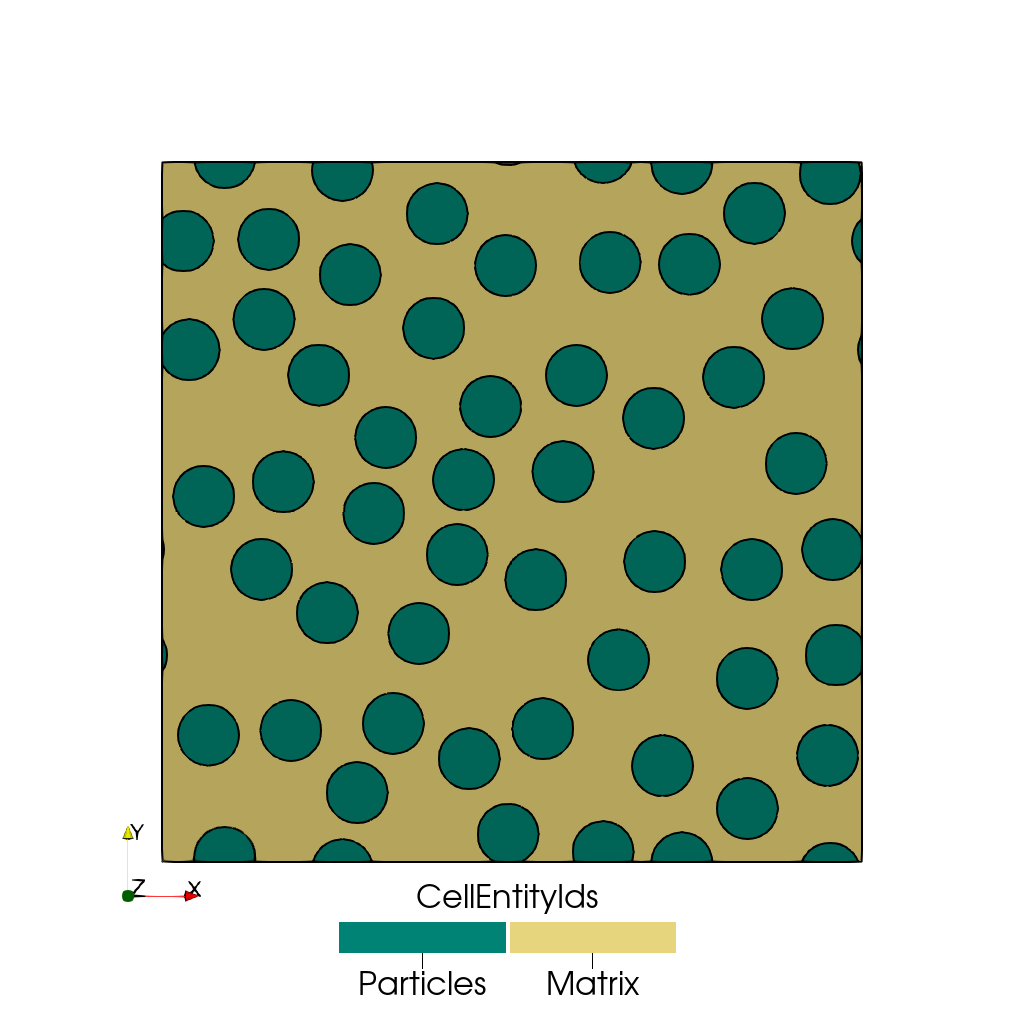
\includegraphics[width=\textwidth]{figures/2d_microstructure}
    \caption{}
    \label{subfig:2d_microstructure}
  \end{subfigure} \hfill
  \begin{subfigure}[b]{0.45\textwidth}
    \centering
    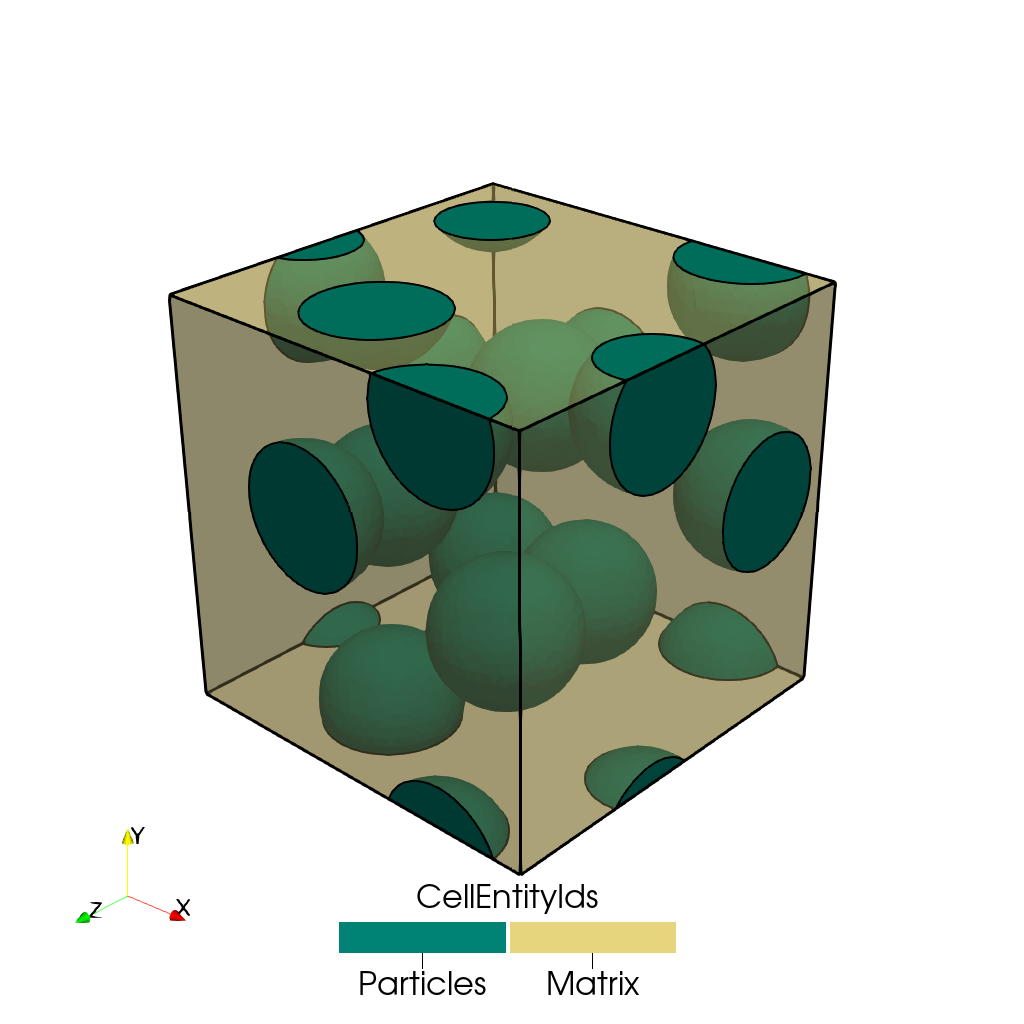
\includegraphics[width=\textwidth]{figures/3d_microstructure}
    \caption{}
    \label{subfig:3d_microstructure}
  \end{subfigure}
\caption{Dual phased heterogeneous materials microstructure: \subref{subfig:2d_microstructure} Fiber-reinforced composite (randomly distributed unidirectional circular cross-section fibers, \(f=30\%\)) - 2D RVE; \subref{subfig:3d_microstructure} Particle-reinforced composite (randomly distributed particles, \(f=20\%\)) - 3D RVE.}
\label{fig:microstructure}
\end{figure}



\subsection{Saint Venant-Kirchhoff model}

One of the simplest constitutive models to consider is a hyper-elastic model defined in the reference configuration.
Note that the problem is still non-linear because of the geometric nonlinearity.
According to \cite{de_geus_finite_2017} it can be described as follows.

\paragraph{Constitutive model}
The model is defined in the undeformed configuration and it involves a linear relation between the second Piola-Kirchhoff stress \(\boldsymbol{S}\) and the Green-Lagrange strain \(\boldsymbol{E}\)
\begin{equation} \label{eq:saint_venant_constitutive_equation}
\boldsymbol{S}=\boldsf{D}^e: \boldsymbol{E},
\end{equation}
wherein \(\boldsf{D}^e\) is the standard fourth-order elastic stiffness tensor
\begin{equation}
\boldsf{D}^e\equiv\lambda \boldsymbol{I} \otimes \boldsymbol{I}+2 \mu \boldsf{I}_{S},
\end{equation}
with Lamé's constants \(\lambda\) and \(\mu\). In terms of Young's modulus, \(E\), and Poisson's ratio, \(\nu\), they read
\begin{equation}
\lambda=\frac{E \nu}{(1+\nu)(1-2 \nu)}, \qquad \mu=\frac{E}{2(1+\nu)}.
\end{equation}
Furthermore, \(\boldsymbol{I}\) is the second-order identity tensor and \(\boldsf{I}_{S}\) is the fourth-order symmetrization tensor\footnote{The fourth order symmetrization tensor is defined as \({(\mathsf I_S)}_{ijkl} = \frac{1}{2}(\delta_{ik}\delta_{jl} + \delta_{il}\delta_{jk})\).}.

The connection to the deformation gradient tensor \(\boldsymbol{F}\) and the first Piola-Kirchhoff stress \(\boldsymbol{P}\) is made by the definition of the Green-Lagrange strain
\begin{equation}
\boldsymbol{E}=\frac{1}{2}\left(\boldsymbol{F}^{T}\boldsymbol{F}-\boldsymbol{I}\right),
\end{equation}
and of the first Piola-Kirchhoff stress
\begin{equation} \label{eq:stress_relation_saint_venant_kirchhoff}
\boldsymbol{P}=\boldsymbol{F} \boldsymbol{S}.
\end{equation}

\paragraph{Consistent tangent}
The constitutive model is linearized in the reference configuration in accordance with Equation~\eqref{eq:newton_increment}.
Its derivation is straightforward.
The first step is to linearize the stress relation in Equation~\eqref{eq:stress_relation_saint_venant_kirchhoff}, leading to
\begin{equation} \label{eq:saint_venant_kirchhoff_stress_lin}
\delta \boldsymbol{P}^{T}=\boldsymbol{S}^{(i)}\delta \boldsymbol{F}^{T}+\boldsf{I}_{R T}:\left(\boldsymbol{F}^{(i)}\delta \boldsymbol{S}\right),
\end{equation}
wherein \(\boldsf{I}_{R T}\) is the fourth-order right-transposed identity tensor\footnote{The fourth-order right-transposed identity tensor is defined as \((\mathsf I_{RT})_{ijkl} = \delta_{ik}\delta_{jl}\).}.
The constitutive model in Equation~\eqref{eq:saint_venant_constitutive_equation} is already linear.
Combined with the linearization of the Green-Lagrange strain one obtains
\begin{equation} \label{eq:saint_venant_kirchhoff_increment_2nd_piola}
\delta \boldsymbol{S}=\boldsf{D}^e:\left(\boldsf{I}^{s}{\boldsymbol{F}^{(i)}}^{T}\right): \delta \boldsymbol{F}.
\end{equation}
The expression of the tangent stiffness follows by combining Equations~\eqref{eq:saint_venant_kirchhoff_stress_lin} and \eqref{eq:saint_venant_kirchhoff_increment_2nd_piola} to obtain
\begin{equation}
\boldsf{A}^{(i)}=\boldsymbol{S}^{(i)}\boldsf{I}+\boldsf{I}_{R T}:\left(\boldsymbol{F}^{(i)}  \boldsf{D}^e  {\boldsymbol{F}^{(i)}}^{T}\right): \boldsf{I}_{R T},
\end{equation}
whereby the right-symmetry of \(\boldsf{D}^e\) has been used to absorb \(\boldsf{I}_{S}\).

\subsection{Hencky model}

The Hencky model is the finite logarithmic strain-based extension of the standard linear elastic material.
According to \cite{de2008computational} it can be described as follows.

\paragraph{Constitutive model}
Let \(\varepsilon\) be the Eulerian logarithmic strain tensor
\begin{equation} \label{eq:def_eulerian_log_strain}
\varepsilon \equiv \ln \boldsymbol{V}=\frac{1}{2} \ln \boldsymbol{B}.
\end{equation}
The Hencky strain-energy function is defined in compact form as
\begin{equation}
\bar{\rho} \psi(\varepsilon)=\frac{1}{2} \varepsilon: \boldsf{D}^e: \varepsilon,
\end{equation}
where \(\boldsf{D}^e\) has the format of the infinitesimal isotropic elasticity tensor
\begin{equation}
\boldsf{D}^e \equiv 2 G \boldsf{I}_{S}+\left(K-\frac{2}{3} G\right) \boldsymbol{I} \otimes \boldsymbol{I}.
\end{equation}

The above strain-energy renders the following linear relationship between the Kirchhoff stress and the Eulerian logarithmic strain
\begin{equation} \label{eq:hencky_stres_relation}
\bm\tau=\bar{\rho} \frac{\partial \psi}{\partial \varepsilon}=\boldsf{D}^e: \varepsilon,
\end{equation}
which has the same functional format as the infinitesimal linear elastic stress-strain relation.

\paragraph{Consistent tangent}

Under material isotropy, where \(\boldsymbol{\tau}\) can be expressed as a function of \(\boldsymbol{B}\) only, the spatial elasticity tensor can be equivalently represented as
\begin{equation} \label{eq:hecky_spatial_tangent_moduli_1st}
\boldsf{a}=\frac{2}{J} \frac{\partial \bm \tau}{\partial \bm B} \bm B-\boldsf{I}_{RT}\bm \sigma .
\end{equation}

As the Kirchhoff stress for the Hencky material is a linear function of the logarithmic Eulerian strain which, through its definition \eqref{eq:def_eulerian_log_strain}, is a function of \(B\), the derivative \(\partial \tau / \partial \boldsymbol{B}\) can be derived by a straightforward application of the chain rule to \eqref{eq:hencky_stres_relation}.
This gives
\begin{equation} \label{eq:hencky_1st_exp_for_deriv_tau_B}
\frac{\partial \boldsymbol{\tau}}{\partial \boldsymbol{B}}=\frac{\partial \boldsymbol{\tau}}{\partial \varepsilon}: \frac{\partial \varepsilon}{\partial \boldsymbol{B}}=\frac{1}{2} \boldsf{D}^e: \boldsf{L},
\end{equation}
where
\begin{equation}
\boldsf{L} \equiv \frac{\partial(\ln \boldsymbol{B})}{\partial \boldsymbol{B}},
\end{equation}
is the derivative of the tensor logarithm function evaluated at \(\bm B\).

In order to derive a compact expression for the Hencky elasticity tensor, we note that \eqref{eq:hecky_spatial_tangent_moduli_1st} is equivalent to
\begin{equation} \label{eq:hecky_spatial_tangent_moduli_2nd}
\boldsf{a}=\frac{1}{J}\frac{\partial \boldsymbol{\tau}}{\partial \boldsymbol{B}}: \boldsf{B}-\boldsf{I}_{RT}\bm\sigma
\end{equation}
where we have defined the fourth-order tensor \(\boldsf{B}\) by
\begin{equation}
\boldsf{B} \equiv 2\boldsf{I}_S \bm B.
\end{equation}
Finally, formula \eqref{eq:hecky_spatial_tangent_moduli_2nd} together with \eqref{eq:hencky_1st_exp_for_deriv_tau_B} yields the following expression for the Hencky spatial elasticity tensor
\begin{equation}
\boldsf{a}=\frac{1}{2 J}\boldsf{D}^e: \boldsf{L}: \boldsf{B}-\boldsf{I}_{RT}\bm\sigma,
\end{equation}
which has a particularly simple format.
The pull-back\textcolor{red}{(?)} to the material configuration is given by
\begin{equation}
  \boldsf{A}^{(i)} = {\bm F^{(i)}}^{-1}\left(\frac{1}{2}\boldsf{D}^e:{\boldsf L}^{(i)}: {\boldsf B}^{(i)} - \boldsf{I}_{RT}\bm \tau^{(i)}\right){\bm F^{(i)}}^{-T},
\end{equation}
reintroducing the dependency on the current Newton iteration \((i)\).

\section{Comparison between FFT and FEM-based homogenization}


To better gauge the accuracy and efficiency of the FFT-based Galerkin formulation, some numerical simulations are performed.
Their goals is to (1) validate the implementation of the FFT-based homogenization Galerkin scheme \citep{vondrejc_fft-based_2014, zeman_finite_2017, de_geus_finite_2017}, (2) compare the accuracy and computational performance between the FFT, basic \citep{moulinec_fast_1994} and Galerkin formulation, and FEM-based homogenization approaches and (3) choose the suitable spatial discretization refinement to evaluate the microstructures in Figure~\ref{fig:microstructure}.

Concerning the FFT-based homogenization, the same discretization is performed in the different problem dimensions \(\left(n_{v, 1}=n_{v, 2}=n_{v, 3}\right)\).
In order to generate the FEM finite element meshes, the FFT-FEM mesh conversion strategy adopted is to convert the pixels (2D) and voxels (3D) into quadrilateral (2D) and brick (3D) finite elements.
It is employed with both linear (QUAD4, HEXA8) and quadratic finite elements (QUAD8, HEXA20) such that \(n_{e}=n_{v}\).
Moreover, given the solver library available in LINKS, two types of solvers are considered in the FEM-based homogenization simulations: the direct solver MKL PARDISO \citep{schenk2001pardiso, schenk2004solving} and the iterative solver WSMP (Watson Sparse Matrix Package) \citep{gupta_improved_2002, gupta_wsmp_2002} with an SSOR (Symmetric Successive Over-relaxation) preconditioner.
Extensive preliminary research has shown that these are the overall (solver time and memory footprint) best direct and iterative solvers available in Links \citep{cardoso_coelho_election_2019}.

\subsection{Small strain}

\paragraph{Comparison of the convergence criteria}
The following numerical results are obtained to provide a better understanding of the differences in efficiency and accuracy between the two convergence criteria detailed in Section~\ref{sec:criteria}.

Both phases are assumed linear elastic (see Table~\ref{tab:mat_properties} for the properties), periodic boundary conditions are adopted and the following macroscale strain loading case is considered
\begin{equation}
\text { uniaxial: } \bm{\varepsilon}=\left[\begin{array}{lll}
5 & 0 & 0 \\
0 & 0 & 0 \\
0 & 0 & 0
\end{array}\right] \times 10^{-3}
\end{equation}
being enforced in a single load increment.
Note that in the 2D plane strain case, only the inplane \(O_{x y}\) macroscale strain components are enforced.

The numerical results of the fiber-reinforced linear elastic composite equilibrium problem using the two criteria under analysis are shown in Figure~\ref{fig:linear_2D_normal_comparison_crit} for the uniaxial loading case.
Figure~\ref{subfig:linear_2D_normal_comparison_crit_homo_stress_11_vs_n_voxels} shows that both FFT techniques converge to the same value at approximately the same rate as a function of the number of voxels in the discritization.
Also, no noticeable difference can be seen between the two convergence criteria considered.
Regarding the CPU time expended to reach an error of \num{1e-6}, presented in Figure~\ref{subfig:linear_2D_normal_comparison_crit_cpu_time_vs_n_voxels}, Criterion I leads to faster convergence.
This effect is stronger for the FFT Basic scheme.

\begin{figure}[hbt] % fig:linear_2D_normal_comparison_crit
  \centering
	\begin{subfigure}[b]{0.51\textwidth}
    \centering
    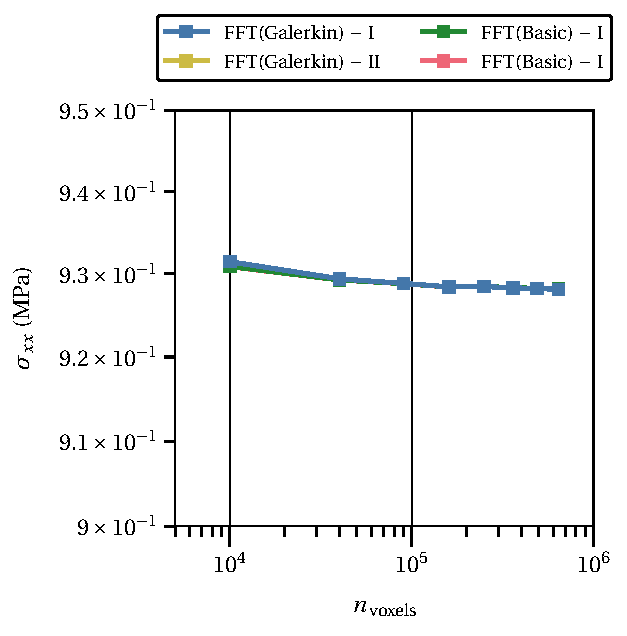
\includegraphics[width=\textwidth]{figures/linear_2D_normal_comparison_crit_homo_stress_11_vs_n_voxels}
    \caption{}
    \label{subfig:linear_2D_normal_comparison_crit_homo_stress_11_vs_n_voxels}
  \end{subfigure}
  \begin{subfigure}[b]{0.48\textwidth}
    \centering
    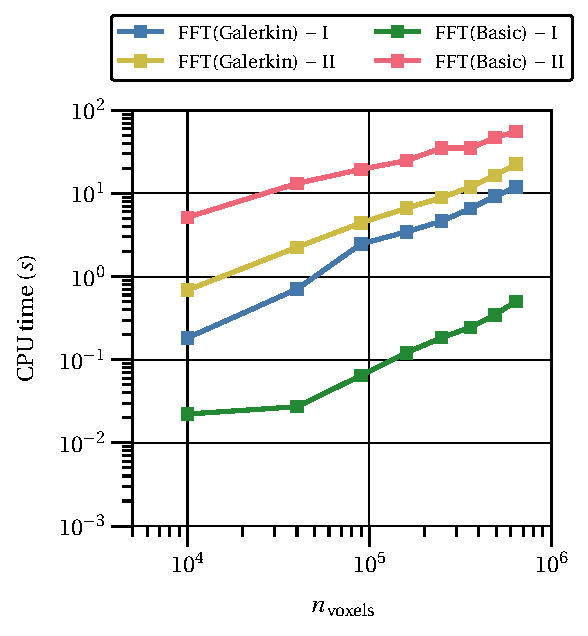
\includegraphics[width=\textwidth]{figures/linear_2D_normal_comparison_crit_cpu_time_vs_n_voxels}
    \caption{}
    \label{subfig:linear_2D_normal_comparison_crit_cpu_time_vs_n_voxels}
  \end{subfigure}
  \caption{Comparison between the Criterion I and II for FFT-based homogenization
  approaches, Galerkin and Basic, in the solution of the fiber-reinforced linear elastic
  composite equilibrium problem under uniaxial strain loading conditions:
  \subref{subfig:linear_2D_normal_comparison_crit_homo_stress_11_vs_n_voxels} Homogenized
  stress; \subref{subfig:linear_2D_normal_comparison_crit_cpu_time_vs_n_voxels}
  Computational time.}
  \label{fig:linear_2D_normal_comparison_crit}
\end{figure}

The numerical results of the particle-reinforced linear elastic composite equilibrium problem are shown in Figure~\ref{fig:linear_3D_normal_comparison_crit} for the uniaxial loading case.
The results mirror the ones found for the two-dimensional example.
Figure~\ref{subfig:linear_3D_normal_comparison_crit_homo_stress_11_vs_n_voxels} shows that both FFT techniques converge to the same value at approximately the same rate as a function of the number of voxels in the discritization.
Also, no noticeable difference can be seen between the two convergence criteria considered.
Regarding the CPU time expended to reach an error of \num{1e-5}, presented in Figure~\ref{subfig:linear_3D_normal_comparison_crit_cpu_time_vs_n_voxels}, Criterion I leads to faster convergence.
This effect is stronger for the FFT Basic scheme.

\begin{figure}[hbt] % fig:linear_3D_normal_comparison_crit
  \centering
	\begin{subfigure}[b]{0.52\textwidth}
    \centering
    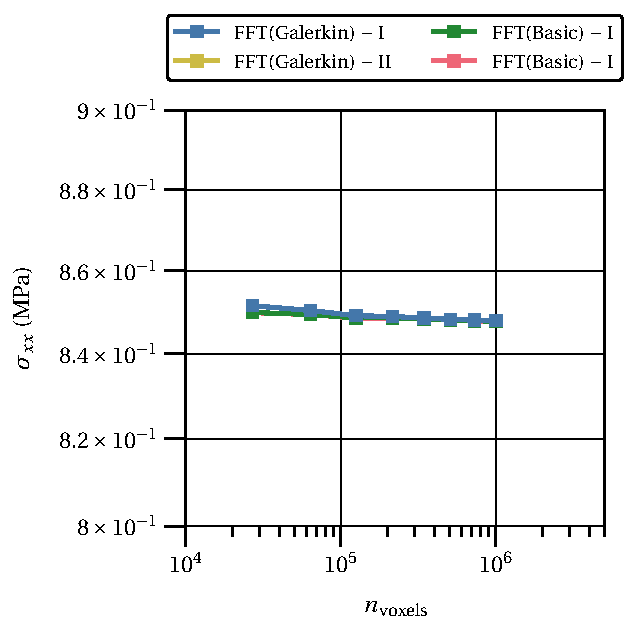
\includegraphics[width=\textwidth]{figures/linear_3D_normal_comparison_crit_homo_stress_11_vs_n_voxels}
    \caption{}
    \label{subfig:linear_3D_normal_comparison_crit_homo_stress_11_vs_n_voxels}
  \end{subfigure}
  \begin{subfigure}[b]{0.46\textwidth}
    \centering
    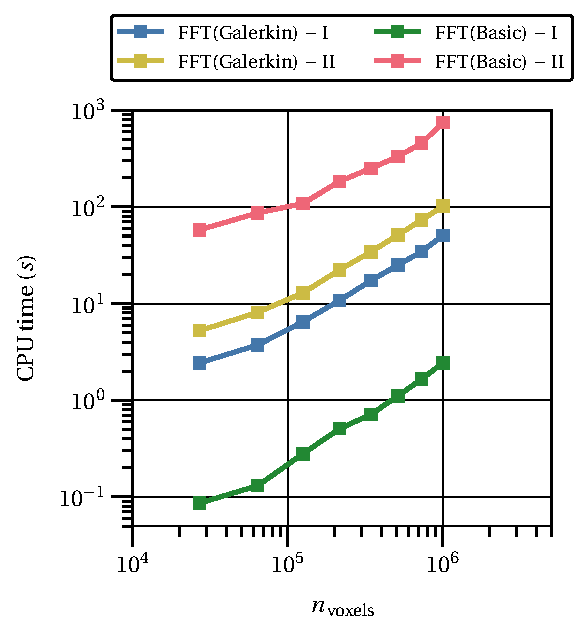
\includegraphics[width=\textwidth]{figures/linear_3D_normal_comparison_crit_cpu_time_vs_n_voxels}
    \caption{}
    \label{subfig:linear_3D_normal_comparison_crit_cpu_time_vs_n_voxels}
  \end{subfigure}
  \caption{Comparison between the Criterion I and II for FFT-based homogenization
  approaches, Galerkin and Basic, in the solution of the particle-reinforced linear elastic
  composite equilibrium problem under uniaxial strain loading conditions:
  \subref{subfig:linear_3D_normal_comparison_crit_homo_stress_11_vs_n_voxels} Homogenized
  stress; \subref{subfig:linear_3D_normal_comparison_crit_cpu_time_vs_n_voxels}
  Computational time.} \label{fig:linear_3D_normal_comparison_crit}
\end{figure}

\FloatBarrier

\paragraph{Accuracy validation}
Both phases are assumed linear elastic (see Table~\ref{tab:mat_properties} for the properties), periodic boundary conditions are adopted and the following two macroscale strain loading cases are considered
\begin{equation}
\text { uniaxial: } \bm{\varepsilon}=\left[\begin{array}{lll}
5 & 0 & 0 \\
0 & 0 & 0 \\
0 & 0 & 0
\end{array}\right] \times 10^{-3}, \quad \text { pure shear: } \quad \bm \varepsilon=\left[\begin{array}{ccc}
0 & 5 & 5 \\
5 & 0 & 5 \\
5 & 5 & 0
\end{array}\right] \times 10^{-3},
\end{equation}
being enforced in a single load increment.
Note that in the 2D plane strain case, only the inplane \(O_{x y}\) macroscale strain components are enforced.
The convergence criterion used is Criterion II, as described in Section~\ref{sec:criteria}.

The numerical results of the fiber-reinforced linear elastic composite equilibrium problem are shown in Figures~\ref{fig:linear_2D_normal} and \ref{fig:shear_2D_normal} for the uniaxial and pure shear loading cases, respectively.
In both cases there is an excellent agreement between the FFT and FEM-based homogenization solutions concerning both the homogenized response (see Figures~\ref{subfig:linear_2D_normal_homo_stress_11_vs_n_voxels} and \ref{subfig:linear_2D_shear_homo_stress_12_vs_n_voxels} and the local strain fields (see Figures \ref{subfig:linear_2D_normal_strain_11} and \ref{subfig:linear_2D_shear_strain_12}.
In terms of computational performance, Figures~\ref{subfig:linear_2D_normal_cpu_time_vs_n_voxels} and \ref{subfig:linear_2D_shear_cpu_time_vs_n_voxels} show that the FFT-based homogenization Galerkin scheme outperforms the FEM-based homogenization with speedups of around 2 relative to the direct solver with linear finite elements.
There is however a caveat, regarding this direct comparison.
The Python libraries used in the implementation of the FFT-based homogenization Galerkin scheme are parallelized and used all the cores available in the machine at the time.
On the other hand, the FEM simulations are run using only one core.
When compared with the FFT-based homogenization basic scheme, the CPU time expended differs by more than an order of magnitude, with the Galerkin scheme being slower.

\begin{figure}[hbt] % fig:linear_2D_normal
  \centering
	\begin{subfigure}[b]{0.49\textwidth}
    \centering
    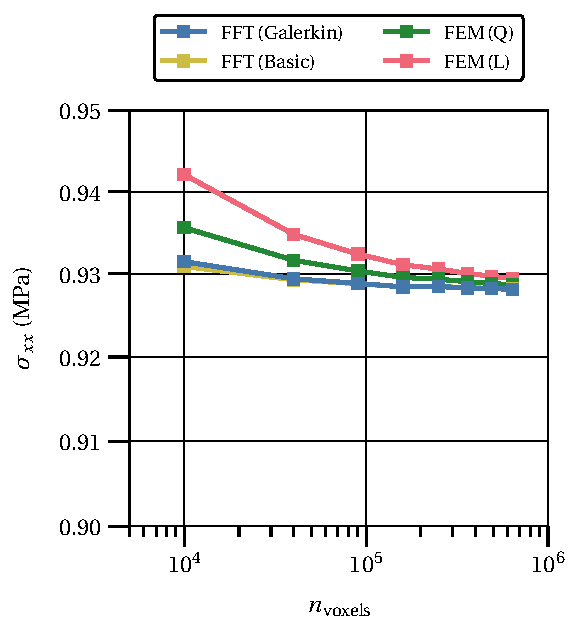
\includegraphics[width=\textwidth]{figures/linear_2D_normal_homo_stress_11_vs_n_voxels}
    \caption{}
    \label{subfig:linear_2D_normal_homo_stress_11_vs_n_voxels}
  \end{subfigure}
  \begin{subfigure}[b]{0.49\textwidth}
    \centering
    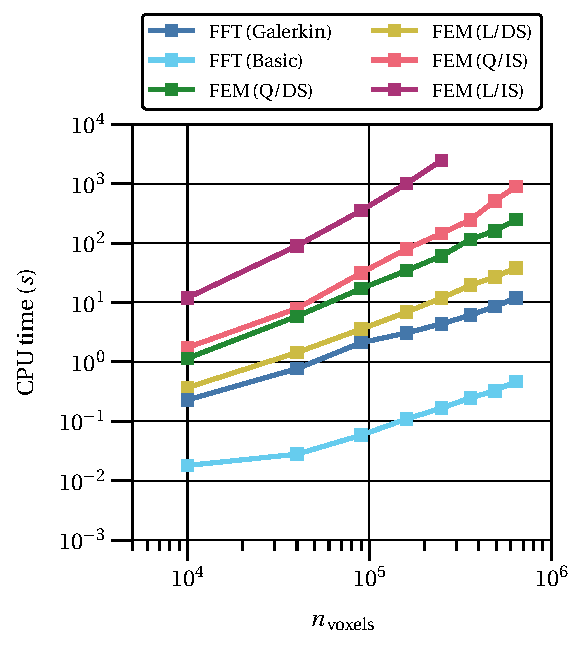
\includegraphics[width=\textwidth]{figures/linear_2D_normal_cpu_time_vs_n_voxels}
    \caption{}
    \label{subfig:linear_2D_normal_cpu_time_vs_n_voxels}
  \end{subfigure}
  \begin{subfigure}[b]{\textwidth}
    \centering
    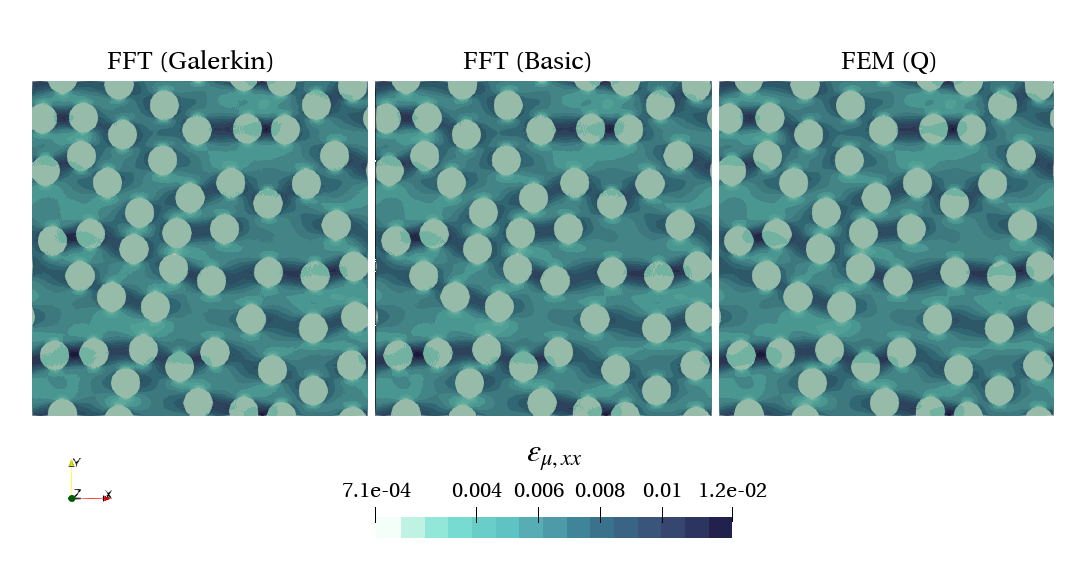
\includegraphics[width=\textwidth]{figures/linear_2D_normal_strain_11}
    \caption{}
    \label{subfig:linear_2D_normal_strain_11}
  \end{subfigure}
  \caption{Comparison between the FFT and FEM-based homogenization approaches in the
  solution of the fiber-reinforced linear elastic composite equilibrium problem under pure
  shear strain loading conditions:
  \subref{subfig:linear_2D_normal_homo_stress_11_vs_n_voxels} Homogenized stress;
  \subref{subfig:linear_2D_normal_cpu_time_vs_n_voxels} Computational time;
  \subref{subfig:linear_2D_normal_strain_11} Local strain field (\(n_v = 600 \times 600\)
  discretization). Notation: linear element (L), quadratic element (Q), direct solver (DS)
  and iterative solver (IS)}
  \label{fig:linear_2D_normal}
\end{figure}

\begin{figure}[hbt] % fig:linear_2D_shear
  \centering
	\begin{subfigure}[b]{0.49\textwidth}
    \centering
    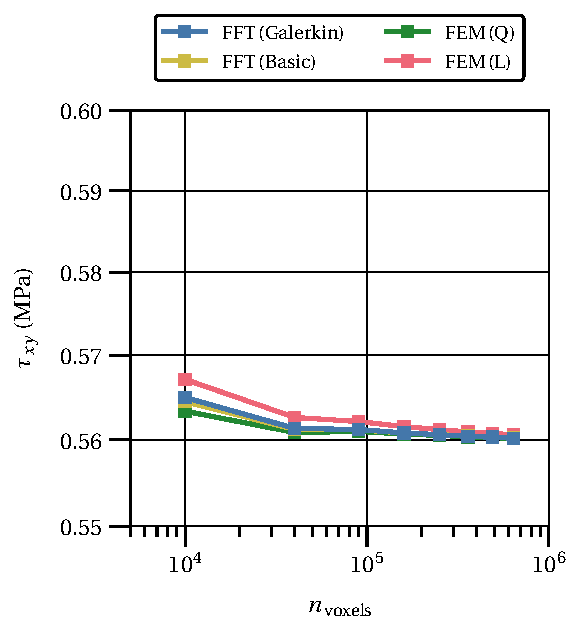
\includegraphics[width=\textwidth]{figures/linear_2D_shear_homo_stress_12_vs_n_voxels}
    \caption{}
    \label{subfig:linear_2D_shear_homo_stress_12_vs_n_voxels}
  \end{subfigure}
  \begin{subfigure}[b]{0.49\textwidth}
    \centering
    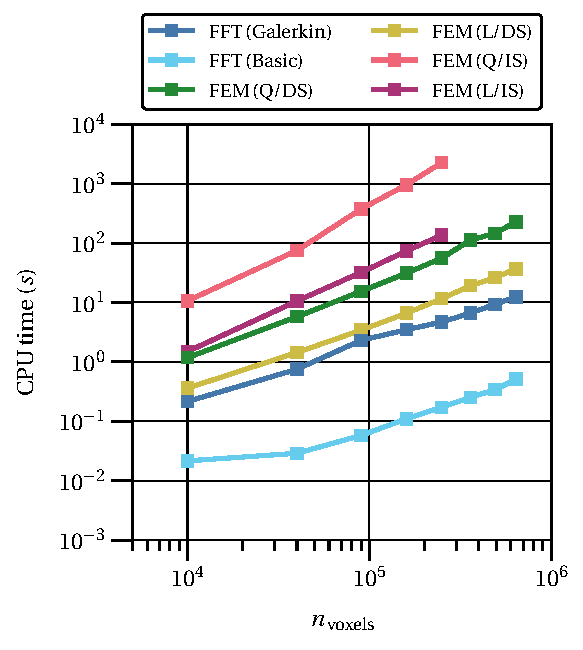
\includegraphics[width=\textwidth]{figures/linear_2D_shear_cpu_time_vs_n_voxels}
    \caption{}
    \label{subfig:linear_2D_shear_cpu_time_vs_n_voxels}
  \end{subfigure}
  \begin{subfigure}[b]{\textwidth}
    \centering
    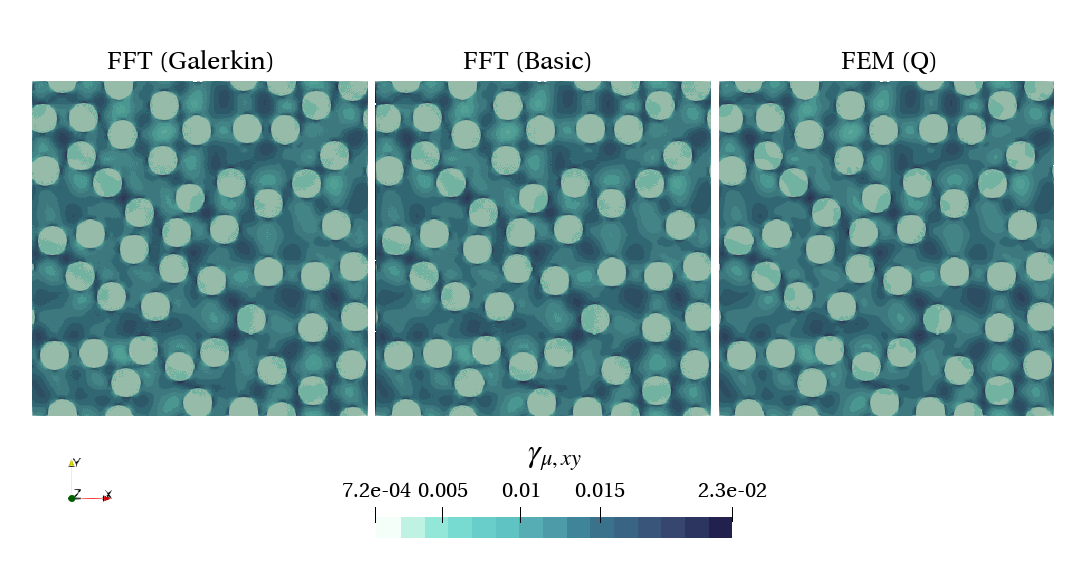
\includegraphics[width=\textwidth]{figures/linear_2D_shear_strain_12}
    \caption{}
    \label{subfig:linear_2D_shear_strain_12}
  \end{subfigure}
  \caption{Comparison between the FFT and FEM-based homogenization approaches in the
  solution of the fiber-reinforced linear elastic composite equilibrium problem under pure
  shear strain loading conditions:
  \subref{subfig:linear_2D_normal_homo_stress_11_vs_n_voxels} Homogenized stress;
  \subref{subfig:linear_2D_normal_cpu_time_vs_n_voxels} Computational time;
  \subref{subfig:linear_2D_normal_strain_11} Local strain field (\(n_v = 600 \times 600\)
  discretization). Notation: linear element (L), quadratic element (Q), direct solver (DS)
  and iterative solver (IS)}
  \label{fig:linear_2D_shear}
\end{figure}

The numerical results of the particle-reinforced linear elastic composite equilibrium problem are shown in Figures~\ref{fig:linear_3D_normal} and \ref{fig:linear_3D_shear} for the uniaxial and pure shear loading cases, respectively.
Once again there is an excellent agreement between the FFT and FEM-based homogenization solutions concerning both the homogenized response (see Figures \ref{subfig:linear_3D_normal_homo_stress_11_vs_n_voxels} and \ref{subfig:linear_3D_shear_homo_stress_12_vs_n_voxels} and the local strain fields (see Figures~\ref{subfig:linear_3D_normal_strain_11} and \ref{subfig:linear_3D_shear_strain_12}.
In terms of computational performance, Figures~\ref{subfig:linear_3D_normal_cpu_time_vs_n_voxels} and \ref{subfig:linear_3D_shear_cpu_time_vs_n_voxels} show that the FFT-based homogenization Galerkin scheme outperforms the FEM-based homogenization with speedups ranging from around 10 and 100 relative to the iterative solver with linear and quadratic finite elements, respectively.
The same remark concerning the number of cores used in each method mention previous also applies here.
Comparing the two FFT-based schemes, the basic scheme is faster by an order of magnitude than Galerkin scheme.
Adding to this, the 3D cases highlight another important aspect concerning FEM-based homogenization. When attempting to run the direct solver simulations with \(n_{e}=80 \times 80 \times 80\) (linear finite element mesh) and \(n_{e}=50 \times 50 \times 50\) (quadratic finite element mesh) the memory required to build the global tangent stiffness matrix (stored in compressed sparse row (CSR) format) exceeds the available 128 GB!
Despite reaching a significantly lower peak memory than the direct solver, the iterative solver suffered from the same limitation for a simulation over \(n_{e}=100 \times 100 \times 100\) (linear finite element mesh) and \(n_{e}=70 \times 70 \times 70\) (quadratic finite element mesh).
In comparison, the FFT-based homogenization memory footprint is almost negligible as it does not require the computation of a global tangent stiffness matrix.

\begin{figure}[hbt] % fig:linear_3D_normal
  \centering
	\begin{subfigure}[b]{0.49\textwidth}
    \centering
    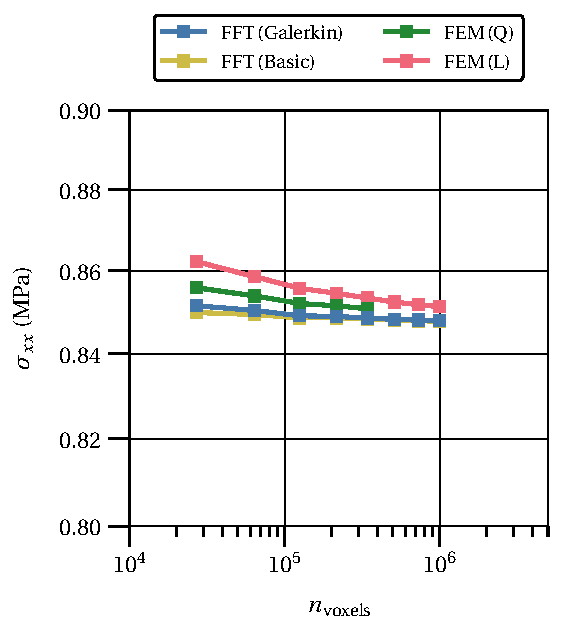
\includegraphics[width=\textwidth]{figures/linear_3D_normal_homo_stress_11_vs_n_voxels}
    \caption{}
    \label{subfig:linear_3D_normal_homo_stress_11_vs_n_voxels}
  \end{subfigure}
  \begin{subfigure}[b]{0.49\textwidth}
    \centering
    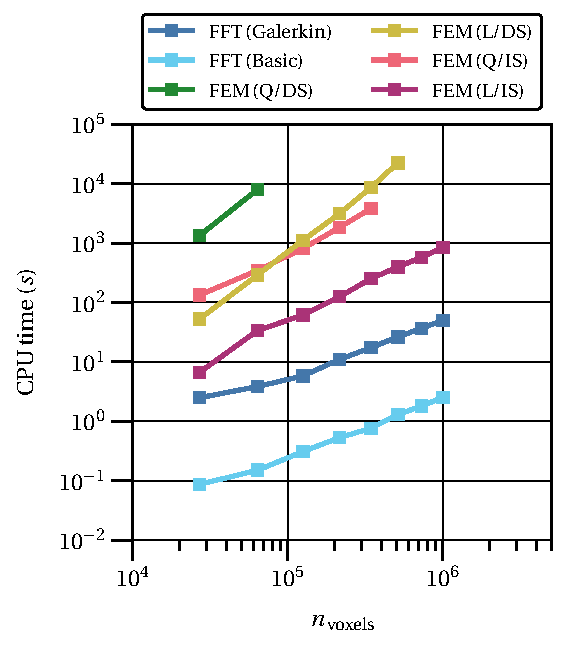
\includegraphics[width=\textwidth]{figures/linear_3D_normal_cpu_time_vs_n_voxels}
    \caption{}
    \label{subfig:linear_3D_normal_cpu_time_vs_n_voxels}
  \end{subfigure}
  \begin{subfigure}[b]{\textwidth}
    \centering
    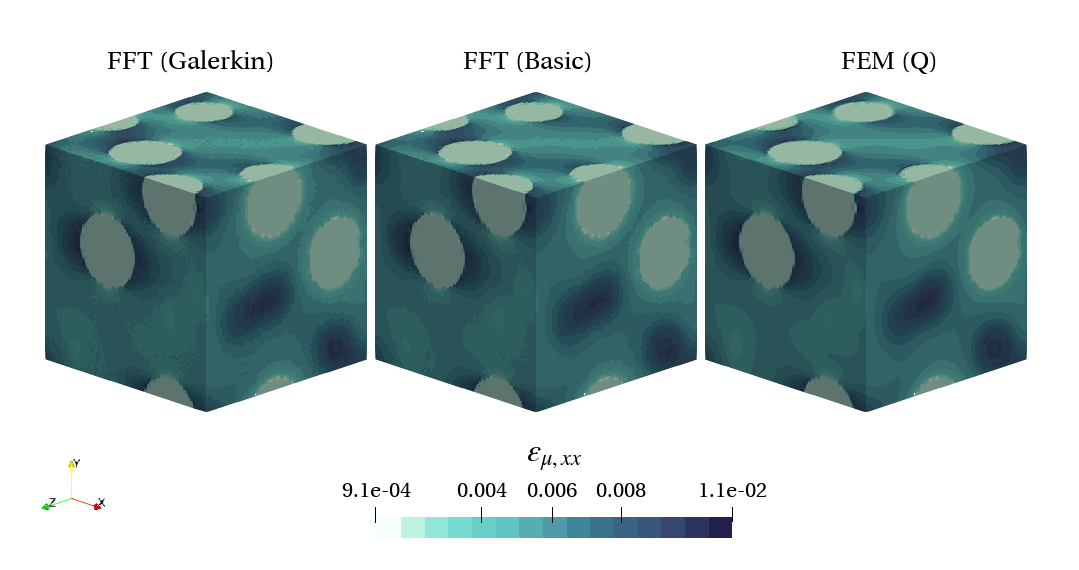
\includegraphics[width=\textwidth]{figures/linear_3D_normal_strain_11}
    \caption{}
    \label{subfig:linear_3D_normal_strain_11}
  \end{subfigure}
  \caption{Comparison between the FFT and FEM-based homogenization approaches in the
  solution of the particle-reinforced linear elastic composite equilibrium problem under normal
  strain loading conditions: \subref{subfig:linear_3D_normal_homo_stress_11_vs_n_voxels} Homogenized stress; \subref{subfig:linear_3D_normal_cpu_time_vs_n_voxels} Computational time; \subref{subfig:linear_3D_normal_strain_11} Local strain field
  (\(n_v = 70 \times 70\times 70\) discretization). Notation: linear element (L), quadratic element (Q), direct solver
  (DS) and iterative solver (IS)}
  \label{fig:linear_3D_normal}
\end{figure}

\begin{figure}[hbt] % fig:linear_3D_shear
  \centering
	\begin{subfigure}[b]{0.49\textwidth}
    \centering
    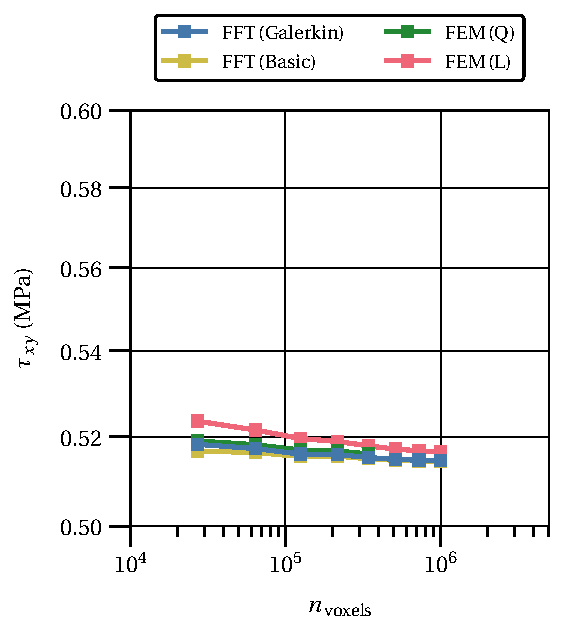
\includegraphics[width=\textwidth]{figures/linear_3D_shear_homo_stress_12_vs_n_voxels}
    \caption{}
    \label{subfig:linear_3D_shear_homo_stress_12_vs_n_voxels}
  \end{subfigure}
  \begin{subfigure}[b]{0.49\textwidth}
    \centering
    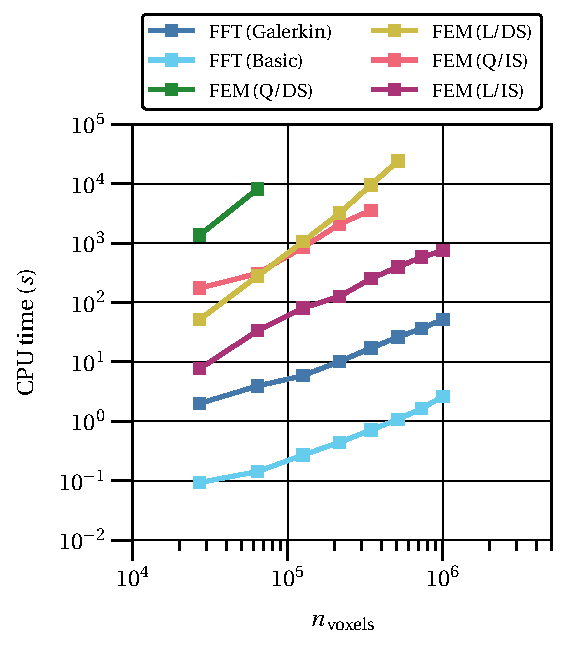
\includegraphics[width=\textwidth]{figures/linear_3D_shear_cpu_time_vs_n_voxels}
    \caption{}
    \label{subfig:linear_3D_shear_cpu_time_vs_n_voxels}
  \end{subfigure}
  \begin{subfigure}[b]{\textwidth}
    \centering
    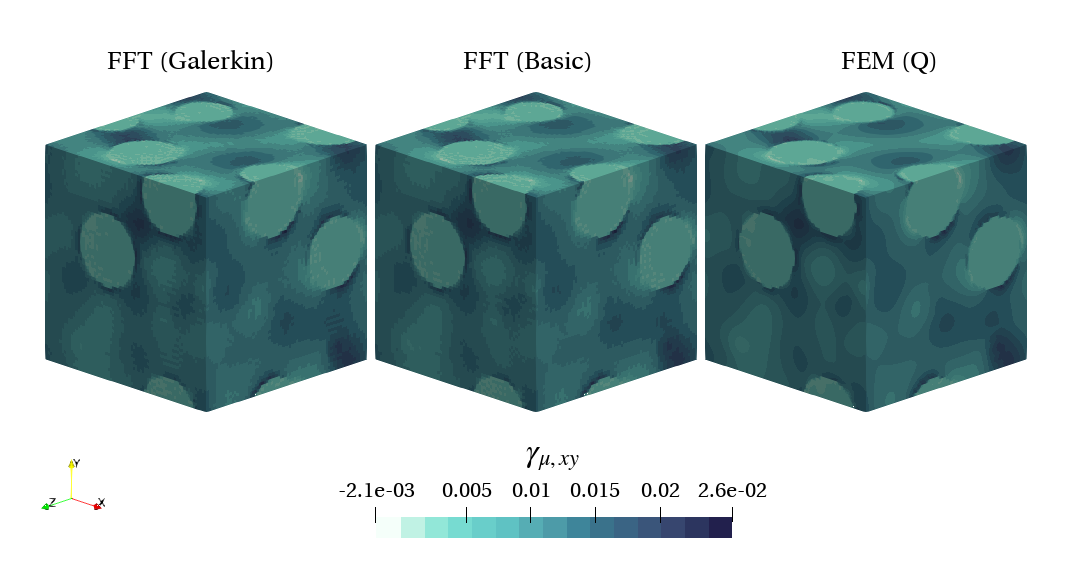
\includegraphics[width=\textwidth]{figures/linear_3D_shear_strain_12}
    \caption{}
    \label{subfig:linear_3D_shear_strain_12}
  \end{subfigure}
  \caption{Comparison between the FFT and FEM-based homogenization approaches in the
  solution of the fiber-reinforced linear elastic composite equilibrium problem under pure shear
  strain loading conditions: \subref{subfig:linear_3D_shear_homo_stress_12_vs_n_voxels} Homogenized stress; \subref{subfig:linear_3D_normal_cpu_time_vs_n_voxels} Computational time; \subref{subfig:linear_3D_normal_strain_11} Local strain field
  (\(n_v = 70 \times 70 \times 70\) discretization). Notation: linear element (L), quadratic element (Q), direct solver
  (DS) and iterative solver (IS).}
  \label{fig:linear_3D_shear}
\end{figure}

From the results present, a few conclusions and remarks are in order:
\begin{itemize}
  \item The FFT-based homogenization Galerkin scheme implementation is validated as solutions obtained (both homogenized results and local fields) are in excellent agreement with ones obtained with the FEM-based homogenization from LINKS and the FFT-based homogenization basic scheme;
  \item In the linear elastic regime, the FFT-based homogenization Galerkin scheme outperforms the FEM-based homogenization both in terms of speed and memory footprint.
  However, it must be kept in the mind that some of the Python libraries employed in the implementation of the FFT-based homogenization Galerkin scheme are parallelized and only one core was used in the LINKS simulations.
  \item In the linear elastic regime, the FFT-based homogenization basic scheme outperforms the FFT-based homogenization Galerkin scheme in terms of CPU time expended.
  Yet, consider that the implementation of the basic scheme used in the comparison \cite{} has already undergone some perfomance optimization.
  This is not the case for the Galerkin scheme.
  \item Given the solution convergence with the increasing sampling/meshing refinement, the spatial discretizations of \(n_{v}=600 \times 600\) (fiber-reinforced composite 2D RVE) and \(n_{v}=70 \times\) \(70 \times 70\) (particle-reinforced composite 3D RVE) are considered hereafter unless otherwise stated;
  \item In the following numerical studies, the reference DNS solution is obtained considering quadratic finite elements (QUAD8 and HEXA20) and the fastest solver time (MKL PARDISO in the 2D case and WSMP-SSOR in the \(3 \mathrm{D}\) case) unless otherwise stated.
\end{itemize}

\FloatBarrier

\paragraph{Extreme stiffness ratios between phases}

The following set of results is presented to better comprehend the limitations of the FFT-based methods regarding the stiffness ratio between the phases, widely reported in the literature \cite{}.
As previously, FEM solutions are used as a standard.

Both phases are assumed linear elastic having the same Poisson's ratio, \(\nu=0.3\).
The Young modulus of the matrix is fixed at \(E_1=\SI{100}{\mega\pascal}\) and the ratio between the stiffness of the particles and the matrix, \(K=E_1/E_2\), is made to vary from \num{e-6} to \num{e4} in increments of \(\times \sqrt{10}\).
Periodic boundary conditions are adopted and the following macroscale strain loading case is considered
\begin{equation}
\text { uniaxial: } \bm{\varepsilon}=\left[\begin{array}{lll}
5 & 0 & 0 \\
0 & 0 & 0 \\
0 & 0 & 0
\end{array}\right] \times 10^{-3},
\end{equation}
being enforced in a single load increment.
Note that in the 2D plane strain case, only the inplane \(O_{x y}\) macroscale strain components are enforced.

The numerical results of the fiber-reinforced linear elastic composite equilibrium problem are shown in Figures~\ref{fig:linear_2D_normal_stiff_contrast} for the uniaxial loading case.
There is an excellent agreement between the FFT and FEM-based homogenization solutions concerning the homogenized response as attested by Figure~\ref{subfig:linear_2D_normal_stress_avg_vs_stiff_ratio}.
In terms of computational performance, Figure~\ref{subfig:linear_2D_normal_stress_avg_cpu_time_vs_n_voxels} shows that the FFT-based homogenization Galerkin scheme outperforms the FEM-based homogenization with speedups from around 20 at low stiffness contrast to around 2 at the hightest stiffness contrasts, both high and low, relative to the direct solver with linear finite elements.
As before, the caveat regarding the parallelization of the Python libraries still applies.
When compared with the FFT-based homogenization basic scheme, the CPU time expended differs from one to two orders of magnitude across the stiffness ranges considered, with the Galerkin scheme being slower.
However, the basic scheme is unable to reach the preset tolerance \((\num{e-6})\) for stiffness ratios beyond the range \([\num{e-3},\num{e3}]\).

Concerning the local field, an excellent agreement can be observed at both high \((K=E_1/E_2=\num{e4})\) and low \((K=E_1/E_2=\num{e-4})\) stiffness ratios in the matrix phase, as can be seen in Figures~\ref{fig:linear_2D_stiff_contrast_normal_strain_11} and \ref{fig:linear_2D_stiff_contrast_normal_stress_11}.
There is also good agreement regarding the local field in the particle phase for the strain field at the low stiffness ratio and the stress field at the high stiffness ratio.
On the other hand, the strain field at the low stiffness ratio and the strain field at the high stiffness ratio exihibt strong oscillations in the particle phase.
This phenomenon is often denominated by "ringing" and is widely reported in the literature as being a consequence of very high or low stiffness ratios.
Figure~\ref{} provides a more detailed representation of the variation of the strain field \(\varepsilon_{\mu,xx}\) inside the particle pahse at a stiffness ratio equal to \num{e-4}.


\begin{figure}[hbt]
  \centering
  	\begin{subfigure}[b]{0.49\textwidth}
      \centering
      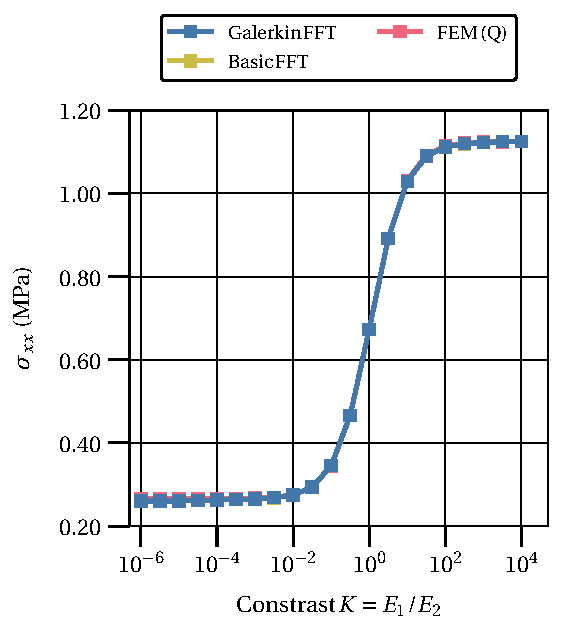
\includegraphics[width=\textwidth]{figures/linear_2D_normal_stress_avg_vs_stiff_ratio}
      \caption{}
      \label{subfig:linear_2D_normal_stress_avg_vs_stiff_ratio}
    \end{subfigure}
    \begin{subfigure}[b]{0.49\textwidth}
      \centering
      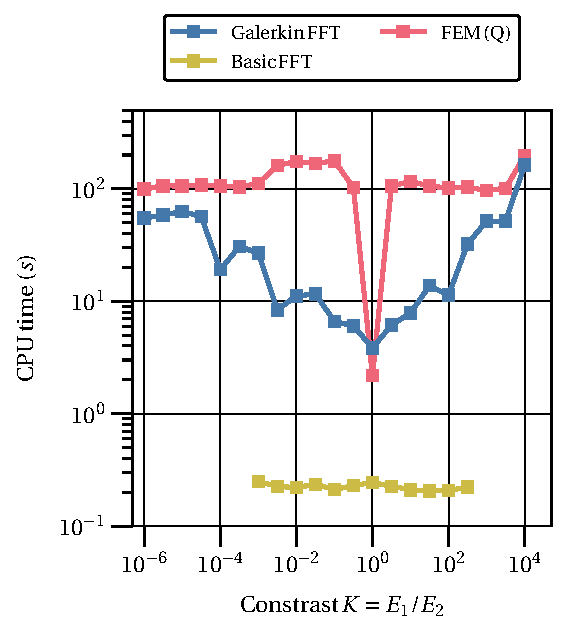
\includegraphics[width=\textwidth]{figures/linear_2D_normal_stress_avg_cpu_time_vs_n_voxels}
      \caption{}
      \label{subfig:linear_2D_normal_stress_avg_cpu_time_vs_n_voxels}
    \end{subfigure}
  \caption{Comparison between the FFT and FEM-based homogenization approaches in the solution
  of the fiber-reinforced linear elastic composite equilibrium problem under normal strain
  loading conditions: \subref{subfig:linear_2D_normal_stress_avg_vs_stiff_ratio} Homogenized
  stress; \subref{subfig:linear_2D_normal_stress_avg_cpu_time_vs_n_voxels} Computational time;
  Notation: linear element (L), quadratic element (Q).}
\label{fig:linear_2D_normal_stiff_contrast}
\end{figure}

\begin{figure}[hbt]
  \centering
	\begin{subfigure}[b]{\textwidth}
    \centering
    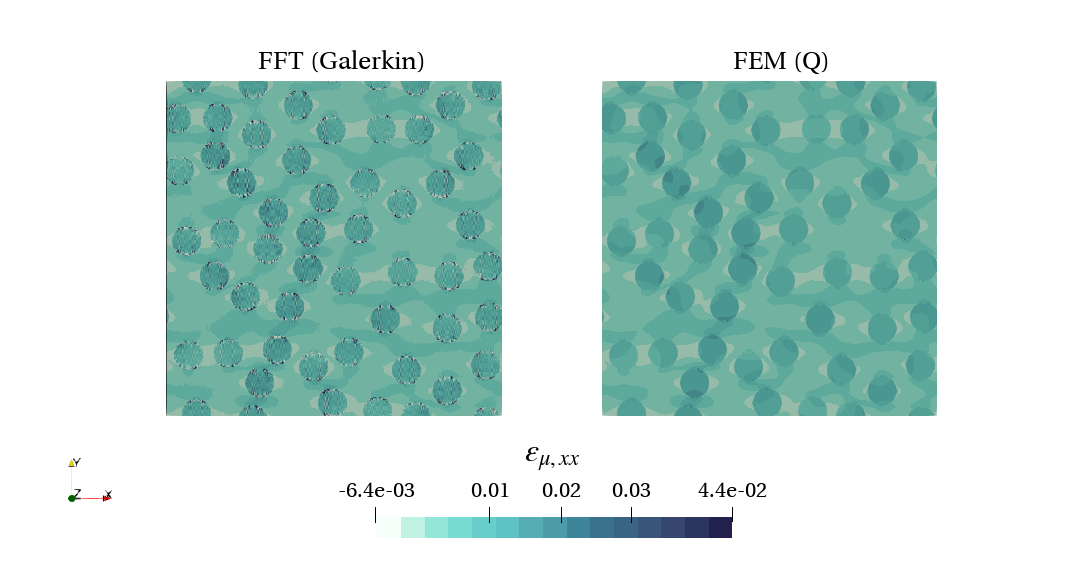
\includegraphics[width=\textwidth]{figures/linear_2D_ratio_-4_normal_strain_11}
    \caption{}
    \label{subfig:linear_2D_ratio_-4_normal_strain_11}
  \end{subfigure}
  \begin{subfigure}[b]{\textwidth}
    \centering
    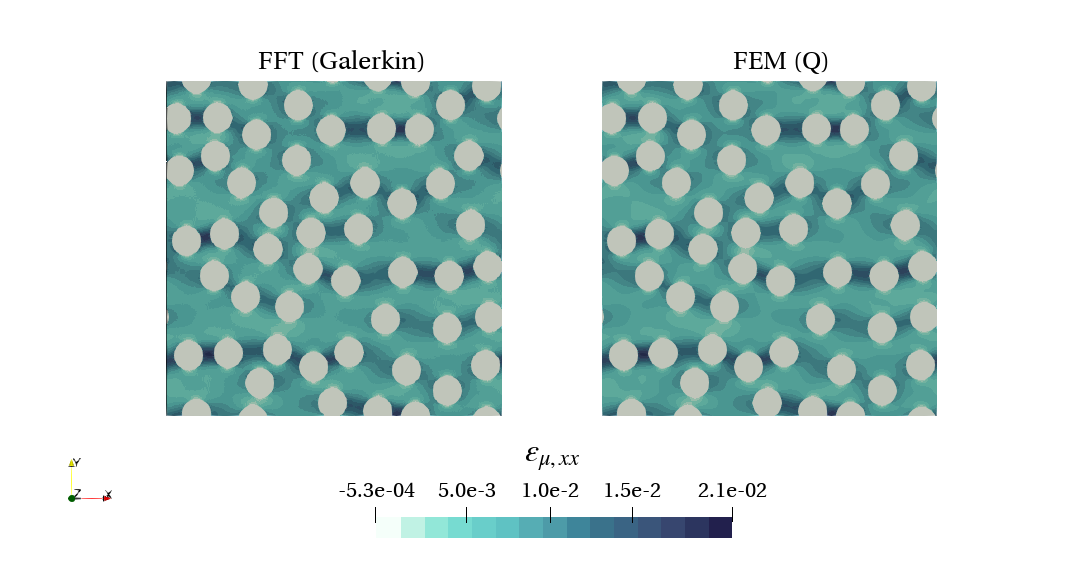
\includegraphics[width=\textwidth]{figures/linear_2D_ratio_4_normal_strain_11}
    \caption{}
    \label{subfig:linear_2D_ratio_4_normal_strain_11}
  \end{subfigure}
  \caption{Comparison between the local strain field \(\varepsilon_{\mu,xx}\) obtained using
  FFT and FEM-based homogenization approaches in the solution of the fiber-reinforced
  linear elastic composite equilibrium problem under normal strain loading conditions:
  \subref{subfig:linear_2D_ratio_-4_normal_strain_11} Stiffness ratio \(K=E_1/E_2=\num{e-4}\);
  \subref{subfig:linear_2D_ratio_4_normal_strain_11} Stiffness ratio \(K=E_1/E_2=\num{e1.5}\);
  Notation: quadratic element (Q).}
\label{fig:linear_2D_stiff_contrast_normal_strain_11}
\end{figure}

\begin{figure}[hbt]
  \centering
	\begin{subfigure}[b]{\textwidth}
    \centering
    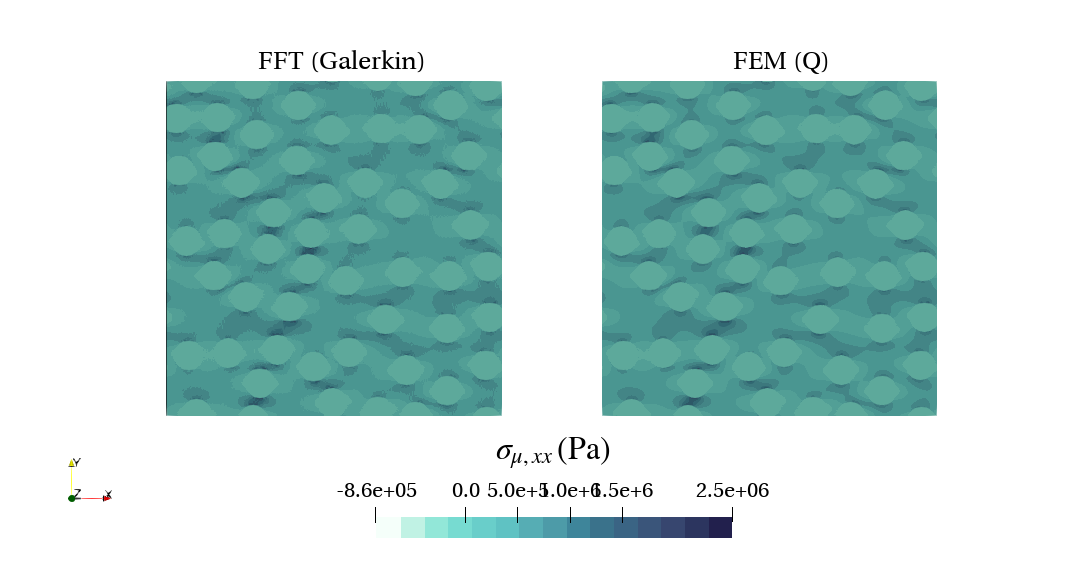
\includegraphics[width=\textwidth]{figures/linear_2D_ratio_-4_normal_stress_11}
    \caption{}
    \label{subfig:linear_2D_ratio_4_normal_stress_11}
  \end{subfigure}
  \begin{subfigure}[b]{\textwidth}
    \centering
    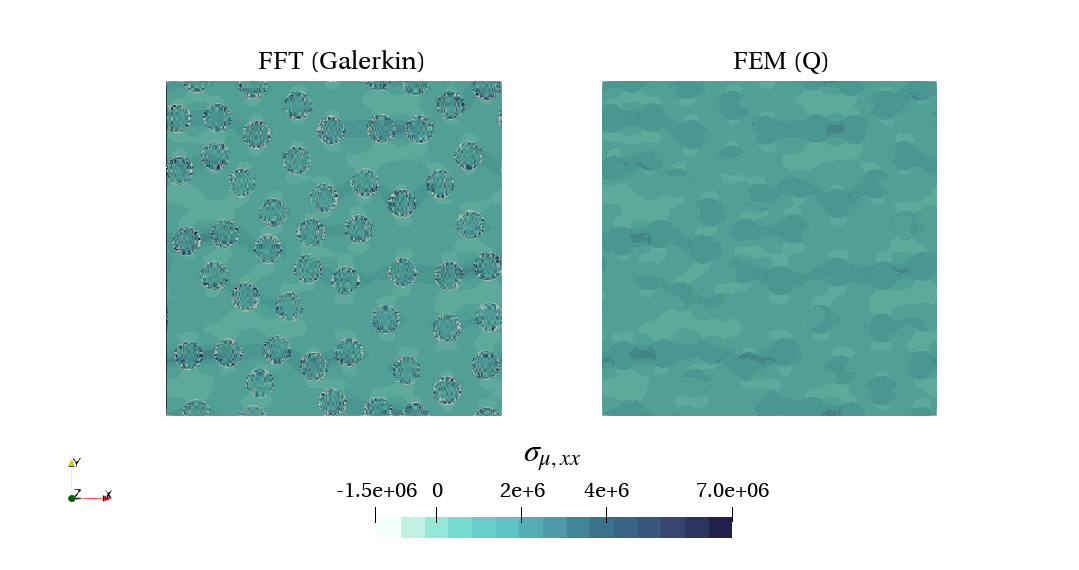
\includegraphics[width=\textwidth]{figures/linear_2D_ratio_4_normal_stress_11}
    \caption{}
    \label{subfig:linear_2D_ratio_-4_normal_stress_11}
  \end{subfigure}
  \caption{Comparison between the local stress field \(\sigma_{\mu,xx}\) obtained using
  FFT and FEM-based homogenization approaches in the solution of the fiber-reinforced
  linear elastic composite equilibrium problem under normal strain loading conditions:
  \subref{subfig:linear_2D_ratio_-4_normal_stress_11} Stiffness ratio \(K=E_1/E_2=\num{e-4}\);
  \subref{subfig:linear_2D_ratio_4_normal_stress_11} Stiffness ratio \(K=E_1/E_2=\num{e1.5}\);
  Notation: quadratic element (Q).}
\label{fig:linear_2D_stiff_contrast_normal_stress_11}
\end{figure}

\begin{figure}[hbt]
  \centering
  	\begin{subfigure}[b]{0.49\textwidth}
      \centering
      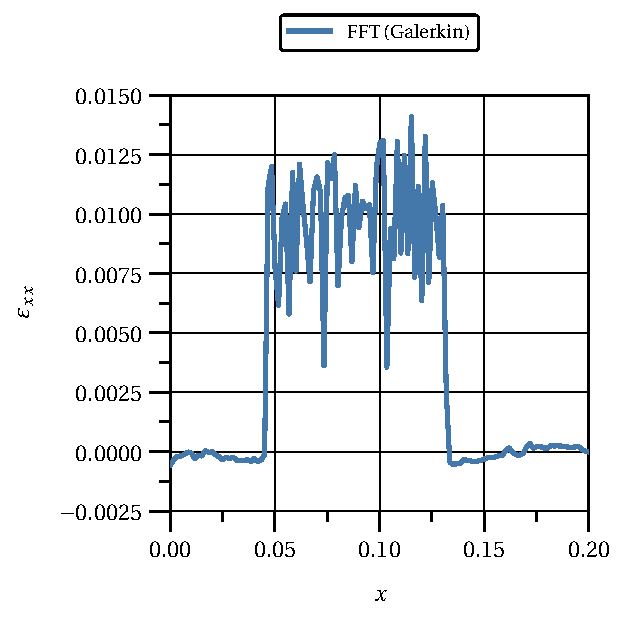
\includegraphics[width=\textwidth]{figures/linear_2D_ratio_-4_normal_strain_11_particle_1}
      \caption{}
      \label{subfig:linear_2D_ratio_-4_normal_strain_11_particle_1}
    \end{subfigure}
    \begin{subfigure}[b]{0.49\textwidth}
      \centering
      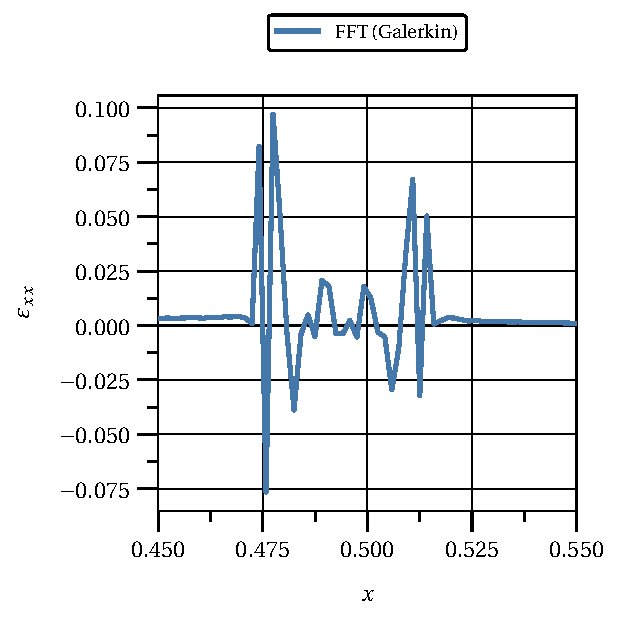
\includegraphics[width=\textwidth]{figures/linear_2D_ratio_-4_normal_strain_11_particle_2}
      \caption{}
      \label{subfig:linear_2D_ratio_-4_normal_strain_11_particle_2}
    \end{subfigure}
  \caption{Comparison between the FFT and FEM-based homogenization approaches in the solution
  of the fiber-reinforced linear elastic composite equilibrium problem under pure shear strain
  loading conditions: \subref{subfig:linear_2D_normal_stress_avg_vs_stiff_ratio} Homogenized
  stress; \subref{subfig:linear_2D_normal_stress_avg_cpu_time_vs_n_voxels} Computational time;
  Notation: linear element (L), quadratic element (Q).}
\label{fig:linear_2D_ratio_-4_normal_strain_11_particles}
\end{figure}

The numerical results of the particle-reinforced linear elastic composite equilibrium problem are shown in Figures~\ref{fig:linear_3D_normal_stiff_contrast} for the uniaxial loading case.
There is an excellent agreement between the FFT-based homogenization Galerkin scheme and the FEM-based homogenization solutions concerning the homogenized response as attested by Figure~\ref{subfig:linear_3D_normal_stress_avg_vs_stiff_ratio}.
Same cannot be said for the FFT-based homogenization Galerkin scheme as the stiffness ratio becomes more extreme.
In terms of computational performance, Figure~\ref{subfig:linear_3D_normal_stress_avg_cpu_time_vs_n_voxels} shows that the FFT-based homogenization Galerkin scheme outperforms the FEM-based homogenization with speedups from around 100 at minor stiffness contrast to around 3 at the lowest stiffness contrast, relative to the direct solver with linear finite elements.
As before, the caveat regarding the parallelization of the Python libraries still applies.
When compared with the FFT-based homogenization basic scheme, the CPU time expended differs from one to two orders of magnitude across the stiffness ranges considered, with the Galerkin scheme being slower.
It must be added that for higher stiffness ratios the WSMP-SSOR solver was not able to converge.

Concerning the local field, an excellent agreement can be observed at both high \((K=E_1/E_2=10^{1.5})\) and low \((K=E_1/E_2=\num{e-4})\) stiffness ratios in the matrix phase, as can be seen in Figures~\ref{fig:linear_3D_stiff_contrast_normal_strain_11} and \ref{fig:linear_3D_stiff_contrast_normal_stress_11}.
There is also good agreement regarding the local field in the particle phase for the strain field at the low stiffness ratio and the stress field at the high stiffness ratio.
On the other hand, the strain field at the low stiffness ratio and the strain field at the high stiffness ratio exihibt strong oscillations in the particle phase.
This mirrors the previous results concerning two dimensional microstructures.

\begin{figure}[hbt]
  \centering
  	\begin{subfigure}[b]{0.49\textwidth}
      \centering
      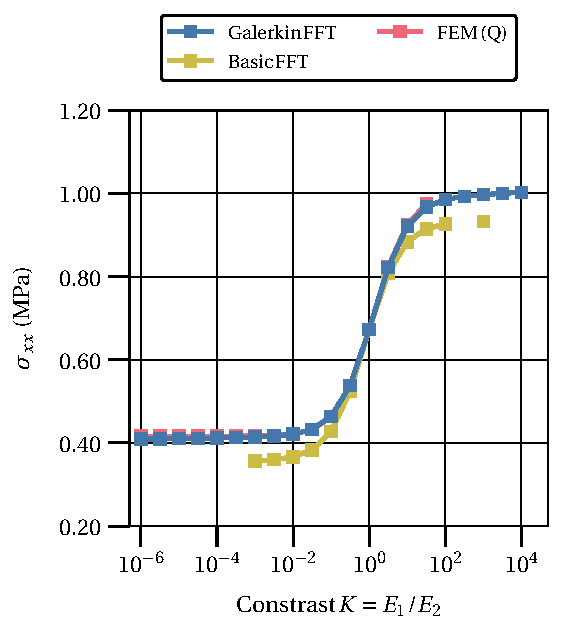
\includegraphics[width=\textwidth]{figures/linear_3D_normal_stress_avg_vs_stiff_ratio}
      \caption{}
      \label{subfig:linear_3D_normal_stress_avg_vs_stiff_ratio}
    \end{subfigure}
    \begin{subfigure}[b]{0.49\textwidth}
      \centering
      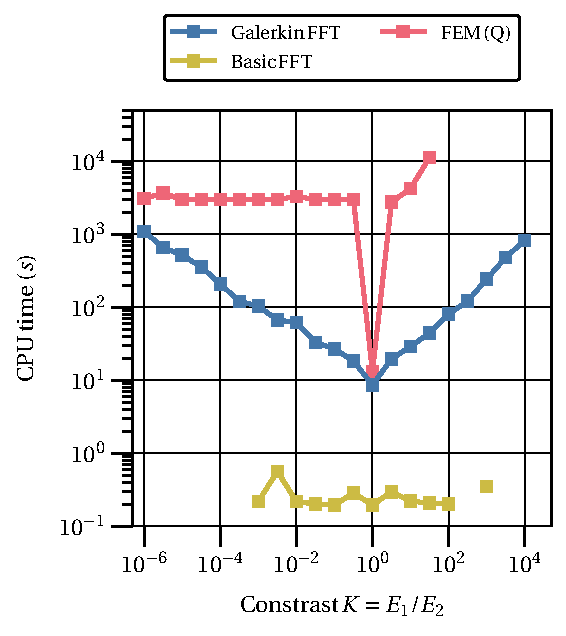
\includegraphics[width=\textwidth]{figures/linear_3D_normal_stress_avg_cpu_time_vs_n_voxels}
      \caption{}
      \label{subfig:linear_3D_normal_stress_avg_cpu_time_vs_n_voxels}
    \end{subfigure}
  \caption{Comparison between the FFT and FEM-based homogenization approaches in the solution
  of the particle-reinforced linear elastic composite equilibrium problem under normal strain
  loading conditions: \subref{subfig:linear_3D_normal_stress_avg_vs_stiff_ratio} Homogenized
  stress; \subref{subfig:linear_3D_normal_stress_avg_cpu_time_vs_n_voxels} Computational time;
  Notation: linear element (L), quadratic element (Q).}
\label{fig:linear_3D_normal_stiff_contrast}
\end{figure}

\begin{figure}[hbt]
  \centering
	\begin{subfigure}[b]{\textwidth}
    \centering
    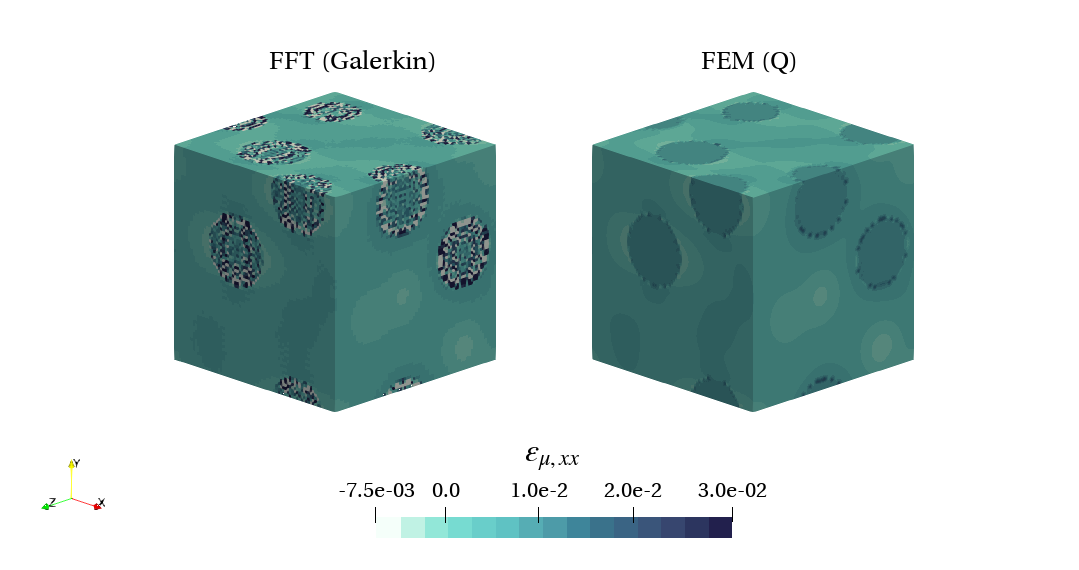
\includegraphics[width=\textwidth]{figures/linear_3D_ratio_-4_normal_strain_11}
    \caption{}
    \label{subfig:linear_3D_ratio_-4_normal_strain_11}
  \end{subfigure}
  \begin{subfigure}[b]{\textwidth}
    \centering
    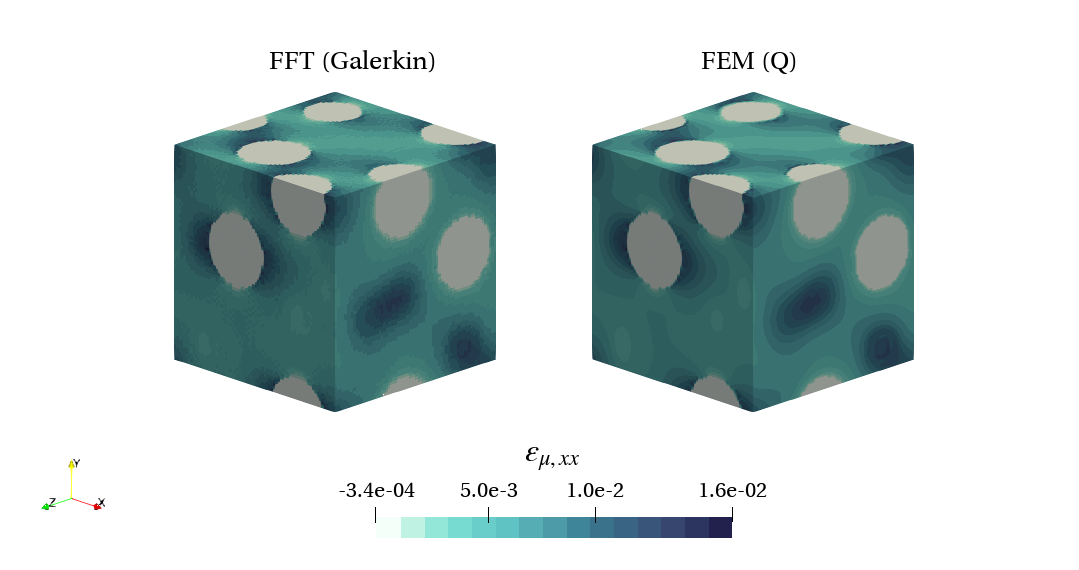
\includegraphics[width=\textwidth]{figures/linear_3D_ratio_1_5_normal_strain_11}
    \caption{}
    \label{subfig:linear_3D_ratio_1_5_normal_strain_11}
  \end{subfigure}
  \caption{Comparison between the local strain field \(\varepsilon_{\mu,xx}\) obtained using
  FFT and FEM-based homogenization approaches in the solution of the particle-reinforced
  linear elastic composite equilibrium problem under normal strain loading conditions:
  \subref{subfig:linear_3D_ratio_-4_normal_strain_11} Stiffness ratio \(K=E_1/E_2=\num{e-4}\);
  \subref{subfig:linear_3D_ratio_1_5_normal_strain_11} Stiffness ratio \(K=E_1/E_2=\num{e1.5}\);
  Notation: quadratic element (Q).}
\label{fig:linear_3D_stiff_contrast_normal_strain_11}
\end{figure}

\begin{figure}[hbt]
  \centering
	\begin{subfigure}[b]{\textwidth}
    \centering
    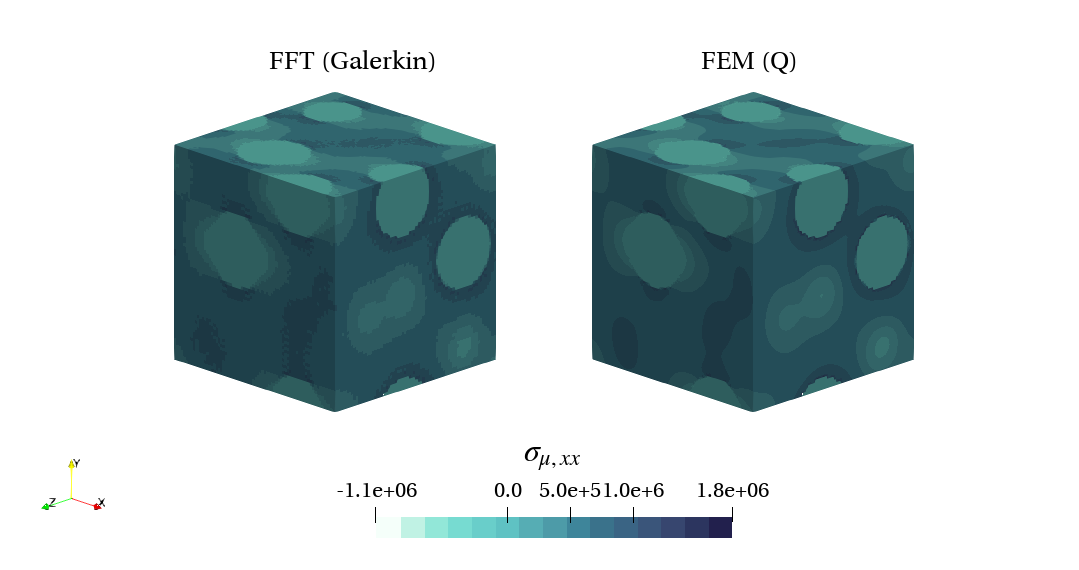
\includegraphics[width=\textwidth]{figures/linear_3D_ratio_-4_normal_stress_11}
    \caption{}
    \label{subfig:linear_3D_ratio_1_5_normal_stress_11}
  \end{subfigure}
  \begin{subfigure}[b]{\textwidth}
    \centering
    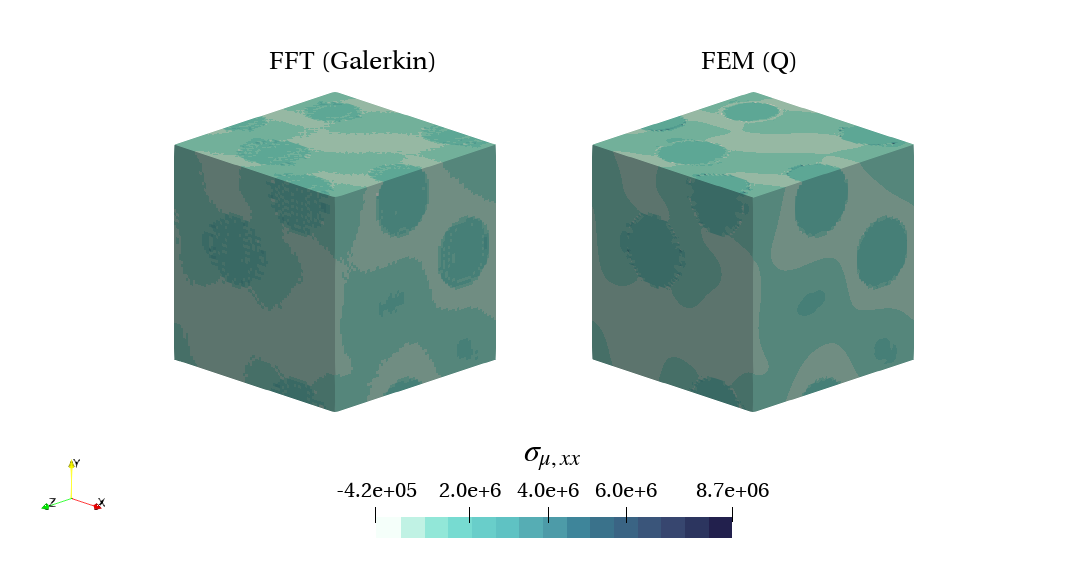
\includegraphics[width=\textwidth]{figures/linear_3D_ratio_1_5_normal_stress_11}
    \caption{}
    \label{subfig:linear_3D_ratio_-4_normal_stress_11}
  \end{subfigure}
  \caption{Comparison between the local stress field \(\sigma_{\mu,xx}\) obtained using
  FFT and FEM-based homogenization approaches in the solution of the particle-reinforced
  linear elastic composite equilibrium problem under normal strain loading conditions:
  \subref{subfig:linear_3D_ratio_-4_normal_stress_11} Stiffness ratio \(K=E_1/E_2=\num{e-4}\);
  \subref{subfig:linear_3D_ratio_1_5_normal_stress_11} Stiffness ratio \(K=E_1/E_2=\num{e1.5}\);
  Notation: quadratic element (Q).}
\label{fig:linear_3D_stiff_contrast_normal_stress_11}
\end{figure}


\FloatBarrier

\subsection{Large strain}

\paragraph{Accuracy validation}

\subparagraph{Hencky}

\begin{figure}[hbt]
  \centering
	\begin{subfigure}[b]{0.49\textwidth}
    \centering
    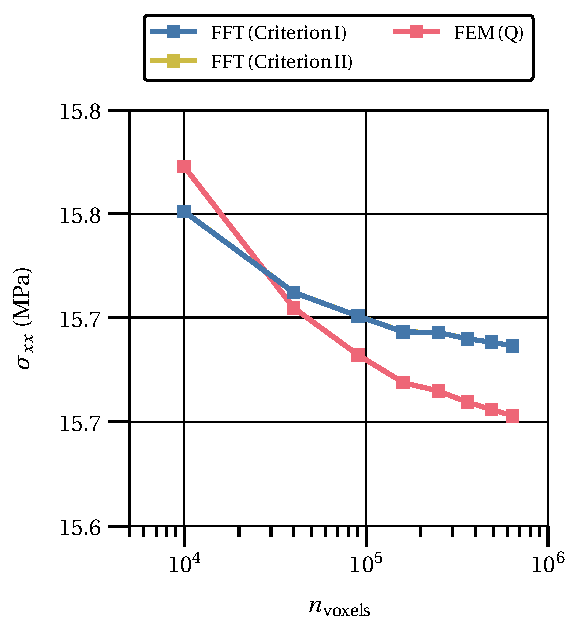
\includegraphics[width=\textwidth]{figures/hencky_2D_normal_homo_stress_11_vs_n_voxels}
    \caption{}
    \label{subfig:hencky_2D_normal_homo_stress_11_vs_n_voxels}
  \end{subfigure}
  \begin{subfigure}[b]{0.49\textwidth}
    \centering
    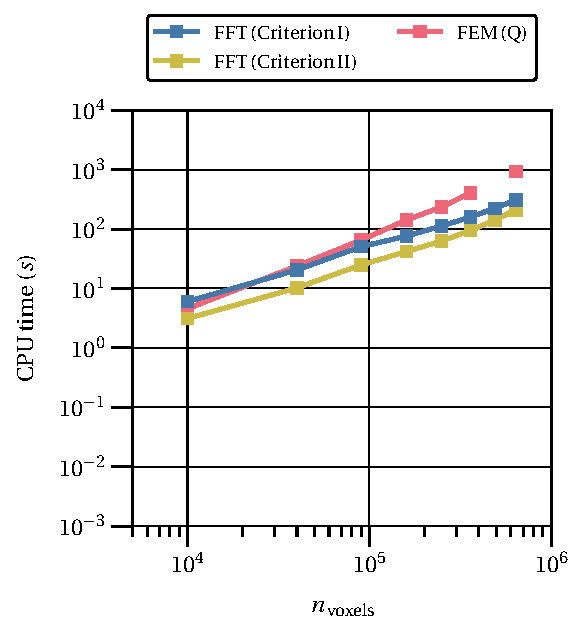
\includegraphics[width=\textwidth]{figures/hencky_2D_normal_cpu_time_vs_n_voxels}
    \caption{}
    \label{subfig:hencky_2D_normal_cpu_time_vs_n_voxels}
  \end{subfigure}
  \begin{subfigure}[b]{\textwidth}
    \centering
    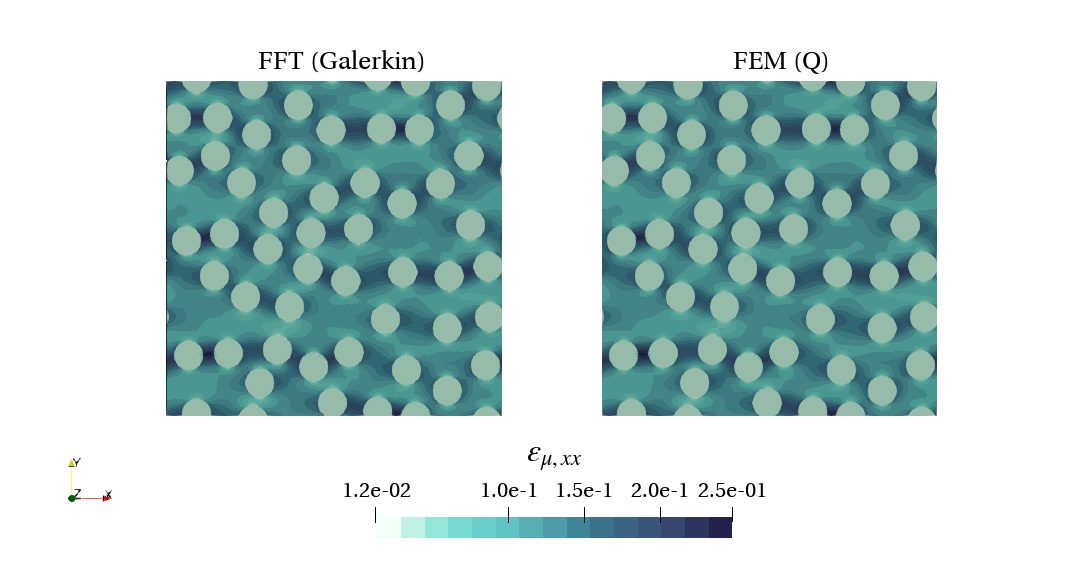
\includegraphics[width=\textwidth]{figures/hencky_2D_normal_strain_11}
    \caption{}
    \label{subfig:hencky_2D_normal_strain_11}
  \end{subfigure}
  \caption{Comparison between the Criterion I and II for FFT-based homogenization approaches, Galerkin and Basic, in the
  solution of the particle-reinforced hencky elastic composite equilibrium problem under uniaxial
  strain loading conditions: \subref{subfig:hencky_2D_shear_comparison_crit_homo_stress_12_vs_n_voxels} Homogenized stress; \subref{subfig:hencky_2D_shear_comparison_crit_cpu_time_vs_n_voxels} Computational time.}
\label{fig:hencky_2D_normal}
\end{figure}

\begin{figure}[hbt]
  \centering
	\begin{subfigure}[b]{0.49\textwidth}
    \centering
    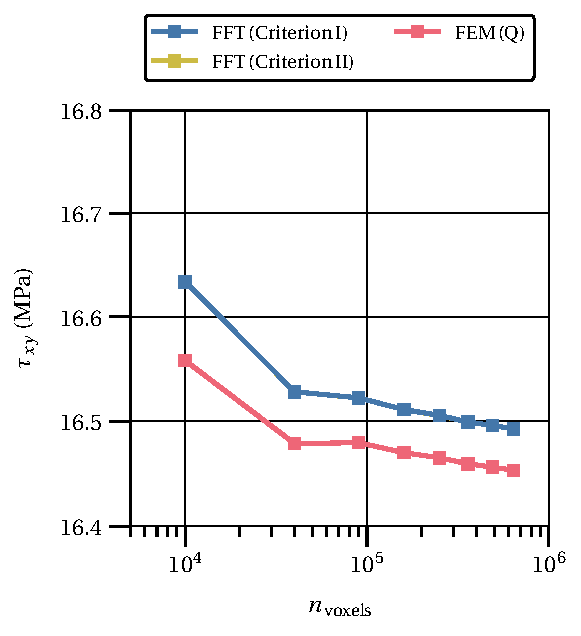
\includegraphics[width=\textwidth]{figures/hencky_2D_shear_homo_stress_12_vs_n_voxels}
    \caption{}
    \label{subfig:hencky_2D_shear_homo_stress_12_vs_n_voxels}
  \end{subfigure}
  \begin{subfigure}[b]{0.49\textwidth}
    \centering
    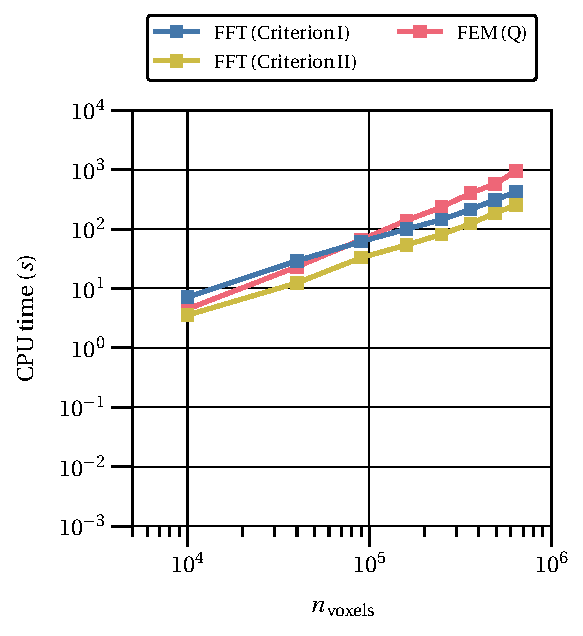
\includegraphics[width=\textwidth]{figures/hencky_2D_shear_cpu_time_vs_n_voxels}
    \caption{}
    \label{subfig:hencky_2D_shear_cpu_time_vs_n_voxels}
  \end{subfigure}
  \begin{subfigure}[b]{\textwidth}
    \centering
    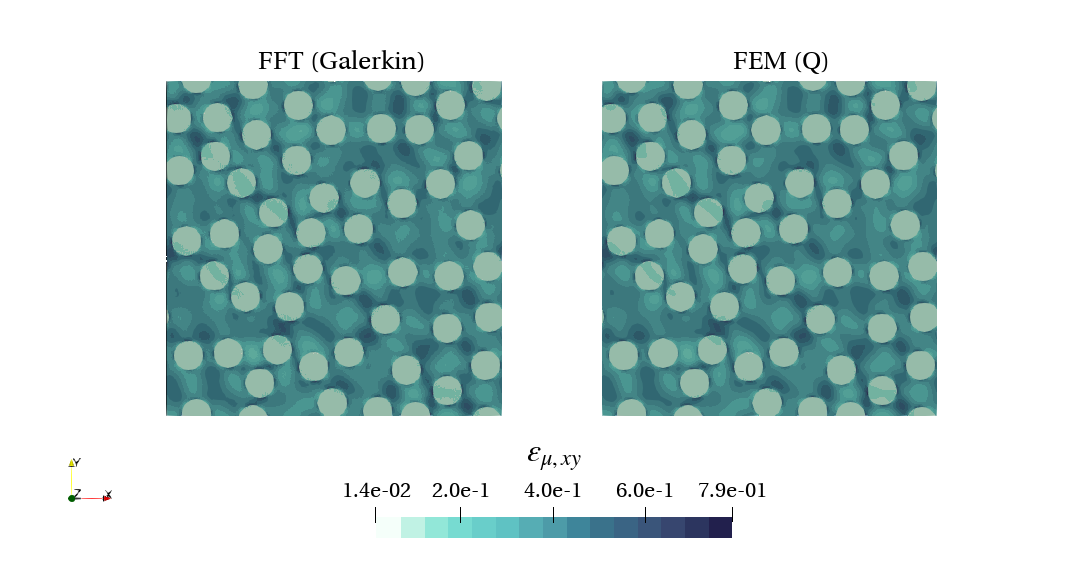
\includegraphics[width=\textwidth]{figures/hencky_2D_shear_strain_12}
    \caption{}
    \label{subfig:hencky_2D_shear_strain_12}
  \end{subfigure}
  \caption{f}
\label{fig:hencky_2D_shear}
\end{figure}

\begin{figure}[hbt] % incomplete
\label{fig:hencky_mat_res_2D_normal}
\end{figure}

\begin{figure}[hbt] % incomplete
\label{fig:hencky_mat_res_2D_shear}
\end{figure}

\begin{figure}[hbt] % incomplete
\label{fig:hencky_mat_res_3D_normal}
\end{figure}

\begin{figure}[hbt] % incomplete
\label{fig:hencky_mat_res_3D_shear}
\end{figure}

\FloatBarrier

\subparagraph{Saint Venant-Kirchhoff model}

\begin{figure}[hbt]
  \centering
	\begin{subfigure}[b]{0.49\textwidth}
    \centering
    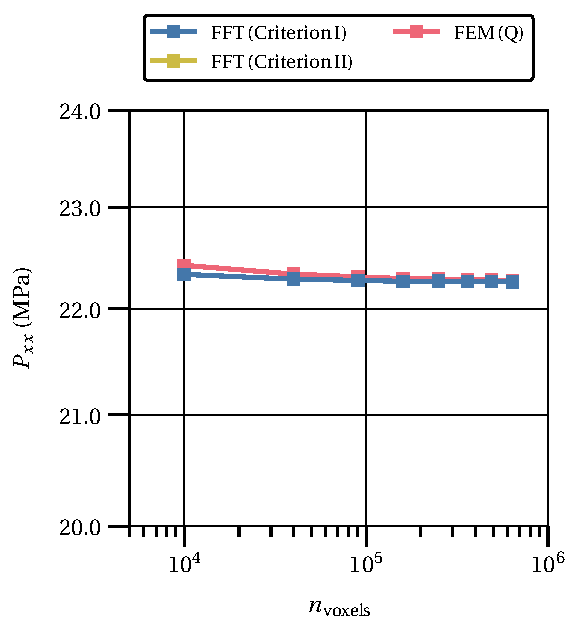
\includegraphics[width=\textwidth]{figures/svk_2D_normal_homo_stress_11_vs_n_voxels}
    \caption{}
    \label{subfig:svk_2D_normal_homo_stress_11_vs_n_voxels}
  \end{subfigure}
  \begin{subfigure}[b]{0.49\textwidth}
    \centering
    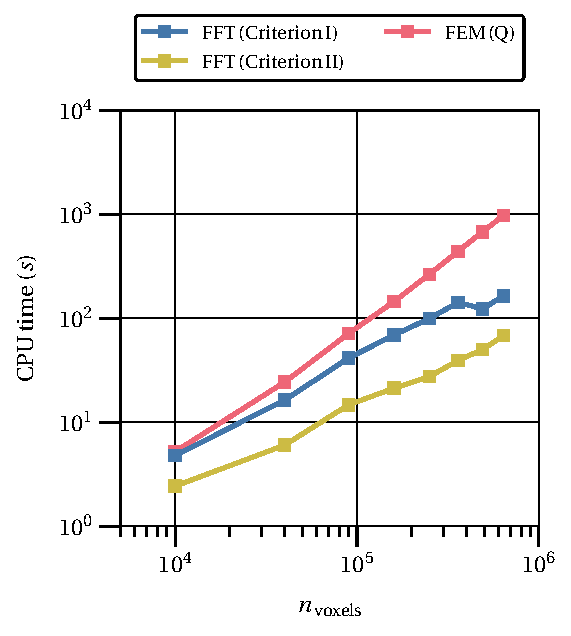
\includegraphics[width=\textwidth]{figures/svk_2D_normal_cpu_time_vs_n_voxels}
    \caption{}
    \label{subfig:svk_2D_normal_cpu_time_vs_n_voxels}
  \end{subfigure}
  \begin{subfigure}[b]{\textwidth}
    \centering
    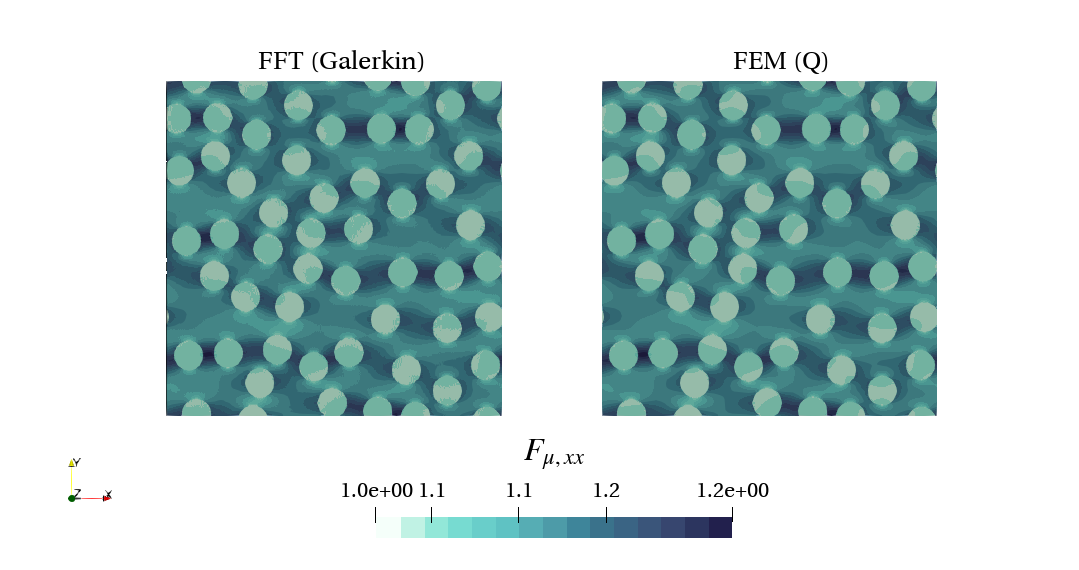
\includegraphics[width=\textwidth]{figures/svk_2D_normal_strain_11}
    \caption{}
    \label{subfig:svk_2D_normal_strain_11}
  \end{subfigure}
  \caption{Comparison between the Criterion I and II for FFT-based homogenization
  approaches, Galerkin and Basic, in the solution of the particle-reinforced svk elastic
  composite equilibrium problem under uniaxial strain loading conditions:
  \subref{subfig:svk_2D_normal_comparison_crit_homo_stress_11_vs_n_voxels} Homogenized
  stress; \subref{subfig:svk_2D_normal_comparison_crit_cpu_time_vs_n_voxels} Computational
  time.}
\label{fig:svk_2D_normal}
\end{figure}

\FloatBarrier

\paragraph{Extreme stiffness ratios between phases}

\subparagraph{Hencky}

\subparagraph{Saint Venant-Kirchhoff model}

\begin{figure}[hbt]
  \centering
	\begin{subfigure}[b]{0.49\textwidth}
    \centering
    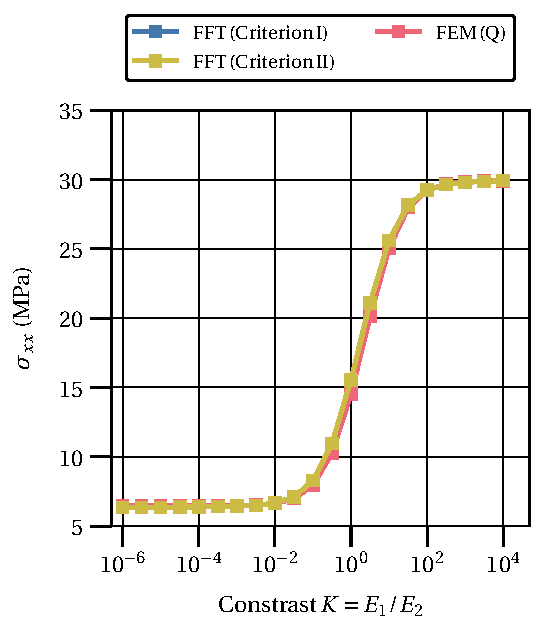
\includegraphics[width=\textwidth]{figures/svk_2D_normal_stress_avg_vs_stiff_ratio}
    \caption{}
    \label{subfig:svk_2D_normal_stress_avg_vs_stiff_ratio}
  \end{subfigure}
  \begin{subfigure}[b]{0.49\textwidth}
    \centering
    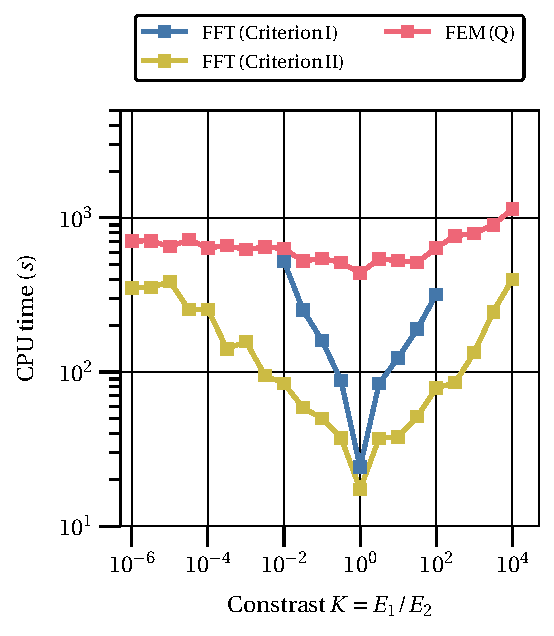
\includegraphics[width=\textwidth]{figures/svk_2D_normal_stress_avg_cpu_time_vs_n_voxels}
    \caption{}
    \label{subfig:svk_2D_normal_stress_avg_cpu_time_vs_n_voxels}
  \end{subfigure}
  \caption{Comparison between the Criterion I and II for FFT-based homogenization approaches, Galerkin and Basic, in the
  solution of the particle-reinforced svk elastic composite equilibrium problem under uniaxial
  strain loading conditions: \subref{subfig:svk_3D_normal_comparison_crit_homo_stress_11_vs_n_voxels} Homogenized stress; \subref{subfig:svk_3D_normal_comparison_crit_cpu_time_vs_n_voxels} Computational time.}
\label{fig:svk_2D_normal_stiff_contrast}
\end{figure}

\begin{figure}[hbt]
  \centering
	\begin{subfigure}[b]{\textwidth}
    \centering
    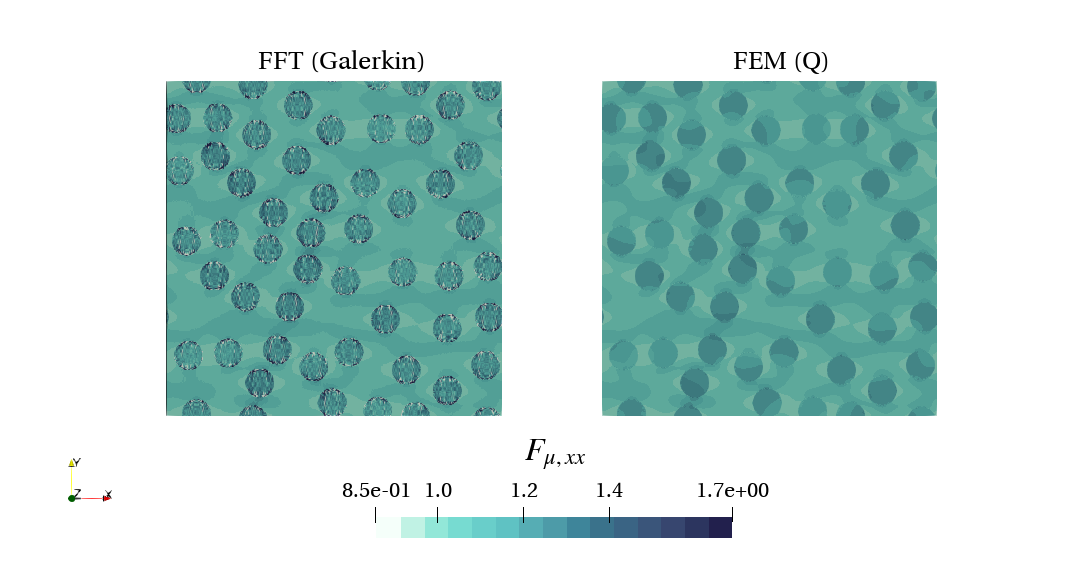
\includegraphics[width=\textwidth]{figures/svk_2D_ratio_-4_normal_strain_11}
    \caption{}
    \label{subfig:svk_2D_ratio_4_normal_strain_11}
  \end{subfigure}
  \begin{subfigure}[b]{\textwidth}
    \centering
    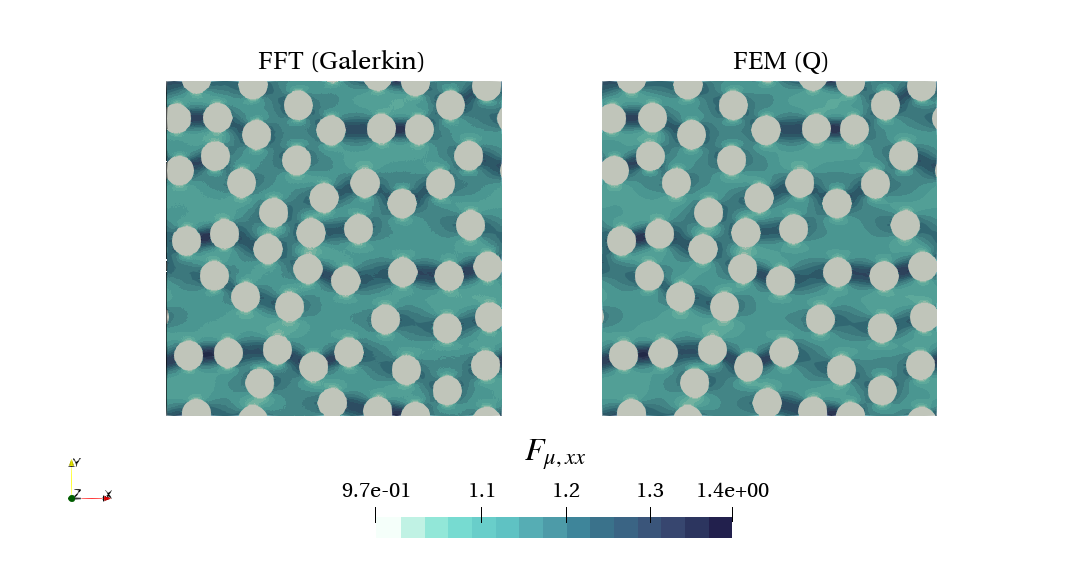
\includegraphics[width=\textwidth]{figures/svk_2D_ratio_4_normal_strain_11}
    \caption{}
    \label{subfig:svk_2D_ratio_-4_normal_strain_11}
  \end{subfigure}
  \caption{Comparison between the Criterion I and II for FFT-based homogenization approaches, Galerkin and Basic, in the
  solution of the particle-reinforced svk elastic composite equilibrium problem under uniaxial
  strain loading conditions: \subref{subfig:svk_3D_normal_comparison_crit_homo_stress_11_vs_n_voxels} Homogenized stress; \subref{subfig:svk_3D_normal_comparison_crit_cpu_time_vs_n_voxels} Computational time.}
\label{fig:svk_2D_stiff_contrast_normal_strain_11}
\end{figure}

\FloatBarrier

\chapter{Numerical Results - Elastoplasticity} \label{chapter:numerical_results_elastoplasticity}

In the following chapter, results pertaining to elastoplasticity are presented.
The validation of the FFT-based Galerkin formulation is performed on elastoplastic materials at
small strains and large strains.
The constitutive model considered is the von Mises material model.

As in the previous chapter, all the numerical results shown in this chapter are obtained
in the same machine with the specifications provided in Table~\ref{tab:specifications}.
Contrary to the previous chapter, all the available cores in the machine are used in each simulation.

\section{Material characterization}

The microstructures and linear elastic properties considered in the following can be found in Section~\ref{sec:microstructures}.
The isotropic piecewise linear strain hardening law is presented in Figure~\ref{fig:von_mises_res_mat_small_strain_2D_normal_hardening_curve}.
The yield stress, \(\sigma_y\), is given as a function of the accumulated plastic strain, \(\bar{\varepsilon}_p\) by
\begin{equation}
\label{von_mises_hardening_curve}
  \sigma_y = \begin{cases}
    0.5 + 5\bar{\varepsilon}_p,\quad 0 \leq \bar{\epsilon}_p \leq 0.04\\
    0.7 + 2(\bar{\varepsilon}_p-0.04),\quad \bar{\epsilon}_p \geq 0.04\\
  \end{cases},\quad\si{\mega\pascal}.
\end{equation}

\begin{figure}[hbtp]
  \centering
  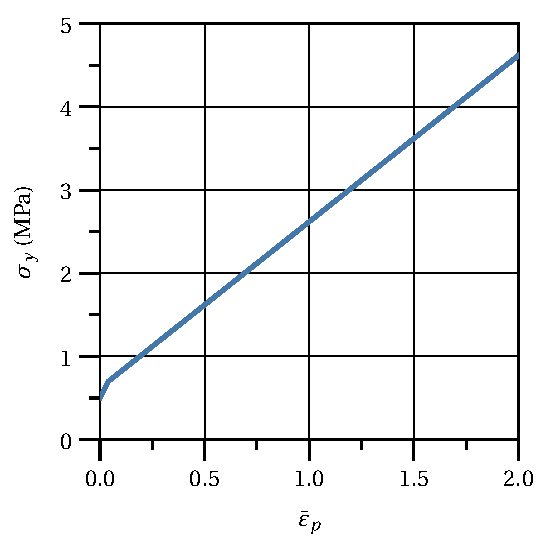
\includegraphics[width=0.5\textwidth]{figures/von_mises_res_mat_small_strain_2D_normal_hardening_curve}
  \caption{Von Mises elastoplastic matrix isotropic piecewise linear strain hardening law.}
\label{fig:von_mises_res_mat_small_strain_2D_normal_hardening_curve}
\end{figure}

\subsection{von Mises - small strains}

\paragraph{Constitutive model}
The model considered here for the elastoplastic behavior of the material is the von Mises model with associative potential and isotropic hardening, also known as standard \(J_{2}\)-plasticity.
In this model the total strain, \(\bm \varepsilon\), is additively split into an elastic part, \(\bm \varepsilon^e\), and a plastic part, \(\bm \varepsilon^p\), i.e.
\begin{equation}
\bm \varepsilon=\bm \varepsilon^e+\bm \varepsilon^p,
\end{equation}
The stress, \(\bm\sigma\), depends on the elastic strain, \(\bm \varepsilon^{e}\), through the standard linear relation
\begin{equation}
\bm \sigma=\boldsf{D}^{e}:\left(\bm \varepsilon-\bm\varepsilon^p\right), \quad \text { with } \quad \boldsf{D}^e \equiv 2 G \boldsf{I}_{S}+\left(K-\frac{2}{3} G\right) \boldsymbol{I} \otimes \boldsymbol{I},
\end{equation}
wherein \(K\) is the bulk modulus, \(G\) is the shear modulus and \(\boldsf I_d\).
The elastic domain is bounded by the plastic admissibility condition
\begin{equation}
\Phi\left(\bm \sigma, \bar{\varepsilon}^p\right) =\sigma_\text{eq} - \sigma_y(\bar{\varepsilon}^p)\leq 0,
\end{equation}
where \(\sigma_y\) is the hardening curve.
The deformation history enters this expression via the accumulated plastic strain, \(\bar{\varepsilon}^p\), which equals zero in the initial stress-free state.

Finally, the von Mises equivalent stress, \(\sigma_{\text {eq }}\), is defined as
\begin{equation}
\sigma_\text{eq}=\sqrt{\frac{3}{2} \bm s: \bm s},
\end{equation}
with \(\bm s\) the stress deviator.
The plastic strain rate follows from the associative potential or normality as
\begin{equation}
\dot{\varepsilon}^p=\dot{\gamma} \bm{N}=\dot{\gamma} \frac{\partial \Phi}{\partial \boldsymbol{\sigma}}=\dot{\gamma} \sqrt{\frac{3}{2}} \frac{\bm s}{\|\bm s\|}.
\end{equation}

The accumulated plastic strain is determined from
\begin{equation}
\bar{\varepsilon}^p=\int_{0}^{t} \dot{\varepsilon}^p \mathrm{d} t, \quad \text { with } \quad \dot{\varepsilon}^p=\sqrt{\frac{2}{3} \dot{\varepsilon}^p: \dot{\varepsilon}^p}=\dot{\gamma}
\end{equation}

The model is discretized in time using the, unconditionally stable, backward Euler scheme.
The stress update is implemented using an elastic-predictor plastic-corrector scheme, whereby the amount of plastic flow is determined in two steps.
First, a trial state is calculated by assuming the increment in strain to be fully elastic, the elastic predictor.
Second, if necessary, a return-map is used that quantifies the plastic strain increment, the plastic corrector.

Given an increment in total strain
\begin{equation}
\Delta \bm \varepsilon=\bm\varepsilon_{n+1}-\bm \varepsilon_n,
\end{equation}
corresponding to a typical pseudo-time increment \([t_n, t_{n+1}]\), the trial state, or elastic predictor, denoted by \((\bullet)^\text{trial}\), is computed by assuming that \(\Delta \bm \varepsilon\) gives rise to a purely elastic strain increment, i.e.,
\begin{align}
\bm \varepsilon_{n+1}^{e \text { trial }}&=\bm \varepsilon_{n}^{e}+\Delta \bm \varepsilon, \\
\bar{\varepsilon}_{n+1}^{p \text { trial }}&=\bar{\varepsilon}_{n}^{p}.
\end{align}
The corresponding trial stress is computed as
\begin{equation}
\sigma_{n+1}^{\text {trial }}=\boldsf{D}^{e}: \varepsilon_{n+1}^{e \text { trial }}.
\end{equation}

The trial yield stress is simply
\begin{equation}
\sigma_{y\:n+1}^{\text {trial }}=\sigma_{y}\left(\bar{\varepsilon}_{n}^{p}\right)={\sigma_{y}}_n,
\end{equation}
Having computed the elastic trial state, the next step in the algorithm is to check whether \(\sigma_{n+1}^{\text {trial }}\) lies inside or outside of the trial yield surface.
If \(\bm \sigma_{n+1}^{\text {trial }}\) lies inside of the trial yield surface, i.e. if
\begin{equation}
\Phi\left(\bm \sigma_{n+1}^{\text {trial }},\bar{\varepsilon}_{n+1}^{p \text { trial }} \right) \leq 0,
\end{equation}
then the process within the interval \(\left[t_{n}, t_{n+1}\right]\) is purely elastic and the elastic trial state itself is the solution to the integration problem. In this case,
\begin{align}
\bm\varepsilon_{n+1}^{e}&=\bm\varepsilon_{n+1}^{e \text { trial }}, \\
\bm\sigma_{n+1}&=\bm\sigma_{n+1}^{\text {trial }}, \\
\bar{\varepsilon}_{n+1}^{p}&=\bar{\varepsilon}_{n+1}^{p \text { trial }}=\bar{\varepsilon}_{n}^{p}, \\
\sigma_{y\:n+1}&=\sigma_{y\:n+1}^{\text {trial }}={\sigma_{y}}_n.
\end{align}

Otherwise, the process is elastoplastic within the interval \(\left[t_{n}, t_{n+1}\right]\) and the return mapping procedure has to be applied to return the trial state to an admissible state.
For this state, the equality needs to hold in the yield function, given the actual stress that in turn depends on the plastic flow.
Due to the assumed associative potential or normality, this non-linear system of equations can be rewritten as a single scalar equation
\begin{equation}
\bar{\Phi}(\Delta \gamma)= \sigma_{\text{eq}\:n}^\text{trial}-3 G \Delta \gamma-\sigma_y(\bar{\epsilon}_n^p+\Delta \gamma)=0,
\end{equation}
which has to be solved for \(\Delta \gamma\).

The resulting state can is then determined as
\begin{align}
\bm\varepsilon^p_{n+1}&=\bm\varepsilon^p_n+\Delta \gamma \bm{N}^\text{trial}, \\
\bar{\varepsilon}^p_{n+1}&=\bar{\varepsilon}^p_n+\Delta \gamma,\\
\bm\sigma_{n+1}&=\boldsf D^e:\left(\bm\varepsilon_{n+1}-\bm\varepsilon^p_ {n+1}\right).
\end{align}



\paragraph{Consistent constitutive tangent}
The tangent is derived by linearizing the stress update procedure.
If the trial state is elastic, i.e. when \(\Phi^\text{trial} \leq 0\), the result is trivially \(\boldsf{D}=\boldsf{D}^e\).
Otherwise, the stress update needs to be linearized, giving
\begin{equation}
\begin{aligned}
\boldsf D^\text{ep} &=\frac{\partial \bm{\sigma}_ {n+1}}{\partial \bm \varepsilon_ {n+1}} \\
&=\boldsf D^e-\frac{6 G^{2} \Delta \gamma}{\sigma_{\mathrm{eq}\:n}^\text{trial}} \boldsf{I}_{\mathrm{d}}+4 G^{2}\left(\frac{\Delta \gamma}{\sigma_{\mathrm{eq}\:n}^\text{trial}}-\frac{1}{3 G+ \displaystyle{\frac{\partial \sigma_y}{\partial \bar{\varepsilon}^p}}(\bar{\epsilon}_p+\Delta \gamma)}\right)\bm N^\text{trial} \otimes\bm N^\text{trial}.
\end{aligned}
\end{equation}

\subsection{von Mises - large strains}

The extension of the von Mises constitutive model from the context of small strains to large strains rests solely on a pre and post-processing step.
The remaining procedure regarding the state update and the consistent constitutive tangent is the same.

\paragraph{Pre-processing}

To enforce a multiplicative split of the elastic and plastic parts of the deformation gradient, the strain measure used instead of the small strain tensor is the Eulerian logarithmic strain tensor
\begin{equation}
  \bm \varepsilon \equiv \ln \bm V = \frac{1}{2}\ln \bm B,
\end{equation}
where \(\bm B = \bm F\bm F^T\) is left Cauchy-Green strain tensor, and \(\bm F\) the deformation gradient.

\paragraph{Post-processing}

The post-processing concerns the state update and the consistent tangent.
For the state update, the first Piola-Kirchhoff stress tensor can be obtained as
\begin{equation}
\bm P = \bm \tau \bm F^{-T},
\end{equation}
keeping in mind that the stress measure output having used the pre-processing is the Kirchhof stress tensor \(\bm \tau\).

Regarding the spatial consistent tangent, it is obtained using the expression in Equation~\eqref{eq:space_consistent_tangent}, with the only difference being that instead of the elasticity tensor \(\boldsf D^e\) the elastoplastic tensor \(\boldsf D^\text{ep}\) is used.

\section{Comparison between FFT and FEM-based homogenization}

\paragraph{Small strain}

Only the two-dimensional microstructure described in Section~\ref{sec:microstructures} is again considered together with the elastic properties described in Table~\ref{tab:mat_properties}.
Due to time constraints results for the three-dimensional microstructure are not included.
The matrix is now assumed elastoplastic with a von Mises associative flow rule and the isotropic piecewise linear strain hardening law illustrated in Figure~\ref{fig:von_mises_res_mat_small_strain_2D_normal_hardening_curve}.
Only small strains are considered.
Periodic boundary conditions are adopted and the following two macroscale strain loading cases are considered
\begin{equation}
\text { uniaxial: } \bm{\varepsilon}=\left[\begin{array}{cc}
5 & 0 \\
0 & 0
\end{array}\right] \times 10^{-2}, \quad \text { pure shear: } \quad \bm \varepsilon=\left[\begin{array}{cc}
0 & 2.5 \\
2.5 & 0
\end{array}\right] \times 10^{-2},
\end{equation}
being enforced in a total of 200 increments.
Note that in the 2D plane strain case, only the in-plane \(O_{x y}\) macroscale strain components are enforced.
In terms of spatial discretization, a grid \(n_{v}=600 \times 600\) is considered.
The convergence criterion used is Criterion II, as described in Section~\ref{sec:criteria}.

The homogenized response of the fiber-reinforced composite under uniaxial and pure shear strain loading conditions is presented in Figures~\ref{fig:von_mises_res_mat_small_strain_2D_normal_material_response_and_error} and \ref{fig:von_mises_res_mat_small_strain_2D_shear_material_response_and_error}.
The relative error with respect to the FEM reference solution is also shown.
An excellent agreement between the two solutions is found.
Moreover, the error is below 0.15\% for the whole deformation history.
The local strain fields can be found in Figure \ref{fig:von_mises_res_mat_small_strain_2D_normal_local_fields} and \ref{fig:von_mises_res_mat_small_strain_2D_shear_local_fields}.
Again, visually there is no detectable difference between the local field computed using the two different approaches.

In terms of computational performance, Table~\ref{tab:von_mises_small_strain_2D_cpu_time} shows that the FTT approach is around 20 times faster than the FEM approach.
It is difficult to tell if this time difference is due to the greater efficiency of the FFT approach or a larger amount of pre and post-processing steps used in the FEM implementation used.
See Section~\ref{sec:hencky_accuracy_validation} for an example of the impact of pre and post-processing operation during state update in the execution time of the FFT approach.

From these results, it follows regarding the application of the FFT-Gakerin method to an elastoplastic material that:
\begin{itemize}
  \item At small strains, the homogenized response is accurate and the error, when compared with the FEM solution, is very small (\(<0.15\%\));
  \item The local fields are also in agreement with the FEM solution.
  \item Regarding efficiency, the FTT-Galerkin method is 20 times faster than the FEM method for both loading schemes considered.
\end{itemize}

\begin{table}[htbp]
  \caption{Comparison between the CPU time required by the FFT-based and FEM-based homogenization approaches in the
  solution of the fiber-reinforced (fibers: linear elastic; matrix: elastoplastic with a von Mises associative flow rule and the isotropic piecewise linear strain hardening law) composite equilibrium problem under uniaxial and pure
  strain loading conditions (\(n_v = 600 \times 600\)).}
\label{tab:von_mises_small_strain_2D_cpu_time}
  \centering
    \begin{tabular}{
       c
       S[
       scientific-notation = true,
         table-format=1.2e-2,
                   round-mode=places,
         round-precision=2
         ]
       S[
       scientific-notation = true,
         table-format=1.2e-2,
                   round-mode=places,
         round-precision=2
         ]
      }
    & \multicolumn{2}{c}{CPU Time (s)} \\ \cline{2-3}
    \vphantom{\Big |}Loading scheme & {FFT} & {FEM} \\
    \hline\hline
    \vphantom{\Big |}Uniaxial strain & 1.24e+03 & 0.1996E+05 \\
    Pure shear strain & 2.87e+03 & 0.3636E+05  \\
    \hline\hline
  \end{tabular}
\end{table}

\begin{figure}[hbt]
  \centering
  	\begin{subfigure}[b]{0.49\textwidth}
      \centering
      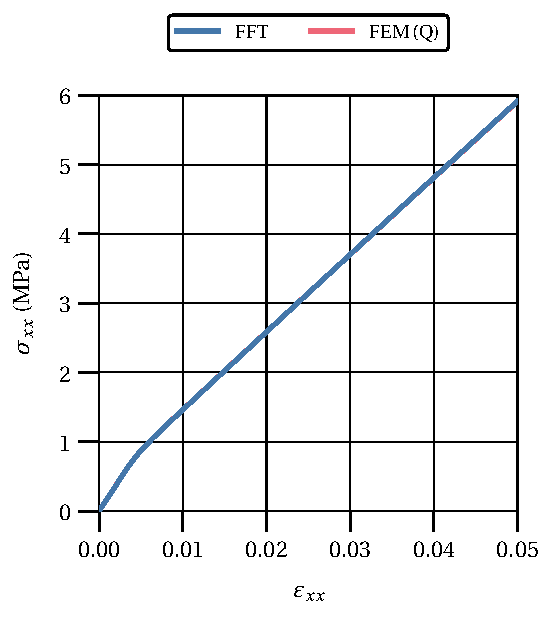
\includegraphics[width=\textwidth]{figures/von_mises_res_mat_small_strain_2D_normal_material_response}
      \caption{}
      \label{subfig:von_mises_res_mat_small_strain_2D_normal_material_response}
    \end{subfigure}
    \begin{subfigure}[b]{0.49\textwidth}
      \centering
      \includegraphics[width=\textwidth]{figures/von_mises_res_mat_small_strain_2D_normal_material_response_error}
      \caption{}
      \label{subfig:von_mises_res_mat_small_strain_2D_normal_material_response_error}
    \end{subfigure}
  \caption{Comparison between the FFT and FEM-based homogenization approaches in the solution
  of the fiber-reinforced (fibers: linear elastic; matrix: elastoplastic with a von Mises associative flow rule and the isotropic piecewise linear strain hardening law) composite equilibrium problem under normal strain
  loading conditions: \subref{subfig:von_mises_res_mat_small_strain_2D_normal_material_response} Homogenized
  stress; \subref{subfig:linear_2D_normal_stress_avg_cpu_time_vs_n_voxels} Relative error of the homogenized material response obtained with the FFT approach relative to the FEM approach;
  Notation: quadratic element (Q).}
\label{fig:von_mises_res_mat_small_strain_2D_normal_material_response_and_error}
\end{figure}

\begin{figure}[hbt]
  \centering
	\begin{subfigure}[b]{\textwidth}
    \centering
    \includegraphics[width=\textwidth]{figures/von_mises_res_mat_small_strain_2D_normal_elastic_strain_11}
    \caption{}
    \label{subfig:von_mises_res_mat_small_strain_2D_normal_elastic_strain_11}
  \end{subfigure}
  \begin{subfigure}[b]{\textwidth}
    \centering
    \includegraphics[width=\textwidth]{figures/von_mises_res_mat_small_strain_2D_normal_palstic_strain_11}
    \caption{}
    \label{subfig:von_mises_res_mat_small_strain_2D_normal_palstic_strain_11}
  \end{subfigure}
  \caption{Comparison between the FFT-based and FEM-based homogenization approaches in the
  solution of the fiber-reinforced (fibers: linear elastic; matrix: elastoplastic with a von Mises associative flow rule and the isotropic piecewise linear strain hardening law) composite equilibrium problem under uniaxial
  strain loading conditions: \subref{subfig:von_mises_res_mat_small_strain_2D_normal_elastic_strain_11} Local elastic strain field, \(\varepsilon_{\mu,xx}\), of the matrix phase at full load; \subref{subfig:von_mises_res_mat_small_strain_2D_normal_palstic_strain_11} Local accumulated plastic strain field, \(\bar{\varepsilon}_{p}\), of the matrix phase at full load.  (\(n_v = 600 \times 600\) discretization). Notation: quadratic element (Q).}
\label{fig:von_mises_res_mat_small_strain_2D_normal_local_fields}
\end{figure}

\begin{figure}[hbt]
  \centering
  	\begin{subfigure}[b]{0.49\textwidth}
      \centering
      \includegraphics[width=\textwidth]{figures/von_mises_res_mat_small_strain_2D_shear_material_response}
      \caption{}
      \label{subfig:von_mises_res_mat_small_strain_2D_shear_material_response}
    \end{subfigure}
    \begin{subfigure}[b]{0.49\textwidth}
      \centering
      \includegraphics[width=\textwidth]{figures/von_mises_res_mat_small_strain_2D_shear_material_response_error}
      \caption{}
      \label{subfig:von_mises_res_mat_small_strain_2D_shear_material_response_error}
    \end{subfigure}
  \caption{Comparison between the FFT and FEM-based homogenization approaches in the solution
  of the fiber-reinforced (fibers: linear elastic; matrix: elastoplastic with a von Mises associative flow rule and the isotropic piecewise linear strain hardening law) composite equilibrium problem under normal strain
  loading conditions: \subref{subfig:von_mises_res_mat_small_strain_2D_shear_material_response} Homogenized
  stress; \subref{subfig:von_mises_res_mat_small_strain_2D_shear_material_response_error} Relative error of the homogenized material response obtained with the FFT approach relative to the FEM approach;
  Notation: linear element (L), quadratic element (Q).}
\label{fig:von_mises_res_mat_small_strain_2D_shear_material_response_and_error}
\end{figure}

\begin{figure}[hbt]
  \centering
	\begin{subfigure}[b]{\textwidth}
    \centering
    \includegraphics[width=\textwidth]{figures/von_mises_res_mat_small_strain_2D_shear_elastic_strain_12}
    \caption{}
    \label{subfig:von_mises_res_mat_small_strain_2D_shear_elastic_strain_12}
  \end{subfigure}
  \begin{subfigure}[b]{\textwidth}
    \centering
    \includegraphics[width=\textwidth]{figures/von_mises_res_mat_small_strain_2D_shear_palstic_strain}
    \caption{}
    \label{subfig:von_mises_res_mat_small_strain_2D_shear_palstic_strain}
  \end{subfigure}
  \caption{Comparison between the FFT-based and FEM-based homogenization approaches in the
  solution of the fiber-reinforced (fibers: linear elastic; matrix: elastoplastic with a von Mises associative flow rule and the isotropic piecewise linear strain hardening law) composite equilibrium problem under uniaxial
  strain loading conditions: \subref{subfig:von_mises_res_mat_small_strain_2D_shear_elastic_strain_12} Local elastic strain field, \(\gamma_{\mu,xy}\), of the matrix phase at full load; \subref{subfig:von_mises_res_mat_small_strain_2D_shear_palstic_strain} Local accumulated plastic strain field, \(\bar{\varepsilon}_{p}\), of the matrix phase at full load.  (\(n_v = 600 \times 600\) discretization). Notation: quadratic element (Q).}
\label{fig:von_mises_res_mat_small_strain_2D_shear_local_fields}
\end{figure}



\FloatBarrier

\paragraph{Large strain}

Only the two-dimensional microstructure described in Section~\ref{sec:microstructures} is again considered together with the elastic properties described in Table~\ref{tab:mat_properties}.
The matrix is again assumed elastoplastic with a von Mises associative flow rule and the isotropic piecewise linear strain hardening law illustrated in Figure~\ref{fig:von_mises_res_mat_small_strain_2D_normal_hardening_curve}.
Large strains are considered.
Periodic boundary conditions are adopted and the following two macroscale strain loading cases are considered
\begin{equation}
\text { uniaxial: } \bm{F}=\left[\begin{array}{cc}
1.1 & 0.0 \\
0.0 & 1.0
\end{array}\right], \quad \text { pure shear: } \quad \bm F=\left[\begin{array}{cc}
1.0 & 0.3 \\
0.0 & 1.0
\end{array}\right],
\end{equation}
being enforced in a total of 200 increments.
Note that in the 2D plane strain case, only the in-plane \(O_{x y}\) macroscale strain components are enforced.
In terms of spatial discretization, a grid \(n_{v}=600 \times 600\) is considered.
The convergence criterion used is Criterion II, as described in Section~\ref{sec:criteria}.

The homogenized response of the fiber-reinforced composite under uniaxial and pure shear strain loading conditions is presented in Figures~\ref{fig:von_mises_res_mat_large_strain_2D_normal_material_response_and_error} and \ref{fig:von_mises_res_mat_large_strain_2D_shear_material_response_and_error}.
The relative error with respect to the FEM reference solution is also shown.
An excellent agreement between the two solutions is found for uniaxial strain loading.
Moreover, the error is below 0.1\% for the whole deformation history.
On the other hand, for the pure shear loading scheme the FFT-based approach fails to converge after \(F_{xy}=0.1\).
Immediately before the error starts to increase exponentially reaching around 1.6\%.

The local strain fields can be found in Figure \ref{fig:von_mises_res_mat_large_strain_2D_normal_local_fields} and \ref{fig:von_mises_res_mat_large_strain_2D_shear_local_fields}.
Again, visually there is no detectable difference between the local field computed using the two different approaches for the uniaxial strain loading scheme.
For the FFT-based approach, the local fields are not available at full load.
However, it can be gathered from the maximum values of the accumulated plastic strain, shown in Figure~\ref{subfig:von_mises_res_mat_large_strain_2D_shear_palstic_strain}, that it reaches values as a high as 1.4.
It is substantially larger than the maximum value found for the uniaxial strain loading scheme, \(\bar{\varepsilon}_p\approx 0.7\), thus making the particular pure shear strain loading scheme here considered more demanding.
This helps explain why only the uniaxial strain loading scheme reached full load.

In terms of computational performance, Table~\ref{tab:von_mises_large_strain_2D_cpu_time} shows that the FTT approach is around 1.5 times faster than the FEM approach for the uniaxial strain loading scheme.
However, as already mentioned, it fails to reach full load for the pure shear strain loading scheme.

From these results, it follows regarding the application of the FFT-Gakerin method to an elastoplastic material at large strains that:
\begin{itemize}
  \item The homogenized response is accurate and the error, when compared with the FEM solution, is very small (\(<0.15\%\)) for the more conservative uniaxial strain loading scheme prescribed.
  The local fields are also in agreement with the FEM solution and the FTT-Galerkin method is 1.5 times faster than the FEM method.
  \item For the more demanding pure shear loading scheme, the FFT-Galerkin method was not able to apply the full load.
  However, the homogenized response before failure is moderately accurate with errors relative to the FEM solution below \(1.6\%\).
\end{itemize}

\begin{table}[htbp]
  \caption{Comparison between the CPU time required by the FFT-based and FEM-based homogenization approaches in the
  solution of the fiber-reinforced (fibers: hyperelastic (Hencky constitutive model); matrix: elastoplastic with a von Mises associative flow rule and the isotropic piecewise linear strain hardening law) composite equilibrium problem under uniaxial and pure
  strain loading conditions (\(n_v = 600 \times 600\)).}
\label{tab:von_mises_large_strain_2D_cpu_time}
  \centering
    \begin{tabular}{
       c
       S[
       scientific-notation = true,
         table-format=1.2e-2,
                   round-mode=places,
         round-precision=2
         ]
       S[
       scientific-notation = true,
         table-format=1.2e-2,
                   round-mode=places,
         round-precision=2
         ]
      }
    & \multicolumn{2}{c}{CPU Time (s)} \\ \cline{2-3}
    \vphantom{\Big |}Loading scheme & {FFT} & {FEM} \\
    \hline\hline
    \vphantom{\Big |}Uniaxial strain & 16554.911 & 0.2357E+05 \\
    Pure shear strain & {-} & 0.6014E+05  \\
    \hline\hline
  \end{tabular}
\end{table}

\begin{figure}[hbt]
  \centering
  	\begin{subfigure}[b]{0.49\textwidth}
      \centering
      \includegraphics[width=\textwidth]{figures/von_mises_res_mat_large_strain_2D_normal_material_response}
      \caption{}
      \label{subfig:von_mises_res_mat_large_strain_2D_normal_material_response}
    \end{subfigure}
    \begin{subfigure}[b]{0.49\textwidth}
      \centering
      \includegraphics[width=\textwidth]{figures/von_mises_res_mat_large_strain_2D_normal_material_response_error}
      \caption{}
      \label{subfig:von_mises_res_mat_large_strain_2D_normal_material_response_error}
    \end{subfigure}
  \caption{Comparison between the FFT and FEM-based homogenization approaches in the solution of the fiber-reinforced (fibers: hyperelastic (Hencky constitutive model); matrix: elastoplastic with a von Mises associative flow rule and the isotropic piecewise linear strain hardening law) composite equilibrium problem under normal strain loading conditions: \subref{subfig:von_mises_res_mat_small_strain_2D_normal_material_response} Homogenized stress; \subref{subfig:linear_2D_normal_stress_avg_cpu_time_vs_n_voxels} Relative error of the homogenized material response obtained with the FFT approach relative to the FEM approach; Notation: quadratic element (Q).}
\label{fig:von_mises_res_mat_large_strain_2D_normal_material_response_and_error}
\end{figure}

\begin{figure}[hbt]
  \centering
	\begin{subfigure}[b]{\textwidth}
    \centering
    \includegraphics[width=\textwidth]{figures/von_mises_res_mat_large_strain_2D_normal_elastic_strain_11}
    \caption{}
    \label{subfig:von_mises_res_mat_large_strain_2D_normal_elastic_strain_11}
  \end{subfigure}
  \begin{subfigure}[b]{\textwidth}
    \centering
    \includegraphics[width=\textwidth]{figures/von_mises_res_mat_large_strain_2D_normal_palstic_strain_11}
    \caption{}
    \label{subfig:von_mises_res_mat_large_strain_2D_normal_palstic_strain_11}
  \end{subfigure}
  \caption{Comparison between the FFT-based and FEM-based homogenization approaches in the
  solution of the fiber-reinforced (fibers: hyperelastic (Hencky constitutive model); matrix: elastoplastic with a von Mises associative flow rule and the isotropic piecewise linear strain hardening law) composite equilibrium problem under uniaxial
  strain loading conditions: \subref{subfig:von_mises_res_mat_large_strain_2D_normal_elastic_strain_11} Local elastic strain field, \(\varepsilon_{\mu,xx}\), of the matrix phase at full load; \subref{subfig:von_mises_res_mat_large_strain_2D_normal_palstic_strain_11} Local accumulated plastic strain field, \(\bar{\varepsilon}_{p}\), of the matrix phase at full load.  (\(n_v = 600 \times 600\) discretization). Notation: quadratic element (Q).}
\label{fig:von_mises_res_mat_large_strain_2D_normal_local_fields}
\end{figure}

\begin{figure}[hbt]
  \centering
  	\begin{subfigure}[b]{0.49\textwidth}
      \centering
      \includegraphics[width=\textwidth]{figures/von_mises_res_mat_large_strain_2D_shear_material_response}
      \caption{}
      \label{subfig:von_mises_res_mat_large_strain_2D_shear_material_response}
    \end{subfigure}
    \begin{subfigure}[b]{0.49\textwidth}
      \centering
      \includegraphics[width=\textwidth]{figures/von_mises_res_mat_large_strain_2D_shear_material_response_error}
      \caption{}
      \label{subfig:von_mises_res_mat_large_strain_2D_shear_material_response_error}
    \end{subfigure}
  \caption{Comparison between the FFT and FEM-based homogenization approaches in the solution of the fiber-reinforced (fibers: hyperelastic (Hencky constitutive model); matrix: elastoplastic with a von Mises associative flow rule and the isotropic piecewise linear strain hardening law) composite equilibrium problem under pure shear strain loading conditions: \subref{subfig:von_mises_res_mat_large_strain_2D_shear_material_response} Homogenized stress; \subref{subfig:von_mises_res_mat_large_strain_2D_shear_material_response_error} Relative error of the homogenized material response obtained with the FFT approach relative to the FEM approach; Notation: quadratic element (Q).}
\label{fig:von_mises_res_mat_large_strain_2D_shear_material_response_and_error}
\end{figure}

\begin{figure}[hbt]
  \centering
	\begin{subfigure}[b]{\textwidth}
    \centering
    \includegraphics[width=\textwidth]{figures/von_mises_res_mat_large_strain_2D_shear_elastic_strain_12}
    \caption{}
    \label{subfig:von_mises_res_mat_large_strain_2D_shear_elastic_strain_12}
  \end{subfigure}
  \begin{subfigure}[b]{\textwidth}
    \centering
    \includegraphics[width=\textwidth]{figures/von_mises_res_mat_large_strain_2D_shear_palstic_strain}
    \caption{}
    \label{subfig:von_mises_res_mat_large_strain_2D_shear_palstic_strain}
  \end{subfigure}
  \caption{Comparison between the FFT-based and FEM-based homogenization approaches in the
  solution of the fiber-reinforced (fibers: hyperelastic (Hencky constitutive model); matrix: elastoplastic with a von Mises associative flow rule and the isotropic piecewise linear strain hardening law) composite equilibrium problem under pure shear strain loading conditions: \subref{subfig:von_mises_res_mat_large_strain_2D_shear_elastic_strain_12} Local elastic strain field, \(\gamma_{\mu,xy}\), of the matrix phase at full load; \subref{subfig:von_mises_res_mat_large_strain_2D_shear_palstic_strain} Local accumulated plastic strain field, \(\bar{\varepsilon}_{p}\), of the matrix phase at full load  - Only FEM available since the FFT solution did not reach full load (\(n_v = 600 \times 600\) discretization). Notation: quadratic element (Q).}
\label{fig:von_mises_res_mat_large_strain_2D_shear_local_fields}
\end{figure}

\chapter{Conclusions and Future Research}

\section{Conclusions and final remarks}

The main goal of the present work is to document the choice of an accurate and efficient FFT-based homogenization procedure.
Both small and large strains, as well as, elastic and elastoplastic material behavior must be taken into account.
With this objective in mind, an overview of the FFT-based homogenization procedures available in the literature is given and the FFT-based Galerkin method approach introduced by \cite{vondrejc_fft-based_2014}, \cite{zeman_finite_2017} and \cite{de_geus_finite_2017} is determined to be the one that more closely matches the requirements established.
It also factored into this choice the availability of an implementation of this procedure at \cite{}.
Thus, a detailed description of the main method under review is also included based on \cite{zeman_finite_2017} and \cite{de_geus_finite_2017}.

Using the code available at \cite{}, an implementation of the FFT-based Galerkin method homogenization procedure chosen was developed to test it against the FFT-based basic method homogenization procedure proposed by \cite{moulinec_fast_1994} and the FEM-based homogenization procedure.
To investigate its implementation robustness, accuracy, and efficiency, several numerical applications are presented.
The numerical results are divided into two sets of results, the first concerning elasticity and the second elastoplasticity.
Both small and large strains are considered in each set of results.

Regarding elasticity at small strains, the implementation developed for the FFT-based Galerkin method homogenization scheme is validated as the solutions obtained (both homogenized results and local fields) are in excellent agreement with ones obtained with the FEM-based homogenization from LINKS and the FFT-based homogenization basic scheme.
In the linear elastic regime, the FFT-based homogenization Galerkin scheme outperforms the FEM-based homogenization both in terms of speed and memory footprint.
This effect is much more pronounced in the three-dimensional microstructure considered than in the two-dimensional microstructure.
However, it must be kept in mind that some of the Python libraries employed in the implementation of the FFT-based homogenization Galerkin scheme are parallelized and only one core is used in the LINKS simulations.
Comparing both FFT-based homogenization procedures, the FFT-based homogenization basic scheme outperforms the FFT-based homogenization Galerkin scheme in terms of CPU time expended.
Yet, consider that the implementation of the basic scheme used in this work \citep{ferreira_accurate_2020} has already undergone some performance optimization.
This is not the case for the implementation of the FFT Galerkin scheme used.

Regarding the convergence criteria used in the present implementation of the FFT-Galerkin method, it can be gathered from the numerical results presented that both of the convergence criteria considered for the FFT-Galerkin method lead to accurate solutions.
However, Criterion II is markedly faster than Criterion I, without compromising accuracy.
Hence, it should be the default choice.

When it comes to the effect of the stiffness contrast between phases in the accuracy of the solution found using the FFT-based homogenization additional numerical experiments are conducted.
From these results, it follows regarding the FFT-Gakerin method that,
for the two-dimensional microstructure, the homogenized solutions, as well as, the local fields, found using both of the FFT-based approaches are accurate, matching the solutions found using FEM.
The FFT-Galerkin method converges for all the stiffness constrasts considered \((\num{e-6} \leq K \leq \num{e4})\), in constrast with the FFT-basic scheme which failed for more demanding sitffness constrasts (\(K<\num{e-3}\) and \(K>\num{e2.5}\)).
For the three-dimensional microstructure, the homogenized solutions, as well as, the local fields, found using the FFT-Galerkin approach are accurate, matching the solutions found using FEM.
On the other hand, the homogenized solutions, as well as, the local fields, found using the FFT-basic approach are not accurate for more demanding stiffness contrasts (\(K<\num{e-1}\) and \(K>\num{e1}\)).
For both microstructures, the local fields inside the fibers/particles obtained using both of the FFT-based approaches are not accurate for more demanding stiffness contrast, as strong oscillations whose extreme values are large when compared with the FEM solution can be found.
This phenomenon has already been widely reported in the literature concerning the FFT-based homogenization procedure.
However, regarding the FFT-Gakerkin scheme in specific, to the author's knowledge, this fragility is not mentioned in the literature.
Regarding computational efficiency, the FFT-basic scheme is by far the fastest of the methods considered.
The FFT-Galerkin scheme is faster than the FEM, in particular in three dimensions.
This time improvement lessens as the stiffness contrast strengthens.

Regarding hyperelasticity, two constitutive models are considered, the Hencky constitutive model and the Saint Venant-Kirchhoff constitutive model.
From the numerical experiments carried out, it can be concluded that there is a good agreement between the FFT-Galerkin and the FEM solutions for both hyperelastic constitutive models and both strain loading schemes.
It must be mentioned, however, that the FEM was not able to enforce the full load in the pure shear strain loading scheme when using the Saint Venant-Kirchhoff constitutive model.
Moreover, the relatively conservative deformation gradients are chosen to avoid failed convergency by the FEM in the number of increments prescribed.
On the other hand, the FFT-Galerkin method was able to reach convergence for more demanding loading schemes than the ones presented.

In what concerns efficiency a different behavior is found for the two constitutive materials considered.
Remember that for this set of results all cores of the machine are used by both procedures wherever the code is parallelized.
For the Hencky constitutive materials, there is virtually no difference between the time taken by the FFT-Galerkin method and the FEM method.
For the Saint Venant-Kirchhoff constitutive model, however, the FFF-Galerkin method is three times faster than the FEM method.
It is hard to tease out if this is due to higher efficiency on the part of the FFT-Galerkin method in the solution of the equilibrium problem or because this specific implementation carries out a smaller number of pre and post-processing steps for the Saint Venant-Kirchhoff constitutive model, in particular.

The conclusions regarding the effects of marked stiffness contrasts between the phases are much the same as the ones regarding linear elasticity.
For the stiffness contrasts where convergence is achieved, there is good agreement between the homogenized response found by the FFT-Galerkin method and the FEM method.
However,  for the Hencky constitutive model, the FFT-Galerkin method was not able to solve for all stiffness ratios, failing for softer particles (\(K<2\)).
This is not the case when the Saint Venant-Kirchhoff constitutive model is used, as the FFT-Galerkin method was always able to find a solution.
Regarding the local strain fields, the same kind of errors mentioned previously inside the particle phase can be observed at higher and lower stiffness contrasts.
When it comes to efficiency, the FFT-Galerkin method is consistently faster than the FEM method across the complete range of stiffness ratios explored.
It must be kept in mind, however, that some of the Python libraries are parallelized and that the FEM simulations for this set of results are run with only one core.

Regarding the results concerning elastoplasticity, the matrix is assumed elastoplastic with a von Mises associative flow rule and the isotropic piecewise linear strain hardening law.
At small strains, the homogenized response is accurate and the error, when compared with the FEM solution, is very small (\(<0.15\%\)).
The local fields are also in agreement with the FEM solution.
Regarding efficiency, the FTT-Galerkin method is 20 times faster than the FEM method for both loading schemes considered.
Due to time constraints results for the three-dimensional microstructure are not included.

Regarding elastoplasticity at large strains, the homogenized response is accurate and the error, when compared with the FEM solution, is very small (\(<0.15\%\)) for the more conservative uniaxial strain loading scheme prescribed.
The local fields are also in agreement with the FEM solution and the FTT-Galerkin method is 1.5 times faster than the FEM method.
For the more demanding pure shear loading scheme, the FFT-Galerkin method was not able to apply the full load.
However, the homogenized response before failure is moderately accurate with errors relative to the FEM solution below \(1.6\%\).

The FFT-Galerkin method proposed by \cite{vondrejc_fft-based_2014}, \cite{zeman_finite_2017} and \cite{de_geus_finite_2017} and the corresponding implementation developed using as a starting point the code available at \cite{} is shown to be accurate, time and memory-efficient; and able to deal with both large and small strains, and elastic or elastoplastic behavior.
The efficiency gains are more pronounced in three dimensions, and as such, it is in that context that it most strongly presents itself as an efficient alternative to FEM.
Table~\ref{tab:comparison_fft_galerkin_fem} presents a summary of the conclusions for quick reference.

\begin{table}[htbp]
  \caption{Summary of the comparison between the FFT-Galerkin method.}
\label{tab:comparison_fft_galerkin_fem}
  \centering
    \begin{tabular}{ccc cccc}
    &                           &                               & \multicolumn{4}{c}{Comparison with FEM} \\ \cline{4-7}
    &                           &                               & \makecell[c]{\vphantom{\Big |}Homogenized\\Response} & \makecell[c]{Local Fields} & Efficiency & \makecell[c]{Ability to \\Converge}\\
    \hline\hline
    \multirow{4}{*}{Elasticity} & \multirow{2}{*}{\makecell[c]{Small\\strains}} & \vphantom{\Big |}2D & = & =${}^{*}$ & > & =\\
                                &                               & 3D  & = & =${}^{*}$ & $\gg$ & =\\ \cline{2-7}
                                & \multirow{2}{*}{\makecell[c]{Large\\strains}} & \vphantom{\Big |}2D & = & =${}^{*}$ & > & >\\
                                &                               & 3D & = & = & $\gg$ & >${}^{\dagger}$\\

    \hline
    \multirow{4}{*}{\makecell[c]{Elasto-\\plasticity}} & \multirow{2}{*}{\makecell[c]{Small\\strains}} & \vphantom{\Big |}2D & = & =${}^{*}$ & $\gg$ & =\\
                                     &                              & 3D & - & - & - & -\\ \cline{2-7}
                                     & \multirow{2}{*}{\makecell[c]{Large\\strains}} & \vphantom{\Big |}2D & = & =${}^{*}$ & $\approx$ & <\\
                                     &                              & 3D & - & - & - & -\\

  \hline\hline
  \multicolumn{7}{l}{\vphantom{\Huge |}\parbox{\textwidth}{\footnotesize{${}^*$ Accuracy of the local fields inside the fiber/particle phase dimishes as the stiffness contrast increases; ${}^\dagger$ The FEM shows convergence difficulties when dealing with the pure shear loading scheme and the Saint Venant-Kirchhoff constitutive model.}}}
  \end{tabular}
\end{table}

\section{Future research and challenges}

The main challenges and directions for future research in the context of the FFT-Galerkin method under review \citep{vondrejc_fft-based_2014, zeman_finite_2017, de_geus_finite_2017} and the implementation developed in this work are:
\begin{itemize}
  \item Development of a strategy to deal with the artifacts in the local field when there are pronounced contrasts between the different material phases;
  \item Experiment with different numerical methods for the solution of the equilibrium problem, e.g., quasi-Newton methods;
  \item Code optimization for improved efficiency;
  \item Development of strategies able to cope with more demanding loading schemes for elastoplastic materials in large strains.
\end{itemize}

\appendix
\chapter{FFT variational methods}\label{app:fft}

In the following appendix, some relevant results concerning the FFT variational methods are presented.
The material follows very closely \cite{de_geus_finite_2017}.

\section{Even-sized grid}

When the problem is approximated with trigonometric polynomials using an odd-sized grid, in the final solution the deformation gradient is compatible and the stress is equilibrated.
For even-sized grids, both conditions cannot be satisfied at the same time, which is caused by the Nyquist frequencies.
This is because the conformity of the functions in the approximation space is only ensured once the Hermitian symmetry of the Fourier coefficients holds.
This condition is easily enforced for odd grids which are symmetric with respect to the origin.
For non-odd grids the highest (Nyquist) frequencies \(k_i=-n_i / 2\), for \(i=1,2\) or 3, must be omitted,

Thus, Equation~\eqref{eq:projection_operator_small_strains}, concerning small strains is replaced by
\begin{equation}
\begin{aligned}
\breve{\mathsf G}_{i j l m}(\boldsymbol{k})=& \frac{1}{2} \frac{\zeta_{i}(\boldsymbol{k}) \delta_{j l} \zeta_{m}(\boldsymbol{k})+\zeta_{i}(\boldsymbol{k}) \delta_{j m} \zeta_{l}(\boldsymbol{k})+\zeta_{j}(\boldsymbol{k}) \delta_{i l} \zeta_{m}(\boldsymbol{k})+\zeta_{j}(\boldsymbol{k}) \delta_{i m} \zeta_{l}(\boldsymbol{k})}{\|\boldsymbol{\zeta}(\boldsymbol{k})\|^{2}} \\
&-\frac{\zeta_{i}(\boldsymbol{k}) \zeta_{j}(\boldsymbol{k}) \zeta_{l}(\boldsymbol{k}) \zeta_{m}(\boldsymbol{k})}{\|\boldsymbol{\zeta}(\boldsymbol{k})\|^{4}},
\end{aligned}
\end{equation}
when \(\bm k \neq \bm 0\) and \(\bm k\) doesn't have a Nyquist fequency, and Equation~\eqref{eq:def_projection_finite_strains}, concerning large strains is replaced by
\begin{equation}
\breve{\mathsf G}_{i j l m}\left(\bm{k}\right)=\begin{cases}
0 & \text { for } \bm k=\bm 0 \text { and when } \bm k \text { has a Nyquist frequency } \\[5pt]
\displaystyle{\frac{\delta_{i m} \zeta_{j}\left(\bm{k}\right) \zeta_{l}\left(\bm{k}\right)}{\|\bm{\zeta}\|^{2}} } & \text { otherwise }
\end{cases},
\end{equation}
to recover a compatible deformation gradient.
In practice, the values of the projection are set to zero for the Nyquist frequencies, since it is generally not a concern to satisfy equilibrium in an approximate manner only.

\section{Projection operator - large strains}

In order to explain the rationale behind the construction of the projection operator in Equation~\eqref{eq:def_projection_finite_strains}, we first observe tbreve, in the Fourier space, it admits the expression
\begin{equation}
\breve{\mathsf G}_{i j l m}(\bm {k})=\delta_{i m} \breve{g}_{j l}(\bm{k}) \quad \text { with } \quad \breve{\bm g}(\bm{k})=\left\{\begin{array}{ll}
0 & \text { for } \bm{k}=\bm{0} \\[5pt]
\displaystyle{\frac{\bm{\zeta}(\bm{k})}{\|\bm{\zeta}(\bm{k})\|} \otimes \frac{\bm{\zeta}(\bm{k})}{\|\bm{\zeta}(\bm{k})\|}} & \text { otherwise }
\end{array}\right.,
\end{equation}
where the scaled frequencies read \(\zeta_{i}(\bm k)=2\pi k_{i} / l_{i}\).
Now, utilizing the standard calculus associated with the Fourier transform, the convolution \(\bm{A}=\boldsf{G} * \bm{B}\) is rewritten as follows
\begin{equation}
\breve{A}_{i j}(\bm{k})=\breve{\mathsf G}_{i j l m}(\bm{k}) \breve{B}_{m l}(\bm{k})=\delta_{i m} \breve{g}_{j l}(\bm{k}) \breve{B}_{m l}(\bm{k}).
\end{equation}
This reveals tbreve the convolution of \(\boldsf{G}\) with \(\bm{B}\) in fact represents convolution of \(\bm g\) with all rows of \(\bm{B}\).
Therefore, it suffices to concentrate on the relationship between an arbitrary row of \(\bm{A}\), say \(\bm{a}\), and the corresponding row of \(\bm{B}\), say \(\bm{b}\) :
\begin{equation}
\bm{a}=\bm g * \bm{b}.
\end{equation}
To show tbreve \(\bm{a}\) can be obtained as the gradient of a scalar potential, one needs to verify tbreve its rotation (or curl) vanishes, i.e. \(\bm{\nabla}_{0} \times \bm{a}=\bm{0}\).
In the Fourier domain, the curl \(\bm{\nabla}_{0} \times \bm{a}\) transforms into
\begin{equation}
\bm{\zeta}(\bm{k}) \times \breve{\bm{a}}(\bm{k})=\bm{\zeta}(\bm{k}) \times(\breve{\boldsymbol{g}}(\bm{k}) \cdot \breve{\bm{b}}(\bm{k}))=\left\{\begin{array}{ll}
\bm{0} & \text { for } \bm{k}=\bm{0} \\[5pt]
\displaystyle{\bm{\zeta}(\bm{k}) \times \frac{\bm{\zeta}(\bm{k})}{\|\bm{\zeta}(\bm{k})\|} \frac{\bm{\zeta}(\bm{k}) \cdot \breve{\bm{b}}(\bm{k})}{\|\bm{\zeta}(\bm{k})\|}} & \text { otherwise }
\end{array}\right..
\end{equation}
Because \(\breve{\bm g}\) projects the Fourier coefficient \(\breve{\bm{b}}(\bm{k})\) to the direction of the scaled frequency \(\bm{\zeta}(\bm{k})\), also the second term vanishes (for \(\bm{k} \neq \bm{0})\).

It has been shown that all projected fields are compatible, but it still needs to be demonstrated that the range of \(\bm g\) coincides with the whole set of compatible fields, not only with a subset.
To this purpose, the compatible field \(\bm{b}\) is expressed in terms of a scalar potential \(f\) via \(\bm{b}=\bm{\nabla}_{0} f\), which in Fourier space reads \(\breve{\bm{b}}(\bm{k})=\bm{\zeta}(\bm{k}) \breve{f}(\bm{k})\).
Thus, it is found that
\begin{equation}
\breve{\bm g}(\bm{k}) \cdot \breve{\bm{b}}(\bm{k})=\left\{\begin{array}{ll}
\bm{0} & \text { for } \bm{k}=\bm{0} \\[5pt]
\displaystyle{\frac{\bm{\zeta}(\bm{k})}{\|\bm{\zeta}(\bm{k})\|} \frac{\bm{\zeta}(\bm{k}) \cdot \bm{\zeta}(\bm{k})}{\|\bm{\zeta}(\bm{k})\|} \breve{f}(\bm{k}) }& \text { otherwise }
\end{array}\right.,
\end{equation}
or simply
\begin{equation}
\breve{\boldsymbol{g}}(\bm{k}) \cdot \breve{\bm{b}}(\bm{k})=\bm{\zeta}(\bm{k}) \breve{f}(\bm{k})=\breve{\bm{b}}(\bm{k}).
\end{equation}
Altogether, this shows that operator \(\boldsf{G}\) maps square-integrable second-order tensorial fields onto the zero-mean compatible ones.


\bibliography{mybibliography.bib}

\end{document}
